
\section[{Representation of Primary Sources}]{Representation of Primary Sources}\label{PH}\par
This chapter describes elements that may be used to represent primary source materials, such as manuscripts, printed books, ephemera, or other textual documents. Some of these specialized elements, particularly at phrase-level, add to the other elements available within \hyperref[TEI.text]{<text>} to deal with textual phenomena more specific to primary source transcription. Other structural and block-level elements described here can be used to represent primary source materials by prioritizing the encoding of their spatial features over their logical textual structure (that is, the elements described in chapter \textit{\hyperref[DS]{4.\ Default Text Structure}}). These elements, \hyperref[TEI.facsimile]{<facsimile>}, \hyperref[TEI.sourceDoc]{<sourceDoc>}, and their children, may be used in parallel and in combination with an encoding of logical text structures with \hyperref[TEI.text]{<text>}, or as standalone representations. The element \hyperref[TEI.sourceDoc]{<sourceDoc>} in particular provides a way of combining facsimile and transcriptions by embedding transcribed text. This approach focuses on physical and textual features that can be primarily described spatially, such as the sequence of pages in a manuscript, or the layout of a printed page. This is not meant to be the only way of transcribing primary sources in TEI, or even a preferred way; which approach is more appropriate will depend on the specific needs of your project.\par
Although this chapter discusses manuscript materials more frequently than other forms of written text, most of the recommendations presented are equally applicable to facsimiles of a wide variety of media, including printed matter, monumental inscriptions, and art. Each medium has its own vocabulary of agents. In the following examples, terms such as ‘scribe’, ‘author’, ‘editor’, ‘annotator’ or ‘corrector’ may be re-interpreted in terms more appropriate to the medium being transcribed. In printed material, for example, the ‘compositor’ plays a role analogous to the ‘scribe’, while in an authorial manuscript, the ‘author’ and the ‘scribe’ are the same person.\par
This module may be used in conjunction with other modules. These recommendations are not intended to meet every transcriptional circumstance likely to be faced by any scholar. They are intended rather as a base to enable encoding of the most common phenomena found in the course of scholarly transcription of primary source materials. These guidelines do not address the encoding of physical description of textual witnesses: the materials of the carrier, the medium of the inscribing implement, the organisation of the carrier materials themselves (such as quiring, collation), authorial instructions or scribal markup, etc., except insofar as these are involved in the broader question of manuscript description, as addressed by the \textsf{msdescription} module described in chapter \textit{\hyperref[MS]{10.\ Manuscript Description}}.\par
This chapter begins by describing elements for handling digitally-encoded images of primary source materials for the purpose of creating digital facsimiles using the \hyperref[TEI.facsimile]{<facsimile>} element (\textit{\hyperref[PHFAX]{11.1.\ Digital Facsimiles}}).\par
The next section (\textit{\hyperref[PH-transcr]{11.2.\ Combining Transcription with Facsimile}}) describes two ways of combining a facsimile images with a transcription; either by referencing a parallel transcription in \hyperref[TEI.text]{<text>}, or by providing an ‘embedded’ transcription that prioritizes the encoding of a resource’s spatial features via the \hyperref[TEI.sourceDoc]{<sourceDoc>} element and a number of transcriptional elements.\par
Section \textit{\hyperref[PHST]{11.3.\ Scope of Transcriptions}} documents elements that support scholars in recording information about specific features of the text written on its physical carrier, such as \textit{\hyperref[PHCH]{11.3.1.\ Altered, Corrected, and Erroneous Texts}} and \textit{\hyperref[PHPH]{11.3.2.\ Hands and Responsibility}}\par
Section \textit{\hyperref[PHLAY]{11.4.\ Aspects of Layout}} describes how complex page layouts may be represented.\par
Section \textit{\hyperref[PHSK]{11.6.\ Headers, Footers, and Similar Matter}} introduces the element \hyperref[TEI.fw]{<fw>} (\textit{forme work}) for encoding material repeated from page to page that falls outside the stream of the text.\par
Section \textit{\hyperref[PH-changes]{11.7.\ Identifying Changes and Revisions}} describes how to document changes made during the production or revision of a primary source.\par
The chapter concludes with a technical overview of the structure and organization of the module described here. Some elements from other chapters are recontexualized for situations involving the transcription of primary source materials, whether within \hyperref[TEI.text]{<text>} or \hyperref[TEI.sourceDoc]{<sourceDoc>}. Therefore, this overview should be read in conjunction with chapters \textit{\hyperref[CO]{3.\ Elements Available in All TEI Documents}} and \textit{\hyperref[WD]{5.\ Characters, Glyphs, and Writing Modes}}.
\subsection[{Digital Facsimiles}]{Digital Facsimiles}\label{PHFAX}\par
A common approach in the TEI to representing pre-existing sources involves transcribing or otherwise converting sources into character form before marking them up. However, it is also a common practice to make a different form of ‘digital text’ that is instead composed of digital images of the original source, typically one per page, or other written surface. We call such a resource a \textit{digital facsimile}. A digital facsimile may, in the simplest case, just consist of a collection of images, with some metadata to identify them and the source materials portrayed. It may sometimes contain a variety of images of the same source pages, perhaps of different resolutions, or of different kinds. Such a collection may form part of any kind of document, for example a commentary of a codicological or paleographic nature, where there is a need to align explanatory text with image data. It may also be complemented by a transcribed or encoded version of the original source, which may be linked to the page images or ‘embedded’ as discussed in \textit{\hyperref[PH-transcr]{11.2.\ Combining Transcription with Facsimile}}. In this section we present elements designed to support these various possibilities and discuss the associated mechanisms provided by these Guidelines.\par
When this module is included in a schema, the class \textsf{att.global} is extended to include two new pointer attributes, {\itshape facs} and {\itshape change}: 
\begin{sansreflist}
  
\item [\textbf{att.global.facs}] provides an attribute used to express correspondence between an element containing transcribed text and all or part of an image representing that text.\hfil\\[-10pt]\begin{sansreflist}
    \item[@{\itshape facs}]
  (facsimile) points to all or part of an image which corresponds with the content of the element.
\end{sansreflist}  
\item [\textbf{att.global.change}] supplies the {\itshape change} attribute, allowing its member elements to specify one or more states or revision campaigns with which they are associated.\hfil\\[-10pt]\begin{sansreflist}
    \item[@{\itshape change}]
  points to one or more \hyperref[TEI.change]{<change>} elements documenting a state or revision campaign to which the element bearing this attribute and its children have been assigned by the encoder.
\end{sansreflist}  
\end{sansreflist}
 The {\itshape change} attribute is discussed further below in section \textit{\hyperref[PH-changes]{11.7.\ Identifying Changes and Revisions}}. The {\itshape facs} attribute is used to associate any element in a transcription with an image of the corresponding part of the source, by means of the usual URI pointing mechanism. \par
In the simple case where a digital text is composed of page images, the {\itshape facs} attribute on the \hyperref[TEI.pb]{<pb>} element may be used to associate each image with an appropriate point in the text: \par\bgroup\index{TEI=<TEI>|exampleindex}\index{teiHeader=<teiHeader>|exampleindex}\index{text=<text>|exampleindex}\index{pb=<pb>|exampleindex}\index{facs=@facs!<pb>|exampleindex}\index{pb=<pb>|exampleindex}\index{facs=@facs!<pb>|exampleindex}\exampleFont \begin{shaded}\noindent\mbox{}{<\textbf{TEI} xmlns="http://www.tei-c.org/ns/1.0">}\mbox{}\newline 
\hspace*{1em}{<\textbf{teiHeader}>}\mbox{}\newline 
\textit{<!--...-->}\mbox{}\newline 
\hspace*{1em}{</\textbf{teiHeader}>}\mbox{}\newline 
\hspace*{1em}{<\textbf{text}>}\mbox{}\newline 
\hspace*{1em}\hspace*{1em}{<\textbf{pb}\hspace*{1em}{facs}="{page1.png}"/>}\mbox{}\newline 
\textit{<!-- text contained on page 1 is encoded here -->}\mbox{}\newline 
\hspace*{1em}\hspace*{1em}{<\textbf{pb}\hspace*{1em}{facs}="{page2.png}"/>}\mbox{}\newline 
\textit{<!-- text contained on page 2 is encoded here -->}\mbox{}\newline 
\hspace*{1em}{</\textbf{text}>}\mbox{}\newline 
{</\textbf{TEI}>}\end{shaded}\egroup\par \noindent  By convention, this encoding indicates that the image indicated by the {\itshape facs} attribute represents the whole of the text following the \hyperref[TEI.pb]{<pb>} (page beginning) element, up to the next \hyperref[TEI.pb]{<pb>} element. Any convenient milestone element (see further \textit{\hyperref[CORS5]{3.11.3.\ Milestone Elements}}) could be used in the same way; for example if the images represent individual columns, the \hyperref[TEI.cb]{<cb>} element might be used. Though simple, this method has some drawbacks. It does not scale well to more complex cases where, for example, the images do not correspond exactly with transcribed pages, or where the intention is to align specific marked up elements with detailed images, or parts of images. The management of information about the images may become more difficult if references to them are scattered through many files rather than being concentrated in a single identifiable location. Nevertheless, this solution may be adequate for many straightforward ‘digital library’ applications.\par
The recommended approach to encoding facsimiles is instead to use the {\itshape facs} attribute in conjunction with the elements \hyperref[TEI.facsimile]{<facsimile>} or \hyperref[TEI.sourceDoc]{<sourceDoc>}, and the elements \hyperref[TEI.surface]{<surface>}, \hyperref[TEI.surfaceGrp]{<surfaceGrp>}, and \hyperref[TEI.zone]{<zone>}, which are also provided by this module. These elements make it possible to accommodate multiple images of each page, as well as to record the position and relative size of elements identified on any kind of written surface and to link such elements with digital facsimile images of them. Typical applications include the provision of full text search in ‘digital facsimile editions’, and ways of annotating graphics, for example so as to identify individuals appearing in group portraits and link them to data about the people represented.\par
The following elements are available to represent components of a digital facsimile: 
\begin{sansreflist}
  
\item [\textbf{<facsimile>}] contains a representation of some written source in the form of a set of images rather than as transcribed or encoded text.
\item [\textbf{<sourceDoc>}] contains a transcription or other representation of a single source document potentially forming part of a \textit{dossier génétique} or collection of sources.
\item [\textbf{<surface>}] defines a written surface as a two-dimensional coordinate space, optionally grouping one or more graphic representations of that space, zones of interest within that space, and transcriptions of the writing within them.
\item [\textbf{<surfaceGrp>}] defines any kind of useful grouping of written surfaces, for example the recto and verso of a single leaf, which the encoder wishes to treat as a single unit.
\item [\textbf{<zone>}] defines any two-dimensional area within a \hyperref[TEI.surface]{<surface>} element.\hfil\\[-10pt]\begin{sansreflist}
    \item[@{\itshape points [att.coordinated]}]
  identifies a two dimensional area by means of a series of pairs of numbers, each of which gives the x,y coordinates of a point on a line enclosing the area.
\end{sansreflist}  
\item [\textbf{<path>}] (path) defines any line passing through two or more points within a \hyperref[TEI.surface]{<surface>} element.\hfil\\[-10pt]\begin{sansreflist}
    \item[@{\itshape points}]
  identifies a line within the container or bounding box specified by the parent element by means of a series of two or more pairs of numbers, each of which gives the x,y coordinates of a point on the line.
\end{sansreflist}  
\end{sansreflist}
\par
Either of the \hyperref[TEI.facsimile]{<facsimile>} or \hyperref[TEI.sourceDoc]{<sourceDoc>} elements may be used to represent a digital facsimile. Either may appear within a TEI document along with, or instead of, the \hyperref[TEI.text]{<text>} element introduced in section \textit{\hyperref[DS]{4.\ Default Text Structure}}. The \hyperref[TEI.sourceDoc]{<sourceDoc>} element is used when a digital facsimile contains a transcription that prioritizes the encoding of the spatial features and layout of a text document over the text’s logical textual structure; the \hyperref[TEI.text]{<text>} element should be used when it contains a textual transcription focused on its logical features. When the digital facsimile contains only images, however, only \hyperref[TEI.facsimile]{<facsimile>} elements should be used. In this section, we first discuss the simpler case, returning to the use of the \hyperref[TEI.sourceDoc]{<sourceDoc>} element in section \textit{\hyperref[PH-transcr]{11.2.\ Combining Transcription with Facsimile}} below. When this module is selected therefore, a legal TEI document may thus comprise any of the following: \begin{itemize}
\item a TEI header and a text element
\item a TEI header and a facsimile element
\item a TEI header and a sourceDoc element
\item a TEI header, a facsimile element, and a text element
\item a TEI header, one or more sourceDoc or facsimile elements, and a text element
\end{itemize} \par
Like the \hyperref[TEI.text]{<text>} element, a \hyperref[TEI.facsimile]{<facsimile>} element may also contain an optional \hyperref[TEI.front]{<front>} or \hyperref[TEI.back]{<back>} element, used in the same way as described in sections \textit{\hyperref[DSFRONT]{4.5.\ Front Matter}} and \textit{\hyperref[DSBACK]{4.7.\ Back Matter}}.\par
In the simplest case, a facsimile just contains a series of \hyperref[TEI.graphic]{<graphic>} elements, each of which identifies an image file: \par\bgroup\index{facsimile=<facsimile>|exampleindex}\index{graphic=<graphic>|exampleindex}\index{url=@url!<graphic>|exampleindex}\index{graphic=<graphic>|exampleindex}\index{url=@url!<graphic>|exampleindex}\index{graphic=<graphic>|exampleindex}\index{url=@url!<graphic>|exampleindex}\index{graphic=<graphic>|exampleindex}\index{url=@url!<graphic>|exampleindex}\exampleFont \begin{shaded}\noindent\mbox{}{<\textbf{facsimile}>}\mbox{}\newline 
\hspace*{1em}{<\textbf{graphic}\hspace*{1em}{url}="{page1.png}"/>}\mbox{}\newline 
\hspace*{1em}{<\textbf{graphic}\hspace*{1em}{url}="{page2.png}"/>}\mbox{}\newline 
\hspace*{1em}{<\textbf{graphic}\hspace*{1em}{url}="{page3.png}"/>}\mbox{}\newline 
\hspace*{1em}{<\textbf{graphic}\hspace*{1em}{url}="{page4.png}"/>}\mbox{}\newline 
{</\textbf{facsimile}>}\end{shaded}\egroup\par \noindent  If desired, the \hyperref[TEI.binaryObject]{<binaryObject>} element described in \textit{\hyperref[COGR]{3.10.\ Graphics and Other Non-textual Components}} (or any other element from the \textsf{model.graphicLike} class) can be used instead of a \hyperref[TEI.graphic]{<graphic>}.\par
In this simple case, the four page images are understood to represent the complete facsimile, and are to be read in the sequence given. Suppose, however, that the second page of this particular work is available both as an ordinary photograph and as an infra-red image, or in two different resolutions. The \hyperref[TEI.surface]{<surface>} element may be used to group the two image files, since these correspond with the same area of the work: \par\bgroup\index{facsimile=<facsimile>|exampleindex}\index{graphic=<graphic>|exampleindex}\index{url=@url!<graphic>|exampleindex}\index{surface=<surface>|exampleindex}\index{graphic=<graphic>|exampleindex}\index{url=@url!<graphic>|exampleindex}\index{graphic=<graphic>|exampleindex}\index{url=@url!<graphic>|exampleindex}\index{graphic=<graphic>|exampleindex}\index{url=@url!<graphic>|exampleindex}\index{graphic=<graphic>|exampleindex}\index{url=@url!<graphic>|exampleindex}\exampleFont \begin{shaded}\noindent\mbox{}{<\textbf{facsimile}>}\mbox{}\newline 
\hspace*{1em}{<\textbf{graphic}\hspace*{1em}{url}="{page1.png}"/>}\mbox{}\newline 
\hspace*{1em}{<\textbf{surface}>}\mbox{}\newline 
\hspace*{1em}\hspace*{1em}{<\textbf{graphic}\hspace*{1em}{url}="{page2-highRes.png}"/>}\mbox{}\newline 
\hspace*{1em}\hspace*{1em}{<\textbf{graphic}\hspace*{1em}{url}="{page2-lowRes.png}"/>}\mbox{}\newline 
\hspace*{1em}{</\textbf{surface}>}\mbox{}\newline 
\hspace*{1em}{<\textbf{graphic}\hspace*{1em}{url}="{page3.png}"/>}\mbox{}\newline 
\hspace*{1em}{<\textbf{graphic}\hspace*{1em}{url}="{page4.png}"/>}\mbox{}\newline 
{</\textbf{facsimile}>}\end{shaded}\egroup\par \par
The \hyperref[TEI.surface]{<surface>} element provides a way of indicating that the two images of page2 represent the same surface within the source material. A \textit{surface} might be one side of a piece of paper or parchment, an opening in a codex treated as a single surface by the writer, a face of a monument, a billboard, a membrane of a scroll, or indeed any two-dimensional surface, of any size.\par
The \hyperref[TEI.surfaceGrp]{<surfaceGrp>} element may be used to indicate that two (or more) surfaces are associated in some way, for example because they represent the recto and verso of the same leaf, as in this example: \par\bgroup\index{facsimile=<facsimile>|exampleindex}\index{surfaceGrp=<surfaceGrp>|exampleindex}\index{n=@n!<surfaceGrp>|exampleindex}\index{surface=<surface>|exampleindex}\index{graphic=<graphic>|exampleindex}\index{url=@url!<graphic>|exampleindex}\index{surface=<surface>|exampleindex}\index{graphic=<graphic>|exampleindex}\index{url=@url!<graphic>|exampleindex}\index{graphic=<graphic>|exampleindex}\index{url=@url!<graphic>|exampleindex}\exampleFont \begin{shaded}\noindent\mbox{}{<\textbf{facsimile}>}\mbox{}\newline 
\hspace*{1em}{<\textbf{surfaceGrp}\hspace*{1em}{n}="{leaf1}">}\mbox{}\newline 
\hspace*{1em}\hspace*{1em}{<\textbf{surface}>}\mbox{}\newline 
\hspace*{1em}\hspace*{1em}\hspace*{1em}{<\textbf{graphic}\hspace*{1em}{url}="{page1.png}"/>}\mbox{}\newline 
\hspace*{1em}\hspace*{1em}{</\textbf{surface}>}\mbox{}\newline 
\hspace*{1em}\hspace*{1em}{<\textbf{surface}>}\mbox{}\newline 
\hspace*{1em}\hspace*{1em}\hspace*{1em}{<\textbf{graphic}\hspace*{1em}{url}="{page2-highRes.png}"/>}\mbox{}\newline 
\hspace*{1em}\hspace*{1em}\hspace*{1em}{<\textbf{graphic}\hspace*{1em}{url}="{page2-lowRes.png}"/>}\mbox{}\newline 
\hspace*{1em}\hspace*{1em}{</\textbf{surface}>}\mbox{}\newline 
\hspace*{1em}{</\textbf{surfaceGrp}>}\mbox{}\newline 
{</\textbf{facsimile}>}\end{shaded}\egroup\par \noindent  The \hyperref[TEI.surfaceGrp]{<surfaceGrp>} element may also be useful as a means of identifying other groups of written surfaces, such as adjacent faces of a monument, or gatherings of leaves.\par
Simply grouping related graphics is not however the main purpose of the \hyperref[TEI.surface]{<surface>} element: rather it is to help identify the location and size of the various two-dimensional spaces constituting the digital facsimile. Note that the actual dimensions of the object represented are not provided by the \hyperref[TEI.surface]{<surface>} element ; rather, the \hyperref[TEI.surface]{<surface>} element defines an abstract coordinate space which may be used to address parts of the image. Four attributes supplied by the \textsf{att.coordinated} class are used to define this space.  
\begin{sansreflist}
  
\item [\textbf{att.coordinated}] provides attributes which can be used to position their parent element within a two dimensional coordinate system.\hfil\\[-10pt]\begin{sansreflist}
    \item[@{\itshape ulx}]
  gives the x coordinate value for the upper left corner of a rectangular space.
    \item[@{\itshape uly}]
  gives the y coordinate value for the upper left corner of a rectangular space.
    \item[@{\itshape lrx}]
  gives the x coordinate value for the lower right corner of a rectangular space.
    \item[@{\itshape lry}]
  gives the y coordinate value for the lower right corner of a rectangular space.
\end{sansreflist}  
\end{sansreflist}
\par
By default, the same coordinate space is used for a \hyperref[TEI.surface]{<surface>} and for all of its child elements.\footnote{The coordinate space may be thought of as a grid superimposed on a rectangular space. Rectangular areas of the grid are defined as four numbers a b c d: the first two identify the grid point which is at the upper left corner of the rectangle; the second two give the grid point located at the lower right corner of the rectangle. The grid point a b is understood to be the point which is located a points from the origin along the x (horizontal) axis, and b points from the origin along the y (vertical) axis.} It may be most convenient to derive a coordinate space from a digital image of the surface in question such that each pixel in the image corresponds with a whole number of units (typically 1) in the coordinate space. In other cases it may be more convenient to use units such as millimetres. Neither practice implies any specific mapping between the coordinate system used and the actual dimensions of the physical object represented.\par
A \hyperref[TEI.surface]{<surface>} element can contain one or more \hyperref[TEI.zone]{<zone>} elements, each of which represents a region or \textit{bounding box} defined in terms of the same coordinate space as that of its parent \hyperref[TEI.surface]{<surface>} element. A zone may be rectangular or non-rectangular: a rectangular zone is defined by a sequence of four coordinates in the same way as a surface; a non-rectangular zone is defined using the attribute {\itshape points}, which provides a sequence of coordinates, each of which specifies a point on the perimeter of the zone.\footnote{The {\itshape points} attribute supplies a ‘points specification’ in the same form as that required by the \texttt{<polyline>} or \texttt{<polygon>} elements in the SVG standard. See \url{http://www.w3.org/TR/SVG/shapes.html\#PointsBNF}}\par
A zone may be used to define any region of interest, such as a detail or illustration, or some part of the surface which is to be aligned with a particular text element, or otherwise distinguished from the rest of the surface. A surface establishes a coordinate system which may be used to address parts or the whole of some digital representation of a written surface. A zone, by contrast, defines any arbitrary area of interest relative to that surface, using the same coordinate system. It might be bigger or smaller than its parent surface, or might overlap its boundaries. The only constraint is that it must be defined using the same coordinate system. \par
When an image of some kind is supplied within either a zone or a surface, the implication is that the image represents the whole of the zone or surface concerned. In the simple case therefore, we might imagine a surface defining a page, within which there is a graphic representing the whole of that page, and a number of zones defining parts of the page, each with its own graphic, each representing a part of the page. If however one of those graphics actually represents an area larger than the page (for example to include a binding or the surface of a desk on which the page rests), then it will be enclosed by a zone with coordinates larger than those of the parent surface. \par
For example, consider the following figure: \begin{figure}[htbp]
\noindent\noindent\includegraphics[]{Images/facs-fig2.jpg}
\caption{\label{durlach}Badische Landesbibliothek, Manuscript Durlach 1, Fols. 95v-96r }\end{figure}
 This is an image of a two page spread from a manuscript in the Badische Landesbibliothek, Karlsruhe. We have no information as to the dimensions of the original object, but the low resolution image displayed here contains 500 pixels horizontally and 321 pixels vertically. For convenience, we might map each pixel to one cell of the coordinate space.\footnote{The coordinate space used here is based on pixels, but the mapping between pixels and units in the coordinate space need not be one-to-one; it might be convenient to define a more delicate grid, to enable us to address much smaller parts of the image. This can be done simply by supplying appropriate values for the attributes which define the coordinate space; for example doubling them all would map each pixel to two grid points in the coordinate space.}\par
We therefore define a \hyperref[TEI.surface]{<surface>} element corresponding with the area of the image which represents the whole of the two page spread and embed the graphic within it: \par\bgroup\index{facsimile=<facsimile>|exampleindex}\index{surface=<surface>|exampleindex}\index{ulx=@ulx!<surface>|exampleindex}\index{uly=@uly!<surface>|exampleindex}\index{lrx=@lrx!<surface>|exampleindex}\index{lry=@lry!<surface>|exampleindex}\index{graphic=<graphic>|exampleindex}\index{url=@url!<graphic>|exampleindex}\exampleFont \begin{shaded}\noindent\mbox{}{<\textbf{facsimile}>}\mbox{}\newline 
\hspace*{1em}{<\textbf{surface}\hspace*{1em}{ulx}="{0}"\hspace*{1em}{uly}="{0}"\hspace*{1em}{lrx}="{500}"\hspace*{1em}{lry}="{321}">}\mbox{}\newline 
\hspace*{1em}\hspace*{1em}{<\textbf{graphic}\hspace*{1em}{url}="{http://upload.wikimedia.org/wikipedia/commons/5/50/Handschrift.karlsruhe.blb.jpg}"/>}\mbox{}\newline 
\hspace*{1em}{</\textbf{surface}>}\mbox{}\newline 
{</\textbf{facsimile}>}\end{shaded}\egroup\par \par
If desired, the \hyperref[TEI.binaryObject]{<binaryObject>} element described in \textit{\hyperref[COGR]{3.10.\ Graphics and Other Non-textual Components}} (or any other element from the \textsf{model.graphicLike} class) may be used instead of a \hyperref[TEI.graphic]{<graphic>} element.\par
Since the image in this example is of a two page opening, we will probably wish to define at least two nested zones, one for each page: \par\bgroup\index{facsimile=<facsimile>|exampleindex}\index{surface=<surface>|exampleindex}\index{ulx=@ulx!<surface>|exampleindex}\index{uly=@uly!<surface>|exampleindex}\index{lrx=@lrx!<surface>|exampleindex}\index{lry=@lry!<surface>|exampleindex}\index{zone=<zone>|exampleindex}\index{ulx=@ulx!<zone>|exampleindex}\index{uly=@uly!<zone>|exampleindex}\index{lrx=@lrx!<zone>|exampleindex}\index{lry=@lry!<zone>|exampleindex}\index{graphic=<graphic>|exampleindex}\index{url=@url!<graphic>|exampleindex}\index{zone=<zone>|exampleindex}\index{ulx=@ulx!<zone>|exampleindex}\index{uly=@uly!<zone>|exampleindex}\index{lrx=@lrx!<zone>|exampleindex}\index{lry=@lry!<zone>|exampleindex}\index{zone=<zone>|exampleindex}\index{ulx=@ulx!<zone>|exampleindex}\index{uly=@uly!<zone>|exampleindex}\index{lrx=@lrx!<zone>|exampleindex}\index{lry=@lry!<zone>|exampleindex}\index{zone=<zone>|exampleindex}\index{ulx=@ulx!<zone>|exampleindex}\index{uly=@uly!<zone>|exampleindex}\index{lrx=@lrx!<zone>|exampleindex}\index{lry=@lry!<zone>|exampleindex}\exampleFont \begin{shaded}\noindent\mbox{}{<\textbf{facsimile}>}\mbox{}\newline 
\hspace*{1em}{<\textbf{surface}\hspace*{1em}{ulx}="{50}"\hspace*{1em}{uly}="{20}"\hspace*{1em}{lrx}="{400}"\mbox{}\newline 
\hspace*{1em}\hspace*{1em}{lry}="{280}">}\mbox{}\newline 
\hspace*{1em}\hspace*{1em}{<\textbf{zone}\hspace*{1em}{ulx}="{0}"\hspace*{1em}{uly}="{0}"\hspace*{1em}{lrx}="{500}"\hspace*{1em}{lry}="{321}">}\mbox{}\newline 
\hspace*{1em}\hspace*{1em}\hspace*{1em}{<\textbf{graphic}\hspace*{1em}{url}="{http://upload.wikimedia.org/wikipedia/commons/5/50/Handschrift.karlsruhe.blb.jpg}"/>}\mbox{}\newline 
\hspace*{1em}\hspace*{1em}{</\textbf{zone}>}\mbox{}\newline 
\hspace*{1em}\hspace*{1em}{<\textbf{zone}\hspace*{1em}{ulx}="{50}"\hspace*{1em}{uly}="{20}"\hspace*{1em}{lrx}="{210}"\hspace*{1em}{lry}="{280}">}\mbox{}\newline 
\textit{<!-- left hand page -->}\mbox{}\newline 
\hspace*{1em}\hspace*{1em}{</\textbf{zone}>}\mbox{}\newline 
\hspace*{1em}\hspace*{1em}{<\textbf{zone}\hspace*{1em}{ulx}="{240}"\hspace*{1em}{uly}="{25}"\hspace*{1em}{lrx}="{400}"\mbox{}\newline 
\hspace*{1em}\hspace*{1em}\hspace*{1em}{lry}="{280}">}\mbox{}\newline 
\textit{<!-- right hand page -->}\mbox{}\newline 
\hspace*{1em}\hspace*{1em}{</\textbf{zone}>}\mbox{}\newline 
\hspace*{1em}\hspace*{1em}{<\textbf{zone}\hspace*{1em}{ulx}="{90}"\hspace*{1em}{uly}="{40}"\hspace*{1em}{lrx}="{200}"\hspace*{1em}{lry}="{225}">}\mbox{}\newline 
\textit{<!--- written part of left hand page -->}\mbox{}\newline 
\hspace*{1em}\hspace*{1em}{</\textbf{zone}>}\mbox{}\newline 
\hspace*{1em}{</\textbf{surface}>}\mbox{}\newline 
{</\textbf{facsimile}>}\end{shaded}\egroup\par \par
As this example shows, in addition to acting as a container for \hyperref[TEI.graphic]{<graphic>} elements, \hyperref[TEI.zone]{<zone>} elements may be used to identify parts of a surface for analytical purposes.\par
The relationship between zone and surface can be quite complex: for example, it may be appropriate to treat the whole of a two page spread as a single written surface, perhaps because particular written zones span both pages. A zone may contain a nested surface, if for example a page has an additional scrap of paper attached to it. A zone may be of any shape, not simply rectangular. Discussion of these and other cases are provided in section \textit{\hyperref[PH-surfzone]{11.2.2.1.\ Advanced Uses of surface and zone}} below.\par
In the following extended example, we discuss a hypothetical digital edition of an early 16th century French work, Charles de Bovelles' \textit{Géometrie Pratique}.\footnote{The image is taken from the collection at \url{https://web.archive.org/web/http://ancilla.unice.fr/illustr.html}, and was digitized from a copy in the Bibliothèque Municipale de Lyon, by whose kind permission it is included here.} In this edition, each page has been digitized as a separate file: for example, recto page 49 is stored in a file called \textsf{Bovelles-49r.png}. In the \hyperref[TEI.facsimile]{<facsimile>} element used to contain the whole set of pages, we define a \hyperref[TEI.surface]{<surface>} element for this page, which we situate within a coordinate scale running from 0 to 200 in the x (horizontal) axis, and 0 to 300 in the y (vertical) axis. The \hyperref[TEI.surface]{<surface>} element contains a \hyperref[TEI.graphic]{<graphic>} element which represents the whole of this surface: \par\bgroup\index{facsimile=<facsimile>|exampleindex}\index{surface=<surface>|exampleindex}\index{ulx=@ulx!<surface>|exampleindex}\index{uly=@uly!<surface>|exampleindex}\index{lrx=@lrx!<surface>|exampleindex}\index{lry=@lry!<surface>|exampleindex}\index{graphic=<graphic>|exampleindex}\index{url=@url!<graphic>|exampleindex}\exampleFont \begin{shaded}\noindent\mbox{}{<\textbf{facsimile}>}\mbox{}\newline 
\hspace*{1em}{<\textbf{surface}\hspace*{1em}{ulx}="{0}"\hspace*{1em}{uly}="{0}"\hspace*{1em}{lrx}="{200}"\hspace*{1em}{lry}="{300}">}\mbox{}\newline 
\hspace*{1em}\hspace*{1em}{<\textbf{graphic}\hspace*{1em}{url}="{Bovelles-49r.png}"/>}\mbox{}\newline 
\hspace*{1em}{</\textbf{surface}>}\mbox{}\newline 
{</\textbf{facsimile}>}\end{shaded}\egroup\par \noindent  We can now identify distinct zones within the page image using the coordinate scale defined for the surface. In the following figure \ref{facs-fig1} we show the upper part of the page, with boxes indicating four such zones. Each of these will be represented by a \hyperref[TEI.zone]{<zone>} element, given within the \hyperref[TEI.surface]{<surface>} element already defined, and specified in terms of the same coordinate system. Some zones of interest are indicated by red lines in the following image. \begin{figure}[htbp]
\noindent\noindent\includegraphics[]{Images/facs-fig1.png}
\caption{\label{facs-fig1}Detail of p 49r from Bovelles \textit{Géometrie Pratique}}\end{figure}
 The following encoding defines each of the four zones identified in the figure above. \par\bgroup\index{facsimile=<facsimile>|exampleindex}\index{surface=<surface>|exampleindex}\index{ulx=@ulx!<surface>|exampleindex}\index{uly=@uly!<surface>|exampleindex}\index{lrx=@lrx!<surface>|exampleindex}\index{lry=@lry!<surface>|exampleindex}\index{graphic=<graphic>|exampleindex}\index{url=@url!<graphic>|exampleindex}\index{zone=<zone>|exampleindex}\index{ulx=@ulx!<zone>|exampleindex}\index{uly=@uly!<zone>|exampleindex}\index{lrx=@lrx!<zone>|exampleindex}\index{lry=@lry!<zone>|exampleindex}\index{zone=<zone>|exampleindex}\index{ulx=@ulx!<zone>|exampleindex}\index{uly=@uly!<zone>|exampleindex}\index{lrx=@lrx!<zone>|exampleindex}\index{lry=@lry!<zone>|exampleindex}\index{zone=<zone>|exampleindex}\index{ulx=@ulx!<zone>|exampleindex}\index{uly=@uly!<zone>|exampleindex}\index{lrx=@lrx!<zone>|exampleindex}\index{lry=@lry!<zone>|exampleindex}\index{zone=<zone>|exampleindex}\index{ulx=@ulx!<zone>|exampleindex}\index{uly=@uly!<zone>|exampleindex}\index{lrx=@lrx!<zone>|exampleindex}\index{lry=@lry!<zone>|exampleindex}\exampleFont \begin{shaded}\noindent\mbox{}{<\textbf{facsimile}>}\mbox{}\newline 
\hspace*{1em}{<\textbf{surface}\hspace*{1em}{ulx}="{0}"\hspace*{1em}{uly}="{0}"\hspace*{1em}{lrx}="{200}"\hspace*{1em}{lry}="{300}">}\mbox{}\newline 
\hspace*{1em}\hspace*{1em}{<\textbf{graphic}\hspace*{1em}{url}="{Bovelles-49r.png}"/>}\mbox{}\newline 
\hspace*{1em}\hspace*{1em}{<\textbf{zone}\hspace*{1em}{ulx}="{25}"\hspace*{1em}{uly}="{25}"\hspace*{1em}{lrx}="{180}"\hspace*{1em}{lry}="{60}">}\mbox{}\newline 
\textit{<!-- contains the title -->}\mbox{}\newline 
\hspace*{1em}\hspace*{1em}{</\textbf{zone}>}\mbox{}\newline 
\hspace*{1em}\hspace*{1em}{<\textbf{zone}\hspace*{1em}{ulx}="{28}"\hspace*{1em}{uly}="{75}"\hspace*{1em}{lrx}="{175}"\hspace*{1em}{lry}="{178}"/>}\mbox{}\newline 
\textit{<!--  contains the paragraph in italics -->}\mbox{}\newline 
\hspace*{1em}\hspace*{1em}{<\textbf{zone}\hspace*{1em}{ulx}="{105}"\hspace*{1em}{uly}="{76}"\hspace*{1em}{lrx}="{175}"\mbox{}\newline 
\hspace*{1em}\hspace*{1em}\hspace*{1em}{lry}="{160}"/>}\mbox{}\newline 
\textit{<!-- contains the figure -->}\mbox{}\newline 
\hspace*{1em}\hspace*{1em}{<\textbf{zone}\hspace*{1em}{ulx}="{45}"\hspace*{1em}{uly}="{125}"\hspace*{1em}{lrx}="{60}"\hspace*{1em}{lry}="{130}"/>}\mbox{}\newline 
\textit{<!-- contains the word "pendans" -->}\mbox{}\newline 
\hspace*{1em}{</\textbf{surface}>}\mbox{}\newline 
{</\textbf{facsimile}>}\end{shaded}\egroup\par \noindent  Note that the location of each zone is defined independently but using the same coordinate system.\par
A non rectangular-zone, for example that containing the word \textit{cloche.} at bottom left of the page, could also be defined, using the {\itshape points} attribute: \par\bgroup\index{facsimile=<facsimile>|exampleindex}\index{surface=<surface>|exampleindex}\index{ulx=@ulx!<surface>|exampleindex}\index{uly=@uly!<surface>|exampleindex}\index{lrx=@lrx!<surface>|exampleindex}\index{lry=@lry!<surface>|exampleindex}\index{graphic=<graphic>|exampleindex}\index{url=@url!<graphic>|exampleindex}\index{zone=<zone>|exampleindex}\index{points=@points!<zone>|exampleindex}\exampleFont \begin{shaded}\noindent\mbox{}{<\textbf{facsimile}>}\mbox{}\newline 
\hspace*{1em}{<\textbf{surface}\hspace*{1em}{ulx}="{0}"\hspace*{1em}{uly}="{0}"\hspace*{1em}{lrx}="{200}"\hspace*{1em}{lry}="{300}">}\mbox{}\newline 
\hspace*{1em}\hspace*{1em}{<\textbf{graphic}\hspace*{1em}{url}="{Bovelles-49r.png}"/>}\mbox{}\newline 
\hspace*{1em}\hspace*{1em}{<\textbf{zone}\hspace*{1em}{points}="{4.8,31.0 5.4,30.7 5.5,32.2 5.8,32.8 6.1,33.4 5.5,33.7 5.1,33.3 4.6,32.2}"/>}\mbox{}\newline 
\hspace*{1em}{</\textbf{surface}>}\mbox{}\newline 
{</\textbf{facsimile}>}\end{shaded}\egroup\par \par
In the examples above a single \hyperref[TEI.graphic]{<graphic>} element has been associated directly with the surface of the page rather than nesting it within a zone. However, it is also possible to include multiple \hyperref[TEI.zone]{<zone>} elements which contain a \hyperref[TEI.graphic]{<graphic>} element, if for example a detailed image is available. Since all \hyperref[TEI.zone]{<zone>} elements use the same coordinate system (that defined by their parent \hyperref[TEI.surface]{<surface>}), there is no need to demonstrate enclosure of one zone within another by means of nesting. To continue the current example, supposing that we have an additional image called \textsf{Bovelles49r-detail.png} containing an additional image of the figure in the third zone above, we might encode that zone as follows: \par\bgroup\index{zone=<zone>|exampleindex}\index{ulx=@ulx!<zone>|exampleindex}\index{uly=@uly!<zone>|exampleindex}\index{lrx=@lrx!<zone>|exampleindex}\index{lry=@lry!<zone>|exampleindex}\index{graphic=<graphic>|exampleindex}\index{url=@url!<graphic>|exampleindex}\exampleFont \begin{shaded}\noindent\mbox{}{<\textbf{zone}\hspace*{1em}{ulx}="{105}"\hspace*{1em}{uly}="{76}"\hspace*{1em}{lrx}="{175}"\hspace*{1em}{lry}="{160}">}\mbox{}\newline 
\hspace*{1em}{<\textbf{graphic}\hspace*{1em}{url}="{Bovelles49r-detail.png}"/>}\mbox{}\newline 
{</\textbf{zone}>}\end{shaded}\egroup\par \par
Within a \hyperref[TEI.surface]{<surface>} or \hyperref[TEI.zone]{<zone>}, individual lines can be identified using the \hyperref[TEI.path]{<path>} element, which also carries the {\itshape points} attribute: \begin{figure}[htbp]
\noindent\noindent\includegraphics[]{Images/facs-fig3.jpg}
\caption{\label{facs-fig3}Smaller detail of p 49r from Bovelles highlighting two specific lines}\end{figure}
 \par\bgroup\index{surface=<surface>|exampleindex}\index{ulx=@ulx!<surface>|exampleindex}\index{uly=@uly!<surface>|exampleindex}\index{lrx=@lrx!<surface>|exampleindex}\index{lry=@lry!<surface>|exampleindex}\index{graphic=<graphic>|exampleindex}\index{url=@url!<graphic>|exampleindex}\index{path=<path>|exampleindex}\index{points=@points!<path>|exampleindex}\index{path=<path>|exampleindex}\index{points=@points!<path>|exampleindex}\exampleFont \begin{shaded}\noindent\mbox{}{<\textbf{surface}\hspace*{1em}{ulx}="{0}"\hspace*{1em}{uly}="{0}"\hspace*{1em}{lrx}="{443}"\hspace*{1em}{lry}="{272}">}\mbox{}\newline 
\hspace*{1em}{<\textbf{graphic}\hspace*{1em}{url}="{facs-fig3.jpg}"/>}\mbox{}\newline 
\hspace*{1em}{<\textbf{path}\hspace*{1em}{points}="{74,73 171,244}"\mbox{}\newline 
\hspace*{1em}\hspace*{1em}{xml:id}="{balan}"/>}\mbox{}\newline 
\hspace*{1em}{<\textbf{path}\hspace*{1em}{points}="{71,203 173,116}"\mbox{}\newline 
\hspace*{1em}\hspace*{1em}{xml:id}="{dindan}"/>}\mbox{}\newline 
{</\textbf{surface}>}\end{shaded}\egroup\par \noindent  This is useful for linking an annotation or explanation to a specific line on an object surface. Any number of coordinates can be included to specify lines which are not straight; this example shows how the first of the famous ‘story lines’ appearing at the beginning of chapter 40 of \textit{Tristram Shandy} might be encoded: \begin{figure}[htbp]
\noindent\noindent\includegraphics[]{Images/sterne.png}
\caption{\label{facs-fig4}Page 152 of \textit{Tristram Shandy}}\end{figure}
 \par\bgroup\index{surface=<surface>|exampleindex}\index{ulx=@ulx!<surface>|exampleindex}\index{uly=@uly!<surface>|exampleindex}\index{lrx=@lrx!<surface>|exampleindex}\index{lry=@lry!<surface>|exampleindex}\index{graphic=<graphic>|exampleindex}\index{url=@url!<graphic>|exampleindex}\index{path=<path>|exampleindex}\index{points=@points!<path>|exampleindex}\exampleFont \begin{shaded}\noindent\mbox{}{<\textbf{surface}\hspace*{1em}{ulx}="{0}"\hspace*{1em}{uly}="{0}"\hspace*{1em}{lrx}="{411}"\hspace*{1em}{lry}="{652}">}\mbox{}\newline 
\hspace*{1em}{<\textbf{graphic}\hspace*{1em}{url}="{sterne.png}"/>}\mbox{}\newline 
\hspace*{1em}{<\textbf{path}\hspace*{1em}{points}="{65,511 88,510 92,517 100,521 107,520 112,516 116,512 117,511 152,512 
 156,508 162,505 169,505 174,506 178,509 179,512 236,514 136,479 208,493 
 270,512 328,513 336,525 339,528 339,536 331,539 328,535 329,530 334,526 
 342,521 345,519 350,512 397,514 402,498 414,515 425,515 435,531 440,513 
 475,513 475,518 477,520 479,521 481,522 483,521 484,518 486,516 486,514 
 491,512 494,514 496,520 496,529 493,535 494,539 497,543 501,543 504,543 
 507,540 508,537 507,526 505,518 502,510 501,508 501,503 503,501 506,500 
 510,500 512,503 513,507 511,513 543,516 552,513 552,501 550,496 549,490 
 552,486 562,487 564,468 559,465 557,462 556,457 558,453 562,450 570,451 
 573,446 579,433}"/>}\mbox{}\newline 
{</\textbf{surface}>}\end{shaded}\egroup\par 
\subsection[{Combining Transcription with Facsimile}]{Combining Transcription with Facsimile}\label{PH-transcr}\par
A digitized source document may contain nothing more than page images and a small amount of metadata. It may also contain an encoded transcription of the pages represented, which may either be ‘embedded’ within a \hyperref[TEI.sourceDoc]{<sourceDoc>} element, or supplied in parallel with a \hyperref[TEI.facsimile]{<facsimile>} as defined above.\par
If the transcription is regarded as a text in its own right, organized and structured independently of its physical realization in the document or documents represented by the facsimile, then the recommended practice is to use the \hyperref[TEI.text]{<text>} element to contain such a structured representation, and to present it in parallel. The \hyperref[TEI.text]{<text>} element is a sibling of the \hyperref[TEI.facsimile]{<facsimile>} and \hyperref[TEI.sourceDoc]{<sourceDoc>} elements. This approach is illustrated in section \textit{\hyperref[PH-bov]{11.2.1.\ Parallel Transcription}} below. Alternatively, if the transcription is intended not to prioritize representation of the final text so much as the process by which the document came to take its present form, or the physical disposition of its component parts, it can be presented as an embedded transcription, as further described in section \textit{\hyperref[PHZLAB]{11.2.2.\ Embedded Transcription}} below.
\subsubsection[{Parallel Transcription}]{Parallel Transcription}\label{PH-bov}\par
Suppose now that we wish to align a transcription of the page discussed in the preceding section with particular zones. We begin by giving each relevant part of the facsimile an identifier: \par\bgroup\index{facsimile=<facsimile>|exampleindex}\index{surface=<surface>|exampleindex}\index{ulx=@ulx!<surface>|exampleindex}\index{uly=@uly!<surface>|exampleindex}\index{lrx=@lrx!<surface>|exampleindex}\index{lry=@lry!<surface>|exampleindex}\index{zone=<zone>|exampleindex}\index{ulx=@ulx!<zone>|exampleindex}\index{uly=@uly!<zone>|exampleindex}\index{lrx=@lrx!<zone>|exampleindex}\index{lry=@lry!<zone>|exampleindex}\index{graphic=<graphic>|exampleindex}\index{url=@url!<graphic>|exampleindex}\index{zone=<zone>|exampleindex}\index{ulx=@ulx!<zone>|exampleindex}\index{uly=@uly!<zone>|exampleindex}\index{lrx=@lrx!<zone>|exampleindex}\index{lry=@lry!<zone>|exampleindex}\index{graphic=<graphic>|exampleindex}\index{url=@url!<graphic>|exampleindex}\index{zone=<zone>|exampleindex}\index{ulx=@ulx!<zone>|exampleindex}\index{uly=@uly!<zone>|exampleindex}\index{lrx=@lrx!<zone>|exampleindex}\index{lry=@lry!<zone>|exampleindex}\index{zone=<zone>|exampleindex}\index{ulx=@ulx!<zone>|exampleindex}\index{uly=@uly!<zone>|exampleindex}\index{lrx=@lrx!<zone>|exampleindex}\index{lry=@lry!<zone>|exampleindex}\index{zone=<zone>|exampleindex}\index{ulx=@ulx!<zone>|exampleindex}\index{uly=@uly!<zone>|exampleindex}\index{lrx=@lrx!<zone>|exampleindex}\index{lry=@lry!<zone>|exampleindex}\index{zone=<zone>|exampleindex}\index{ulx=@ulx!<zone>|exampleindex}\index{uly=@uly!<zone>|exampleindex}\index{lrx=@lrx!<zone>|exampleindex}\index{lry=@lry!<zone>|exampleindex}\exampleFont \begin{shaded}\noindent\mbox{}{<\textbf{facsimile}>}\mbox{}\newline 
\hspace*{1em}{<\textbf{surface}\hspace*{1em}{ulx}="{0}"\hspace*{1em}{uly}="{0}"\hspace*{1em}{lrx}="{200}"\hspace*{1em}{lry}="{300}">}\mbox{}\newline 
\hspace*{1em}\hspace*{1em}{<\textbf{zone}\hspace*{1em}{xml:id}="{B49r}"\hspace*{1em}{ulx}="{0}"\hspace*{1em}{uly}="{0}"\mbox{}\newline 
\hspace*{1em}\hspace*{1em}\hspace*{1em}{lrx}="{200}"\hspace*{1em}{lry}="{300}">}\mbox{}\newline 
\hspace*{1em}\hspace*{1em}\hspace*{1em}{<\textbf{graphic}\hspace*{1em}{url}="{Bovelles-49r.png}"/>}\mbox{}\newline 
\hspace*{1em}\hspace*{1em}{</\textbf{zone}>}\mbox{}\newline 
\hspace*{1em}\hspace*{1em}{<\textbf{zone}\hspace*{1em}{ulx}="{105}"\hspace*{1em}{uly}="{76}"\hspace*{1em}{lrx}="{175}"\mbox{}\newline 
\hspace*{1em}\hspace*{1em}\hspace*{1em}{lry}="{160}">}\mbox{}\newline 
\hspace*{1em}\hspace*{1em}\hspace*{1em}{<\textbf{graphic}\hspace*{1em}{url}="{Bovelles49r-detail.png}"/>}\mbox{}\newline 
\hspace*{1em}\hspace*{1em}{</\textbf{zone}>}\mbox{}\newline 
\hspace*{1em}\hspace*{1em}{<\textbf{zone}\hspace*{1em}{xml:id}="{B49rHead}"\hspace*{1em}{ulx}="{25}"\hspace*{1em}{uly}="{25}"\mbox{}\newline 
\hspace*{1em}\hspace*{1em}\hspace*{1em}{lrx}="{180}"\hspace*{1em}{lry}="{60}"/>}\mbox{}\newline 
\textit{<!-- contains the title -->}\mbox{}\newline 
\hspace*{1em}\hspace*{1em}{<\textbf{zone}\hspace*{1em}{xml:id}="{B49rPara2}"\hspace*{1em}{ulx}="{28}"\hspace*{1em}{uly}="{75}"\mbox{}\newline 
\hspace*{1em}\hspace*{1em}\hspace*{1em}{lrx}="{175}"\hspace*{1em}{lry}="{178}"/>}\mbox{}\newline 
\textit{<!-- contains the first paragraph in italics -->}\mbox{}\newline 
\hspace*{1em}\hspace*{1em}{<\textbf{zone}\hspace*{1em}{xml:id}="{B49rFig1}"\hspace*{1em}{ulx}="{105}"\hspace*{1em}{uly}="{76}"\mbox{}\newline 
\hspace*{1em}\hspace*{1em}\hspace*{1em}{lrx}="{175}"\hspace*{1em}{lry}="{160}"/>}\mbox{}\newline 
\textit{<!-- contains the figure -->}\mbox{}\newline 
\hspace*{1em}\hspace*{1em}{<\textbf{zone}\hspace*{1em}{xml:id}="{B49rW457}"\hspace*{1em}{ulx}="{45}"\hspace*{1em}{uly}="{125}"\mbox{}\newline 
\hspace*{1em}\hspace*{1em}\hspace*{1em}{lrx}="{60}"\hspace*{1em}{lry}="{130}"/>}\mbox{}\newline 
\textit{<!-- contains the word "pendans" -->}\mbox{}\newline 
\hspace*{1em}{</\textbf{surface}>}\mbox{}\newline 
{</\textbf{facsimile}>}\end{shaded}\egroup\par \noindent  The alignment between transcription and image is made, as usual, by means of the {\itshape facs} attribute: \par\bgroup\index{pb=<pb>|exampleindex}\index{facs=@facs!<pb>|exampleindex}\index{fw=<fw>|exampleindex}\index{head=<head>|exampleindex}\index{facs=@facs!<head>|exampleindex}\index{lb=<lb>|exampleindex}\index{lb=<lb>|exampleindex}\index{lb=<lb>|exampleindex}\index{div=<div>|exampleindex}\index{n=@n!<div>|exampleindex}\index{p=<p>|exampleindex}\index{lb=<lb>|exampleindex}\index{p=<p>|exampleindex}\index{rend=@rend!<p>|exampleindex}\index{facs=@facs!<p>|exampleindex}\index{lb=<lb>|exampleindex}\index{lb=<lb>|exampleindex}\index{lb=<lb>|exampleindex}\index{lb=<lb>|exampleindex}\index{lb=<lb>|exampleindex}\index{lb=<lb>|exampleindex}\index{w=<w>|exampleindex}\index{facs=@facs!<w>|exampleindex}\index{lb=<lb>|exampleindex}\index{lb=<lb>|exampleindex}\index{ex=<ex>|exampleindex}\index{lb=<lb>|exampleindex}\index{ex=<ex>|exampleindex}\index{ex=<ex>|exampleindex}\index{lb=<lb>|exampleindex}\index{lb=<lb>|exampleindex}\index{lb=<lb>|exampleindex}\index{figure=<figure>|exampleindex}\index{facs=@facs!<figure>|exampleindex}\index{graphic=<graphic>|exampleindex}\index{url=@url!<graphic>|exampleindex}\exampleFont \begin{shaded}\noindent\mbox{}{<\textbf{pb}\hspace*{1em}{facs}="{\#B49r}"/>}\mbox{}\newline 
{<\textbf{fw}>}De Geometrie 49{</\textbf{fw}>}\mbox{}\newline 
{<\textbf{head}\hspace*{1em}{facs}="{\#B49rHead}">} DU SON ET ACCORD DES CLOCHES ET {<\textbf{lb}/>} des alleures des\mbox{}\newline 
 chevaulx, chariotz \& charges, des fontaines:\& {<\textbf{lb}/>} encyclie du monde,\mbox{}\newline 
 \& de la dimension du corps humain.{<\textbf{lb}/>} Chapitre septiesme{</\textbf{head}>}\mbox{}\newline 
{<\textbf{div}\hspace*{1em}{n}="{1}">}\mbox{}\newline 
\hspace*{1em}{<\textbf{p}>}Le son \& accord des cloches pendans en ung mesme {<\textbf{lb}/>} axe, est faict en\mbox{}\newline 
\hspace*{1em}\hspace*{1em} contraires parties.{</\textbf{p}>}\mbox{}\newline 
\hspace*{1em}{<\textbf{p}\hspace*{1em}{rend}="{it}"\hspace*{1em}{facs}="{\#B49rPara2}">}LEs cloches ont quasi fi{<\textbf{lb}/>}gures de rondes\mbox{}\newline 
\hspace*{1em}\hspace*{1em} pyra{<\textbf{lb}/>}mides imperfaictes \& {<\textbf{lb}/>} irregulieres: \& leur accord se\mbox{}\newline 
\hspace*{1em}{<\textbf{lb}/>} fait par reigle geometrique. Com{<\textbf{lb}/>}me si les deux cloches C \& D\mbox{}\newline 
\hspace*{1em}{<\textbf{lb}/>} sont {<\textbf{w}\hspace*{1em}{facs}="{\#B49rW457}">}pendans{</\textbf{w}>} à ung mesme axe {<\textbf{lb}/>} ou essieu A B:\mbox{}\newline 
\hspace*{1em}\hspace*{1em} je dis que leur ac{<\textbf{lb}/>}cord se fera en co{<\textbf{ex}>}n{</\textbf{ex}>}traires parties{<\textbf{lb}/>}\mbox{}\newline 
\hspace*{1em}\hspace*{1em} co{<\textbf{ex}>}m{</\textbf{ex}>}me voyez icy figuré. Car qua{<\textbf{ex}>}n{</\textbf{ex}>}d {<\textbf{lb}/>} lune sera en\mbox{}\newline 
\hspace*{1em}\hspace*{1em} hault, laultre declinera embas. Aultrement si elles decli{<\textbf{lb}/>}nent toutes deux\mbox{}\newline 
\hspace*{1em}\hspace*{1em} ensembles en une mesme partie, elles seront discord, {<\textbf{lb}/>} \& sera leur\mbox{}\newline 
\hspace*{1em}\hspace*{1em} sonnerie mal plaisante à oyr.{<\textbf{figure}\hspace*{1em}{facs}="{\#B49rFig1}">}\mbox{}\newline 
\hspace*{1em}\hspace*{1em}\hspace*{1em}{<\textbf{graphic}\hspace*{1em}{url}="{Bovelles49r-detail.png}"/>}\mbox{}\newline 
\hspace*{1em}\hspace*{1em}{</\textbf{figure}>}\mbox{}\newline 
\hspace*{1em}{</\textbf{p}>}\mbox{}\newline 
{</\textbf{div}>}\end{shaded}\egroup\par \par
It is also possible to point in the other direction, from a \hyperref[TEI.surface]{<surface>} or \hyperref[TEI.zone]{<zone>} to the corresponding text. This is the function of the {\itshape start} attribute, which supplies the identifier of the element containing at least the start of the transcribed text found within the surface or zone concerned. Thus, another way of linking this page with its transcription would be simply \par\bgroup\index{facsimile=<facsimile>|exampleindex}\index{surface=<surface>|exampleindex}\index{start=@start!<surface>|exampleindex}\index{graphic=<graphic>|exampleindex}\index{url=@url!<graphic>|exampleindex}\index{text=<text>|exampleindex}\index{body=<body>|exampleindex}\index{div=<div>|exampleindex}\index{pb=<pb>|exampleindex}\index{fw=<fw>|exampleindex}\exampleFont \begin{shaded}\noindent\mbox{}{<\textbf{facsimile}>}\mbox{}\newline 
\hspace*{1em}{<\textbf{surface}\hspace*{1em}{start}="{\#PB49R}">}\mbox{}\newline 
\hspace*{1em}\hspace*{1em}{<\textbf{graphic}\hspace*{1em}{url}="{Bovelles-49r.png}"/>}\mbox{}\newline 
\hspace*{1em}{</\textbf{surface}>}\mbox{}\newline 
{</\textbf{facsimile}>}\mbox{}\newline 
{<\textbf{text}>}\mbox{}\newline 
\hspace*{1em}{<\textbf{body}>}\mbox{}\newline 
\hspace*{1em}\hspace*{1em}{<\textbf{div}>}\mbox{}\newline 
\textit{<!-- ... -->}\mbox{}\newline 
\hspace*{1em}\hspace*{1em}\hspace*{1em}{<\textbf{pb}\hspace*{1em}{xml:id}="{PB49R}"/>}\mbox{}\newline 
\hspace*{1em}\hspace*{1em}\hspace*{1em}{<\textbf{fw}>}De Geometrie 49{</\textbf{fw}>}\mbox{}\newline 
\textit{<!-- ... -->}\mbox{}\newline 
\hspace*{1em}\hspace*{1em}{</\textbf{div}>}\mbox{}\newline 
\hspace*{1em}{</\textbf{body}>}\mbox{}\newline 
{</\textbf{text}>}\end{shaded}\egroup\par 
\subsubsection[{Embedded Transcription}]{Embedded Transcription}\label{PHZLAB}\par
An \textit{embedded transcription} is one in which words and other written traces are encoded as subcomponents of elements representing the physical surfaces carrying them rather than independently of them.\par
The following elements are available for this purpose: 
\begin{sansreflist}
  
\item [\textbf{<sourceDoc>}] contains a transcription or other representation of a single source document potentially forming part of a \textit{dossier génétique} or collection of sources.
\item [\textbf{<surface>}] defines a written surface as a two-dimensional coordinate space, optionally grouping one or more graphic representations of that space, zones of interest within that space, and transcriptions of the writing within them.
\item [\textbf{<zone>}] defines any two-dimensional area within a \hyperref[TEI.surface]{<surface>} element.
\item [\textbf{<line>}] contains the transcription of a topographic line in the source document
\item [\textbf{<seg>}] (arbitrary segment) represents any segmentation of text below the ‘chunk’ level.
\end{sansreflist}
\par
The elements \hyperref[TEI.surface]{<surface>}, \hyperref[TEI.surfaceGrp]{<surfaceGrp>}, and \hyperref[TEI.zone]{<zone>} were introduced above in section \textit{\hyperref[PHFAX]{11.1.\ Digital Facsimiles}}. When supplied within a \hyperref[TEI.sourceDoc]{<sourceDoc>} element, these elements may contain transcriptions of the written content of a source in addition to or as an alternative to digital images of them. Such transcription may be placed directly within the \hyperref[TEI.zone]{<zone>} element, or within one or more \hyperref[TEI.line]{<line>} elements, for cases where the writing is linear, in the sense that it is composed of discrete tokens organized physically into groups, typically organized in a sequence corresponding with the way they are intended to be read. Depending on the directionality of the writing system used, this might be any combination of top-down and left to right, or vice versa. The element \hyperref[TEI.line]{<line>} may be used to hold a complete group of such tokens. Where, however, the lineation is not considered significant, any group of tokens may be indicated using the \hyperref[TEI.zone]{<zone>} element. The \hyperref[TEI.seg]{<seg>} element described in section \textit{\hyperref[SASE]{16.3.\ Blocks, Segments, and Anchors}} may also be used to indicate smaller sequences of tokens within \hyperref[TEI.zone]{<zone>}, or \hyperref[TEI.line]{<line>} as appropriate.\par
Returning to the preceding example, we might transcribe the content of the zone to which we gave the identifier \textsf{B49rPara2} within a \hyperref[TEI.sourceDoc]{<sourceDoc>} element as follows:\par\bgroup\index{sourceDoc=<sourceDoc>|exampleindex}\index{surface=<surface>|exampleindex}\index{ulx=@ulx!<surface>|exampleindex}\index{uly=@uly!<surface>|exampleindex}\index{lrx=@lrx!<surface>|exampleindex}\index{lry=@lry!<surface>|exampleindex}\index{zone=<zone>|exampleindex}\index{ulx=@ulx!<zone>|exampleindex}\index{uly=@uly!<zone>|exampleindex}\index{lrx=@lrx!<zone>|exampleindex}\index{lry=@lry!<zone>|exampleindex}\index{graphic=<graphic>|exampleindex}\index{url=@url!<graphic>|exampleindex}\index{zone=<zone>|exampleindex}\index{ulx=@ulx!<zone>|exampleindex}\index{uly=@uly!<zone>|exampleindex}\index{lrx=@lrx!<zone>|exampleindex}\index{lry=@lry!<zone>|exampleindex}\index{line=<line>|exampleindex}\index{line=<line>|exampleindex}\index{line=<line>|exampleindex}\index{line=<line>|exampleindex}\index{line=<line>|exampleindex}\index{line=<line>|exampleindex}\index{line=<line>|exampleindex}\index{zone=<zone>|exampleindex}\index{ulx=@ulx!<zone>|exampleindex}\index{uly=@uly!<zone>|exampleindex}\index{lrx=@lrx!<zone>|exampleindex}\index{lry=@lry!<zone>|exampleindex}\index{line=<line>|exampleindex}\index{line=<line>|exampleindex}\index{line=<line>|exampleindex}\index{line=<line>|exampleindex}\index{line=<line>|exampleindex}\index{zone=<zone>|exampleindex}\index{ulx=@ulx!<zone>|exampleindex}\index{uly=@uly!<zone>|exampleindex}\index{lrx=@lrx!<zone>|exampleindex}\index{lry=@lry!<zone>|exampleindex}\index{graphic=<graphic>|exampleindex}\index{url=@url!<graphic>|exampleindex}\exampleFont \begin{shaded}\noindent\mbox{}{<\textbf{sourceDoc}>}\mbox{}\newline 
\hspace*{1em}{<\textbf{surface}\hspace*{1em}{ulx}="{0}"\hspace*{1em}{uly}="{0}"\hspace*{1em}{lrx}="{200}"\hspace*{1em}{lry}="{300}">}\mbox{}\newline 
\hspace*{1em}\hspace*{1em}{<\textbf{zone}\hspace*{1em}{ulx}="{0}"\hspace*{1em}{uly}="{0}"\hspace*{1em}{lrx}="{200}"\hspace*{1em}{lry}="{300}">}\mbox{}\newline 
\hspace*{1em}\hspace*{1em}\hspace*{1em}{<\textbf{graphic}\hspace*{1em}{url}="{Bovelles-49r.png}"/>}\mbox{}\newline 
\hspace*{1em}\hspace*{1em}{</\textbf{zone}>}\mbox{}\newline 
\textit{<!-- ... -->}\mbox{}\newline 
\hspace*{1em}\hspace*{1em}{<\textbf{zone}\hspace*{1em}{ulx}="{28}"\hspace*{1em}{uly}="{75}"\hspace*{1em}{lrx}="{175}"\hspace*{1em}{lry}="{178}">}\mbox{}\newline 
\hspace*{1em}\hspace*{1em}\hspace*{1em}{<\textbf{line}>}LEs cloches ont quasi\mbox{}\newline 
\hspace*{1em}\hspace*{1em}\hspace*{1em}\hspace*{1em}\hspace*{1em}\hspace*{1em} fi{</\textbf{line}>}\mbox{}\newline 
\hspace*{1em}\hspace*{1em}\hspace*{1em}{<\textbf{line}>}gures de rondes pyra{</\textbf{line}>}\mbox{}\newline 
\hspace*{1em}\hspace*{1em}\hspace*{1em}{<\textbf{line}>}mides imperfaictes \&\mbox{}\newline 
\hspace*{1em}\hspace*{1em}\hspace*{1em}{</\textbf{line}>}\mbox{}\newline 
\hspace*{1em}\hspace*{1em}\hspace*{1em}{<\textbf{line}>} irregulieres: \& leur accord se{</\textbf{line}>}\mbox{}\newline 
\hspace*{1em}\hspace*{1em}\hspace*{1em}{<\textbf{line}>} fait par reigle geometrique. Com{</\textbf{line}>}\mbox{}\newline 
\hspace*{1em}\hspace*{1em}\hspace*{1em}{<\textbf{line}>}me si les deux cloches C\mbox{}\newline 
\hspace*{1em}\hspace*{1em}\hspace*{1em}\hspace*{1em}\hspace*{1em}\hspace*{1em} \& D {</\textbf{line}>}\mbox{}\newline 
\hspace*{1em}\hspace*{1em}\hspace*{1em}{<\textbf{line}>} sont {<\textbf{zone}\hspace*{1em}{ulx}="{45}"\hspace*{1em}{uly}="{125}"\hspace*{1em}{lrx}="{60}"\mbox{}\newline 
\hspace*{1em}\hspace*{1em}\hspace*{1em}\hspace*{1em}\hspace*{1em}{lry}="{130}">}pendans{</\textbf{zone}>} à ung mesme axe{</\textbf{line}>}\mbox{}\newline 
\hspace*{1em}\hspace*{1em}\hspace*{1em}{<\textbf{line}>} ou essieu A B: je dis que\mbox{}\newline 
\hspace*{1em}\hspace*{1em}\hspace*{1em}\hspace*{1em}\hspace*{1em}\hspace*{1em} leur ac{</\textbf{line}>}\mbox{}\newline 
\hspace*{1em}\hspace*{1em}\hspace*{1em}{<\textbf{line}>}cord se fera en cõtraires parties{</\textbf{line}>}\mbox{}\newline 
\hspace*{1em}\hspace*{1em}\hspace*{1em}{<\textbf{line}>} cõme\mbox{}\newline 
\hspace*{1em}\hspace*{1em}\hspace*{1em}\hspace*{1em}\hspace*{1em}\hspace*{1em} voyez icy figuré. Car quãd {</\textbf{line}>}\mbox{}\newline 
\hspace*{1em}\hspace*{1em}\hspace*{1em}{<\textbf{line}>} lune sera en hault, laultre\mbox{}\newline 
\hspace*{1em}\hspace*{1em}\hspace*{1em}\hspace*{1em}\hspace*{1em}\hspace*{1em} declinera embas. Aultrement si elles declinent toutes deux ensembles en une\mbox{}\newline 
\hspace*{1em}\hspace*{1em}\hspace*{1em}\hspace*{1em}\hspace*{1em}\hspace*{1em} mesme partie, elles seront discord,{</\textbf{line}>}\mbox{}\newline 
\hspace*{1em}\hspace*{1em}\hspace*{1em}{<\textbf{line}>} \& sera leur sonnerie\mbox{}\newline 
\hspace*{1em}\hspace*{1em}\hspace*{1em}\hspace*{1em}\hspace*{1em}\hspace*{1em} mal plaisante à oyr.{</\textbf{line}>}\mbox{}\newline 
\hspace*{1em}\hspace*{1em}{</\textbf{zone}>}\mbox{}\newline 
\hspace*{1em}\hspace*{1em}{<\textbf{zone}\hspace*{1em}{ulx}="{105}"\hspace*{1em}{uly}="{76}"\hspace*{1em}{lrx}="{175}"\mbox{}\newline 
\hspace*{1em}\hspace*{1em}\hspace*{1em}{lry}="{160}">}\mbox{}\newline 
\hspace*{1em}\hspace*{1em}\hspace*{1em}{<\textbf{graphic}\hspace*{1em}{url}="{Bovelles49r-detail.png}"/>}\mbox{}\newline 
\hspace*{1em}\hspace*{1em}{</\textbf{zone}>}\mbox{}\newline 
\hspace*{1em}{</\textbf{surface}>}\mbox{}\newline 
{</\textbf{sourceDoc}>}\end{shaded}\egroup\par \par
As mentioned above, some or all of the written surfaces being transcribed may be composed of physically distinct scraps. In the following example, taken from the Walt Whitman Archive, two pieces of newsprint have been glued to a piece of blue paper on which a poem is being drafted: \begin{figure}[htbp]
\noindent\noindent\includegraphics[width=400pt,]{Images/whitman01.jpg}
\caption{\label{sleeprs}Single leaf of notes possibly related to the poem eventually titled Sleepers. From the Walt Whitman Archive (Duke 258).}\end{figure}
 The two pieces of newsprint might simply be regarded as special kinds of zone, but they are also new surfaces, since they might contain additional written zones themselves (such as the numbers in this case).\par
Using these elements, the Whitman draft above might be encoded as follows: \par\bgroup\index{surface=<surface>|exampleindex}\index{zone=<zone>|exampleindex}\index{line=<line>|exampleindex}\index{line=<line>|exampleindex}\index{line=<line>|exampleindex}\index{line=<line>|exampleindex}\index{line=<line>|exampleindex}\index{zone=<zone>|exampleindex}\index{surface=<surface>|exampleindex}\index{type=@type!<surface>|exampleindex}\index{attachment=@attachment!<surface>|exampleindex}\index{flipping=@flipping!<surface>|exampleindex}\index{zone=<zone>|exampleindex}\index{metamark=<metamark>|exampleindex}\index{function=@function!<metamark>|exampleindex}\index{zone=<zone>|exampleindex}\index{surface=<surface>|exampleindex}\index{type=@type!<surface>|exampleindex}\index{attachment=@attachment!<surface>|exampleindex}\index{flipping=@flipping!<surface>|exampleindex}\index{zone=<zone>|exampleindex}\index{metamark=<metamark>|exampleindex}\index{function=@function!<metamark>|exampleindex}\exampleFont \begin{shaded}\noindent\mbox{}{<\textbf{surface}>}\mbox{}\newline 
\hspace*{1em}{<\textbf{zone}>}\mbox{}\newline 
\hspace*{1em}\hspace*{1em}{<\textbf{line}>}Poem{</\textbf{line}>}\mbox{}\newline 
\hspace*{1em}\hspace*{1em}{<\textbf{line}>}As in Visions of — at{</\textbf{line}>}\mbox{}\newline 
\hspace*{1em}\hspace*{1em}{<\textbf{line}>}night —{</\textbf{line}>}\mbox{}\newline 
\hspace*{1em}\hspace*{1em}{<\textbf{line}>}All sorts of fancies running through{</\textbf{line}>}\mbox{}\newline 
\hspace*{1em}\hspace*{1em}{<\textbf{line}>}the head{</\textbf{line}>}\mbox{}\newline 
\hspace*{1em}{</\textbf{zone}>}\mbox{}\newline 
\hspace*{1em}{<\textbf{zone}>}\mbox{}\newline 
\hspace*{1em}\hspace*{1em}{<\textbf{surface}\hspace*{1em}{type}="{newsprint}"\mbox{}\newline 
\hspace*{1em}\hspace*{1em}\hspace*{1em}{attachment}="{glue}"\hspace*{1em}{flipping}="{false}">}\mbox{}\newline 
\hspace*{1em}\hspace*{1em}\hspace*{1em}{<\textbf{zone}>}Spring has just set in here, and the weather[...] a steamer {</\textbf{zone}>}\mbox{}\newline 
\hspace*{1em}\hspace*{1em}\hspace*{1em}{<\textbf{metamark}\hspace*{1em}{function}="{sequence}">}2{</\textbf{metamark}>}\mbox{}\newline 
\hspace*{1em}\hspace*{1em}{</\textbf{surface}>}\mbox{}\newline 
\hspace*{1em}{</\textbf{zone}>}\mbox{}\newline 
\hspace*{1em}{<\textbf{zone}>}\mbox{}\newline 
\hspace*{1em}\hspace*{1em}{<\textbf{surface}\hspace*{1em}{type}="{newsprint}"\mbox{}\newline 
\hspace*{1em}\hspace*{1em}\hspace*{1em}{attachment}="{glue}"\hspace*{1em}{flipping}="{false}">}\mbox{}\newline 
\hspace*{1em}\hspace*{1em}\hspace*{1em}{<\textbf{zone}>}"The shores on either side of the Sound are... The In- {</\textbf{zone}>}\mbox{}\newline 
\hspace*{1em}\hspace*{1em}\hspace*{1em}{<\textbf{metamark}\hspace*{1em}{function}="{sequence}">}3{</\textbf{metamark}>}\mbox{}\newline 
\hspace*{1em}\hspace*{1em}{</\textbf{surface}>}\mbox{}\newline 
\hspace*{1em}{</\textbf{zone}>}\mbox{}\newline 
{</\textbf{surface}>}\end{shaded}\egroup\par \par
The \hyperref[TEI.metamark]{<metamark>} element used in this example is further discussed below (\textit{\hyperref[PH-meta]{11.3.4.2.\ Metamarks}})\par
Note that in this example we have not included any \hyperref[TEI.graphic]{<graphic>} element corresponding with the \hyperref[TEI.zone]{<zone>} or \hyperref[TEI.surface]{<surface>} elements identified in the transcription. The encoder may choose to complement a transcription with graphic representations of its source at whatever level is considered effective, or not at all. Equally, the encoder may choose to provide only graphics without any transcription, to provide only a structured (non-embedded) transcription, or to provide any combination of the three.\par
This example also lacks any coordinate information to specify either the size of the two newspaper fragments or whereabouts on the parent \hyperref[TEI.surface]{<surface>} element they are to be found, other than the reading order implicit in their sequence. Such information could be added if desired by specifying a coordinate system on the outermost \hyperref[TEI.surface]{<surface>} element, and then indicating values within that system for each of the two fragments, as was discussed above. We discuss this in further detail in section \textit{\hyperref[PH-surfzone]{11.2.2.1.\ Advanced Uses of surface and zone}} below.
\paragraph[{Advanced Uses of surface and zone}]{Advanced Uses of \texttt{<surface>} and \texttt{<zone>}}\label{PH-surfzone}\par
As a child of \hyperref[TEI.sourceDoc]{<sourceDoc>}, the \hyperref[TEI.surface]{<surface>} element both identifies a specific area containing writing and provides a two dimensional set of coordinates which can be used to position and define dimensions for sub-parts of it. Furthermore, surfaces may nest within other surfaces, as in the case of ‘patches’ or other written materials attached to the main writing surface. In the general case, the position and dimensions of such nested surfaces will be defined using the same coordinate system as that supplied by the parent \hyperref[TEI.surface]{<surface>} element. It is also possible, however, that a different coordinate system is required for such a nested surface, perhaps because it requires a more complex granularity. We consider both possibilities.\par
In the earlier examples showing nested examples we did not provide any coordinate information, for simplicity of presentation. Suppose however, that we wish to indicate the position and sizes of the newspaper scraps in \ref{sleeprs} above, relative to the whole page. As previously noted, the four attributes {\itshape ulx}, {\itshape uly}, {\itshape lrx} and {\itshape lry} when given on the \hyperref[TEI.surface]{<surface>} element define the coordinate scheme, rather than specifying the location of that surface. We must therefore introduce an additional \hyperref[TEI.zone]{<zone>} element, as in the following revised encoding for this example \par\bgroup\index{surface=<surface>|exampleindex}\index{ulx=@ulx!<surface>|exampleindex}\index{uly=@uly!<surface>|exampleindex}\index{lrx=@lrx!<surface>|exampleindex}\index{lry=@lry!<surface>|exampleindex}\index{zone=<zone>|exampleindex}\index{ulx=@ulx!<zone>|exampleindex}\index{uly=@uly!<zone>|exampleindex}\index{lrx=@lrx!<zone>|exampleindex}\index{lry=@lry!<zone>|exampleindex}\index{line=<line>|exampleindex}\index{line=<line>|exampleindex}\index{line=<line>|exampleindex}\index{line=<line>|exampleindex}\index{line=<line>|exampleindex}\index{zone=<zone>|exampleindex}\index{ulx=@ulx!<zone>|exampleindex}\index{uly=@uly!<zone>|exampleindex}\index{lrx=@lrx!<zone>|exampleindex}\index{lry=@lry!<zone>|exampleindex}\index{surface=<surface>|exampleindex}\index{type=@type!<surface>|exampleindex}\index{attachment=@attachment!<surface>|exampleindex}\index{flipping=@flipping!<surface>|exampleindex}\index{zone=<zone>|exampleindex}\index{metamark=<metamark>|exampleindex}\index{function=@function!<metamark>|exampleindex}\exampleFont \begin{shaded}\noindent\mbox{}{<\textbf{surface}\hspace*{1em}{ulx}="{0}"\hspace*{1em}{uly}="{0}"\hspace*{1em}{lrx}="{50}"\hspace*{1em}{lry}="{50}">}\mbox{}\newline 
\hspace*{1em}{<\textbf{zone}\hspace*{1em}{ulx}="{1}"\hspace*{1em}{uly}="{1}"\hspace*{1em}{lrx}="{10}"\hspace*{1em}{lry}="{10}">}\mbox{}\newline 
\hspace*{1em}\hspace*{1em}{<\textbf{line}>}Poem{</\textbf{line}>}\mbox{}\newline 
\hspace*{1em}\hspace*{1em}{<\textbf{line}>}As in Visions of — at{</\textbf{line}>}\mbox{}\newline 
\hspace*{1em}\hspace*{1em}{<\textbf{line}>}night —{</\textbf{line}>}\mbox{}\newline 
\hspace*{1em}\hspace*{1em}{<\textbf{line}>}All sorts of fancies running through{</\textbf{line}>}\mbox{}\newline 
\hspace*{1em}\hspace*{1em}{<\textbf{line}>}the head{</\textbf{line}>}\mbox{}\newline 
\hspace*{1em}{</\textbf{zone}>}\mbox{}\newline 
\hspace*{1em}{<\textbf{zone}\hspace*{1em}{ulx}="{4}"\hspace*{1em}{uly}="{4}"\hspace*{1em}{lrx}="{20}"\hspace*{1em}{lry}="{20}">}\mbox{}\newline 
\hspace*{1em}\hspace*{1em}{<\textbf{surface}\hspace*{1em}{type}="{newsprint}"\mbox{}\newline 
\hspace*{1em}\hspace*{1em}\hspace*{1em}{attachment}="{glue}"\hspace*{1em}{flipping}="{false}">}\mbox{}\newline 
\hspace*{1em}\hspace*{1em}\hspace*{1em}{<\textbf{zone}>}Spring has just set in here, and the weather[...] a steamer {</\textbf{zone}>}\mbox{}\newline 
\hspace*{1em}\hspace*{1em}\hspace*{1em}{<\textbf{metamark}\hspace*{1em}{function}="{sequence}">}2{</\textbf{metamark}>}\mbox{}\newline 
\hspace*{1em}\hspace*{1em}{</\textbf{surface}>}\mbox{}\newline 
\hspace*{1em}{</\textbf{zone}>}\mbox{}\newline 
{</\textbf{surface}>}\end{shaded}\egroup\par \noindent  In this version of the encoding, the inner surface, corresponding with the first piece of newsprint, inherits locational information from the \hyperref[TEI.zone]{<zone>} element that contains it. This zone, and the preceding one, which contains a sequence of \hyperref[TEI.line]{<line>} elements, are both positioned in terms of the coordinates specified on the outermost \hyperref[TEI.surface]{<surface>} element, which defines a scale running from 0 to 50 in either direction. On that scale, the \hyperref[TEI.line]{<line>} elements occupy a rectangle with coordinates (1,1,10,10), while the nested surface occupies a rectangle with coordinates (4,4,20,20).\par
Now suppose that we wish to define a finer scale grid for the newspaper patch, perhaps because we wish to localize zones within it with greater accuracy. To do this we will need to specify the position of the nested surface as in the previous example, but also to define the new coordinate system. We accomplish this as follows: \par\bgroup\index{surface=<surface>|exampleindex}\index{ulx=@ulx!<surface>|exampleindex}\index{uly=@uly!<surface>|exampleindex}\index{lrx=@lrx!<surface>|exampleindex}\index{lry=@lry!<surface>|exampleindex}\index{zone=<zone>|exampleindex}\index{ulx=@ulx!<zone>|exampleindex}\index{uly=@uly!<zone>|exampleindex}\index{lrx=@lrx!<zone>|exampleindex}\index{lry=@lry!<zone>|exampleindex}\index{line=<line>|exampleindex}\index{line=<line>|exampleindex}\index{zone=<zone>|exampleindex}\index{ulx=@ulx!<zone>|exampleindex}\index{uly=@uly!<zone>|exampleindex}\index{lrx=@lrx!<zone>|exampleindex}\index{lry=@lry!<zone>|exampleindex}\index{surface=<surface>|exampleindex}\index{ulx=@ulx!<surface>|exampleindex}\index{uly=@uly!<surface>|exampleindex}\index{lrx=@lrx!<surface>|exampleindex}\index{lry=@lry!<surface>|exampleindex}\index{zone=<zone>|exampleindex}\index{ulx=@ulx!<zone>|exampleindex}\index{uly=@uly!<zone>|exampleindex}\index{lrx=@lrx!<zone>|exampleindex}\index{lry=@lry!<zone>|exampleindex}\exampleFont \begin{shaded}\noindent\mbox{}{<\textbf{surface}\hspace*{1em}{ulx}="{0}"\hspace*{1em}{uly}="{0}"\hspace*{1em}{lrx}="{50}"\hspace*{1em}{lry}="{50}">}\mbox{}\newline 
\hspace*{1em}{<\textbf{zone}\hspace*{1em}{ulx}="{1}"\hspace*{1em}{uly}="{1}"\hspace*{1em}{lrx}="{10}"\hspace*{1em}{lry}="{10}">}\mbox{}\newline 
\hspace*{1em}\hspace*{1em}{<\textbf{line}>}Poem{</\textbf{line}>}\mbox{}\newline 
\textit{<!-- ... -->}\mbox{}\newline 
\hspace*{1em}\hspace*{1em}{<\textbf{line}>}the head{</\textbf{line}>}\mbox{}\newline 
\hspace*{1em}{</\textbf{zone}>}\mbox{}\newline 
\hspace*{1em}{<\textbf{zone}\hspace*{1em}{ulx}="{4}"\hspace*{1em}{uly}="{4}"\hspace*{1em}{lrx}="{20}"\hspace*{1em}{lry}="{20}">}\mbox{}\newline 
\hspace*{1em}\hspace*{1em}{<\textbf{surface}\hspace*{1em}{ulx}="{0}"\hspace*{1em}{uly}="{0}"\hspace*{1em}{lrx}="{100}"\mbox{}\newline 
\hspace*{1em}\hspace*{1em}\hspace*{1em}{lry}="{100}">}\mbox{}\newline 
\hspace*{1em}\hspace*{1em}\hspace*{1em}{<\textbf{zone}\hspace*{1em}{ulx}="{10}"\hspace*{1em}{uly}="{10}"\hspace*{1em}{lrx}="{90}"\hspace*{1em}{lry}="{95}">} Spring has just set in here, and the\mbox{}\newline 
\hspace*{1em}\hspace*{1em}\hspace*{1em}\hspace*{1em}\hspace*{1em}\hspace*{1em} weather [...] a steamer {</\textbf{zone}>}\mbox{}\newline 
\hspace*{1em}\hspace*{1em}{</\textbf{surface}>}\mbox{}\newline 
\hspace*{1em}{</\textbf{zone}>}\mbox{}\newline 
{</\textbf{surface}>}\end{shaded}\egroup\par \noindent  As before, the second zone defines the position and size of the newspaper patch itself in terms of a coordinate system running from 0 to 50 on both X and Y axes. The nested \hyperref[TEI.surface]{<surface>} element however defines a new scale for all of its components, running from 0 to 100 on both X and Y axes. The position of the nested zone containing the text \textit{Spring ... steamer} is now given in terms of this scale.\par
All of the examples so far given have involved rectangular zones, for clarity of exposition. As noted above, the {\itshape points} attribute may be used to define non-rectangular zones as a series of points. For example, in the last of the Whitman examples discussed in section \textit{\hyperref[PH-meta]{11.3.4.2.\ Metamarks}} above, we might wish to record the exact shape of the zone containing the metamark \textit{Entered}. Since this is not a rectangular zone, we use the {\itshape points} attribute to indicate the points defining a polygon which contains it. The values used are expressed in terms of a coordinate space running from 0 to 229 in the X dimension, and 0 to 160 in the Y dimension.\par\bgroup\index{surface=<surface>|exampleindex}\index{ulx=@ulx!<surface>|exampleindex}\index{uly=@uly!<surface>|exampleindex}\index{lrx=@lrx!<surface>|exampleindex}\index{lry=@lry!<surface>|exampleindex}\index{graphic=<graphic>|exampleindex}\index{url=@url!<graphic>|exampleindex}\index{zone=<zone>|exampleindex}\index{points=@points!<zone>|exampleindex}\exampleFont \begin{shaded}\noindent\mbox{}{<\textbf{surface}\hspace*{1em}{ulx}="{0}"\hspace*{1em}{uly}="{0}"\hspace*{1em}{lrx}="{229}"\hspace*{1em}{lry}="{160}">}\mbox{}\newline 
\hspace*{1em}{<\textbf{graphic}\hspace*{1em}{url}="{whitman-02.jpg}"/>}\mbox{}\newline 
\hspace*{1em}{<\textbf{zone}\hspace*{1em}{xml:id}="{entered}"\mbox{}\newline 
\hspace*{1em}\hspace*{1em}{points}="{142,122 155,113 178,122 208,144 198,154 178,139}"/>}\mbox{}\newline 
{</\textbf{surface}>}\end{shaded}\egroup\par \par
In exactly the same way, we may wish to identify the curved zone in the following image containing the word \textit{Northamptonshire}: \begin{figure}[htbp]
\noindent\noindent\includegraphics[]{Images/mould-stone.jpg}
\caption{Gravestone of Private Moulds}\end{figure}
 This curved zone might be encoded in the following way: \par\bgroup\index{surface=<surface>|exampleindex}\index{ulx=@ulx!<surface>|exampleindex}\index{uly=@uly!<surface>|exampleindex}\index{lrx=@lrx!<surface>|exampleindex}\index{lry=@lry!<surface>|exampleindex}\index{graphic=<graphic>|exampleindex}\index{url=@url!<graphic>|exampleindex}\index{zone=<zone>|exampleindex}\index{points=@points!<zone>|exampleindex}\exampleFont \begin{shaded}\noindent\mbox{}{<\textbf{surface}\hspace*{1em}{xml:id}="{badge}"\hspace*{1em}{ulx}="{14.54}"\mbox{}\newline 
\hspace*{1em}{uly}="{16.14}"\hspace*{1em}{lrx}="{0}"\hspace*{1em}{lry}="{0}">}\mbox{}\newline 
\hspace*{1em}{<\textbf{graphic}\hspace*{1em}{url}="{stone.jpg}"/>}\mbox{}\newline 
\hspace*{1em}{<\textbf{zone}\hspace*{1em}{xml:id}="{county}"\mbox{}\newline 
\hspace*{1em}\hspace*{1em}{points}="{4.6,6.3 5.25,5.85 6.2,6.6 8.2,7.4 9.9,6.6 10.9,6.1 11.4,6.7 8.2,8.3 
 6.2,7.6}"/>}\mbox{}\newline 
{</\textbf{surface}>}\end{shaded}\egroup\par \par
Finally, it should be noted that a \hyperref[TEI.zone]{<zone>} does not need to be entirely contained within the two-dimensional space defined by its parent surface. For example, we might wish to encode the example in \ref{durlach} above not as a surface representing the whole of the two page spread, but as a surface representing only the written part of this opening. The written part appears 50 units from the left of the image and 20 units from the top, while the bottom right corner of the written part appears 400 units from the left of the image, and 280 units from the top. We therefore define the written surface within this image as follows: \par\bgroup\index{facsimile=<facsimile>|exampleindex}\index{surface=<surface>|exampleindex}\index{ulx=@ulx!<surface>|exampleindex}\index{uly=@uly!<surface>|exampleindex}\index{lrx=@lrx!<surface>|exampleindex}\index{lry=@lry!<surface>|exampleindex}\exampleFont \begin{shaded}\noindent\mbox{}{<\textbf{facsimile}>}\mbox{}\newline 
\hspace*{1em}{<\textbf{surface}\hspace*{1em}{ulx}="{50}"\hspace*{1em}{uly}="{20}"\hspace*{1em}{lrx}="{400}"\mbox{}\newline 
\hspace*{1em}\hspace*{1em}{lry}="{280}">}\mbox{}\newline 
\textit{<!-- ... -->}\mbox{}\newline 
\hspace*{1em}{</\textbf{surface}>}\mbox{}\newline 
{</\textbf{facsimile}>}\end{shaded}\egroup\par \noindent  To describe the whole image, we will now need to define a zone of interest which represents an area larger than this surface. Using the same coordinate system as that defined for the surface, its coordinates are 0,0,500,321. This zone of interest can be defined by a \hyperref[TEI.zone]{<zone>} element, within which we can place the uncropped \hyperref[TEI.graphic]{<graphic>}: \par\bgroup\index{facsimile=<facsimile>|exampleindex}\index{surface=<surface>|exampleindex}\index{ulx=@ulx!<surface>|exampleindex}\index{uly=@uly!<surface>|exampleindex}\index{lrx=@lrx!<surface>|exampleindex}\index{lry=@lry!<surface>|exampleindex}\index{zone=<zone>|exampleindex}\index{ulx=@ulx!<zone>|exampleindex}\index{uly=@uly!<zone>|exampleindex}\index{lrx=@lrx!<zone>|exampleindex}\index{lry=@lry!<zone>|exampleindex}\index{graphic=<graphic>|exampleindex}\index{url=@url!<graphic>|exampleindex}\exampleFont \begin{shaded}\noindent\mbox{}{<\textbf{facsimile}>}\mbox{}\newline 
\hspace*{1em}{<\textbf{surface}\hspace*{1em}{ulx}="{50}"\hspace*{1em}{uly}="{20}"\hspace*{1em}{lrx}="{400}"\mbox{}\newline 
\hspace*{1em}\hspace*{1em}{lry}="{280}">}\mbox{}\newline 
\hspace*{1em}\hspace*{1em}{<\textbf{zone}\hspace*{1em}{ulx}="{0}"\hspace*{1em}{uly}="{0}"\hspace*{1em}{lrx}="{500}"\hspace*{1em}{lry}="{321}">}\mbox{}\newline 
\hspace*{1em}\hspace*{1em}\hspace*{1em}{<\textbf{graphic}\hspace*{1em}{url}="{http://upload.wikimedia.org/wikipedia/commons/5/50/Handschrift.karlsruhe.blb.jpg}"/>}\mbox{}\newline 
\hspace*{1em}\hspace*{1em}{</\textbf{zone}>}\mbox{}\newline 
\hspace*{1em}{</\textbf{surface}>}\mbox{}\newline 
{</\textbf{facsimile}>}\end{shaded}\egroup\par 
\subsection[{Scope of Transcriptions}]{Scope of Transcriptions}\label{PHST}\par
When transcribing a primary source, whether using \hyperref[TEI.text]{<text>} or \hyperref[TEI.sourceDoc]{<sourceDoc>}, scholars may wish to record information concerning individual readings of letters, words, or larger units.They may also wish to include other editorial material, such as comments on the status or possible origin of particular readings, corrections, or text supplied to fill lacunae.\par
Such elements may also be used for digital transcriptions in which the object is not to represent a finished text, but rather to represent the creative process, as evidenced by different ‘layers’ or ‘traces’ of writing in one or more documents. Transcriptions of this kind are closely focussed on the physical appearance of specific documents, needing to distinguish the traces of different writing activities on them, such as additions and deletions but also other indications of how the writing is to be read, such as indications of transposition, re-affirmation of writing which has been deleted, and so on. Such distinctions are considered of particular importance when dealing with authorial manuscripts, but are also relevant in the case of historical sources such as charters or other legal documents.\par
In either case, it is customary in transcriptions to register certain features of the source, such as ornamentation, underlining, deletion, areas of damage and lacunae. This chapter provides ways of encoding such information: \begin{itemize}
\item methods of recording editorial or other alterations to the text, such as expansion of abbreviations, corrections, conjectures, etc. (section \textit{\hyperref[PHCH]{11.3.1.\ Altered, Corrected, and Erroneous Texts}})
\item methods of describing important extra-linguistic phenomena in the source: unusual spaces, lines, page and line breaks, changes of manuscript hand, etc. (section \textit{\hyperref[PHPH]{11.3.2.\ Hands and Responsibility}})
\item methods of representing aspects of layout such as spacing or lines \textit{\hyperref[PHLAY]{11.4.\ Aspects of Layout}}
\item methods of representing material such as running heads, catch-words, and the like (section \textit{\hyperref[PHSK]{11.6.\ Headers, Footers, and Similar Matter}})
\end{itemize} \par
The remainder of this chapter describes a model for encoding such transcriptions, in which elements such as \hyperref[TEI.mod]{<mod>}, \hyperref[TEI.del]{<del>}, etc. are used to mark writing traces and their functions within the document. Each such element can be assigned to one or more editorially-defined modification groups, termed a \textit{change}, by means of a global {\itshape change} attribute, which references a definition for the modification group concerned, typically provided within the TEI header \hyperref[TEI.creation]{<creation>} element; see further \textit{\hyperref[PH-changes]{11.7.\ Identifying Changes and Revisions}}. The transcription itself may be embedded within the elements \hyperref[TEI.surface]{<surface>} and \hyperref[TEI.zone]{<zone>} described in section \textit{\hyperref[PHFAX]{11.1.\ Digital Facsimiles}}, or provided in parallel within a \hyperref[TEI.text]{<text>} element. Within a \hyperref[TEI.zone]{<zone>}, the transcription may be organized topographically in terms of lines of writing, using the \hyperref[TEI.line]{<line>} element, or in terms of further nested zones, or as a combination of the two (\textit{\hyperref[PHZLAB]{11.2.2.\ Embedded Transcription}}).\par
These recommendations are not intended to meet every transcriptional circumstance likely to be faced by any scholar. Rather, they should be regarded as a base which can be elaborated if necessary by different scholars in different disciplines \par
As a rule, all elements which may be used in the course of a transcription of a single witness may also be used in a critical apparatus, i.e. within the elements proposed in chapter \textit{\hyperref[TC]{12.\ Critical Apparatus}}. This can generally be achieved by nesting a particular reading containing tagged elements from a particular witness within the \hyperref[TEI.rdg]{<rdg>} element in an \hyperref[TEI.app]{<app>} structure.\par
Just as a critical apparatus may contain transcriptional elements within its record of variant readings in various witnesses, one may record variant readings in an individual witness by use of the apparatus mechanisms \hyperref[TEI.app]{<app>} and \hyperref[TEI.rdg]{<rdg>}. This is discussed in section \textit{\hyperref[TCTR]{12.3.\ Using Apparatus Elements in Transcriptions}}.
\subsubsection[{Altered, Corrected, and Erroneous Texts}]{Altered, Corrected, and Erroneous Texts}\label{PHCH}\par
In the detailed transcription of any source, it may prove necessary to record various types of actual or potential alteration of the text: expansion of abbreviations, correction of the text (either by author, scribe, or later hand, or by previous or current editors or scholars), addition, deletion, or substitution of material, and similar matters. The sections below describe how such phenomena may be encoded using either elements defined in the core module (defined in chapter \textit{\hyperref[CO]{3.\ Elements Available in All TEI Documents}}) or specialized elements available only when the module described in this chapter is available.
\paragraph[{Core Elements for Transcriptional Work}]{Core Elements for Transcriptional Work}\label{PHCO}\par
In transcribing individual sources of any type, encoders may record corrections, normalizations, additions, and omissions using the elements described in section \textit{\hyperref[COED]{3.5.\ Simple Editorial Changes}}. Representation of abbreviations and their expansions may also involve use of elements described in section \textit{\hyperref[CONA]{3.6.\ Names, Numbers, Dates, Abbreviations, and Addresses}}. Elements particularly relevant to this chapter include: 
\begin{sansreflist}
  
\item [\textbf{<abbr>}] (abbreviation) contains an abbreviation of any sort.
\item [\textbf{<add>}] (addition) contains letters, words, or phrases inserted in the source text by an author, scribe, or a previous annotator or corrector.
\item [\textbf{<choice>}] (choice) groups a number of alternative encodings for the same point in a text.
\item [\textbf{<corr>}] (correction) contains the correct form of a passage apparently erroneous in the copy text.
\item [\textbf{<del>}] (deletion) contains a letter, word, or passage deleted, marked as deleted, or otherwise indicated as superfluous or spurious in the copy text by an author, scribe, or a previous annotator or corrector.
\item [\textbf{<expan>}] (expansion) contains the expansion of an abbreviation.
\item [\textbf{<gap>}] (gap) indicates a point where material has been omitted in a transcription, whether for editorial reasons described in the TEI header, as part of sampling practice, or because the material is illegible, invisible, or inaudible.
\item [\textbf{<sic>}] (Latin for thus or so) contains text reproduced although apparently incorrect or inaccurate.
\end{sansreflist}
\par
All of these elements bear additional attributes for specifying who is responsible for the interpretation represented by the markup, and the associated certainty. In addition, some of them bear an attribute allowing the markup to be categorized by type and source. 
\begin{sansreflist}
  
\item [\textbf{att.editLike}] provides attributes describing the nature of an encoded scholarly intervention or interpretation of any kind.\hfil\\[-10pt]\begin{sansreflist}
    \item[@{\itshape evidence}]
  indicates the nature of the evidence supporting the reliability or accuracy of the intervention or interpretation.
\end{sansreflist}  
\item [\textbf{att.global.source}] provides an attribute used by elements to point to an external source.\hfil\\[-10pt]\begin{sansreflist}
    \item[@{\itshape source}]
  specifies the source from which some aspect of this element is drawn.
\end{sansreflist}  
\item [\textbf{att.global.responsibility}] provides attributes indicating the agent responsible for some aspect of the text, the markup or something asserted by the markup, and the degree of certainty associated with it.\hfil\\[-10pt]\begin{sansreflist}
    \item[@{\itshape cert}]
  (certainty) signifies the degree of certainty associated with the intervention or interpretation.
    \item[@{\itshape resp}]
  (responsible party) indicates the agency responsible for the intervention or interpretation, for example an editor or transcriber.
\end{sansreflist}  
\item [\textbf{att.typed}] provides attributes which can be used to classify or subclassify elements in any way.\hfil\\[-10pt]\begin{sansreflist}
    \item[@{\itshape type}]
  characterizes the element in some sense, using any convenient classification scheme or typology.
    \item[@{\itshape subtype}]
  (subtype) provides a sub-categorization of the element, if needed
\end{sansreflist}  
\end{sansreflist}
 The specific aspect of the markup described by these attributes differs on different elements; for further discussion, see the relevant sections below, especially section \textit{\hyperref[PHHR]{11.3.2.2.\ Hand, Responsibility, and Certainty Attributes}}.\par
The following sections describe how the core elements just named may be used in the transcription of primary source materials. 
\paragraph[{Abbreviation and Expansion}]{Abbreviation and Expansion}\label{PHAB}\par
The writing of manuscripts by hand lends itself to the use of abbreviation to shorten scribal labour. Commonly occurring letters, groups of letters, words, or even whole phrases, may be represented by significant marks. This phenomenon of manuscript abbreviation is so widespread and so various that no taxonomy of it is here attempted. Instead, methods are shown which allow abbreviations to be encoded using the core elements mentioned above.\par
A manuscript abbreviation may be viewed in two ways. One may transcribe it as a particular sequence of letters or marks upon the page: thus, a ‘p with a bar through the descender’, a ‘superscript hook’, a ‘macron’. One may also interpret the abbreviation in terms of the letter or letters it is seen as standing for: thus, ‘per’, ‘re’, ‘n’. Both of these views are supported by these Guidelines.\par
In many cases the glyph found in the manuscript source also exists in the Unicode character set: for example the common Latin brevigraph ⁊, standing for \textit{et} and often known as the ‘Tironian et’ can be directly represented in any XML document as the Unicode character with code point U+204A (see further \textit{\hyperref[SG-er]{v.7.1\ Character References}} and \textit{\hyperref[CHSH]{vi.1\ Language Identification}}). In cases where it does not, these Guidelines recommend use of the \hyperref[TEI.g]{<g>} element provided by the \textsf{gaiji} module described in chapter \textit{\hyperref[WD]{5.\ Characters, Glyphs, and Writing Modes}}. This module allows the encoder great flexibility both in processing and in documenting non-standard characters or glyphs, including the ability to provide detailed documentation and images for them.\par
These two methods of coding abbreviation may also be combined. An encoder may record, for any abbreviation, both the sequence of letters or marks which constitutes it, and its sense, that is, the letter or letters for which it is believed to stand. For example, in the following fragment the phrase \textit{euery persone} is represented by a sequence of abbreviated characters: \begin{figure}[htbp]
\noindent\noindent\includegraphics[]{Images/euerypersone.png}
\caption{Detail from fol. 126v of Bodleian MS Laud Misc 517}\end{figure}
 These lines may be transcribed directly, using the \hyperref[TEI.g]{<g>} element to indicate the two brevigraphs as follows: \par\bgroup\index{g=<g>|exampleindex}\index{ref=@ref!<g>|exampleindex}\index{g=<g>|exampleindex}\index{ref=@ref!<g>|exampleindex}\index{charDecl=<charDecl>|exampleindex}\index{char=<char>|exampleindex}\index{char=<char>|exampleindex}\exampleFont \begin{shaded}\noindent\mbox{}eu{<\textbf{g}\hspace*{1em}{ref}="{\#b-er}">}er{</\textbf{g}>}y {<\textbf{g}\hspace*{1em}{ref}="{\#b-per}">}per{</\textbf{g}>}sone that loketh after heuen hath a place in\mbox{}\newline 
 this ladder \mbox{}\newline 
\textit{<!-- elsewhere -->}\mbox{}\newline 
{<\textbf{charDecl}>}\mbox{}\newline 
\hspace*{1em}{<\textbf{char}\hspace*{1em}{xml:id}="{b-er}">}\mbox{}\newline 
\textit{<!-- definition for the er brevigraph -->}\mbox{}\newline 
\hspace*{1em}{</\textbf{char}>}\mbox{}\newline 
\hspace*{1em}{<\textbf{char}\hspace*{1em}{xml:id}="{b-per}">}\mbox{}\newline 
\textit{<!-- definition for the per brevigraph -->}\mbox{}\newline 
\hspace*{1em}{</\textbf{char}>}\mbox{}\newline 
{</\textbf{charDecl}>}\end{shaded}\egroup\par \noindent  Note that in each case the \hyperref[TEI.g]{<g>} element may contain a suggested replacement for the referenced brevigraph; this is purely advisory however, and may not be appropriate in all cases. The referenced character definitions may be located elsewhere in this or some other document, typically forming part of a \hyperref[TEI.charDecl]{<charDecl>} element, as described in \textit{\hyperref[D25-20]{5.2.\ Markup Constructs for Representation of Characters and Glyphs}}.\par
The transcriber may also wish to indicate that, because of the presence of these particular characters, the two words are actually abbreviations, by using the \hyperref[TEI.abbr]{<abbr>} element: \par\bgroup\index{abbr=<abbr>|exampleindex}\index{g=<g>|exampleindex}\index{ref=@ref!<g>|exampleindex}\index{abbr=<abbr>|exampleindex}\index{g=<g>|exampleindex}\index{ref=@ref!<g>|exampleindex}\exampleFont \begin{shaded}\noindent\mbox{}{<\textbf{abbr}>}eu{<\textbf{g}\hspace*{1em}{ref}="{\#b-er}">}er{</\textbf{g}>}y{</\textbf{abbr}>}\mbox{}\newline 
{<\textbf{abbr}>}\mbox{}\newline 
\hspace*{1em}{<\textbf{g}\hspace*{1em}{ref}="{\#b-per}">}per{</\textbf{g}>}sone\mbox{}\newline 
{</\textbf{abbr}>} ... \end{shaded}\egroup\par \noindent  Alternatively, the transcriber may choose silently to expand these abbreviations, using the \hyperref[TEI.expan]{<expan>} element: \par\bgroup\index{expan=<expan>|exampleindex}\index{expan=<expan>|exampleindex}\exampleFont \begin{shaded}\noindent\mbox{}{<\textbf{expan}>}euery{</\textbf{expan}>}\mbox{}\newline 
{<\textbf{expan}>}persone{</\textbf{expan}>} ... \end{shaded}\egroup\par \noindent  And, of course, the \hyperref[TEI.choice]{<choice>} element can be used to show that one encoding is an alternative for the other: \par\bgroup\index{choice=<choice>|exampleindex}\index{abbr=<abbr>|exampleindex}\index{g=<g>|exampleindex}\index{ref=@ref!<g>|exampleindex}\index{expan=<expan>|exampleindex}\exampleFont \begin{shaded}\noindent\mbox{}{<\textbf{choice}>}\mbox{}\newline 
\hspace*{1em}{<\textbf{abbr}>}eu{<\textbf{g}\hspace*{1em}{ref}="{\#b-er}">}er{</\textbf{g}>}y{</\textbf{abbr}>}\mbox{}\newline 
\hspace*{1em}{<\textbf{expan}>}euery{</\textbf{expan}>}\mbox{}\newline 
{</\textbf{choice}>}\end{shaded}\egroup\par \par
When abbreviated forms such as these are expanded, two processes are carried out: some characters not present in the abbreviation are added (always), and some characters or glyphs present in the abbreviation are omitted or replaced (often). For example, when the abbreviation \textit{Dr.} is expanded to \textit{Doctor}, the dot in the abbreviation is removed, and the letters \textit{octo} are added. Where detailed markup of abbreviated words is required, these two aspects may be marked up explicitly, using the following elements: 
\begin{sansreflist}
  
\item [\textbf{<ex>}] (editorial expansion) contains a sequence of letters added by an editor or transcriber when expanding an abbreviation.
\item [\textbf{<am>}] (abbreviation marker) contains a sequence of letters or signs present in an abbreviation which are omitted or replaced in the expanded form of the abbreviation.
\end{sansreflist}
 Using these elements, a transcriber may indicate the status of the individual letters or signs within both the abbreviation and the expansion. The \hyperref[TEI.am]{<am>} element surrounds characters or signs such as tittles or tildes, used to indicate the presence of an abbreviation, which are typically removed or replaced by other characters in the expanded form of the abbreviation: \par\bgroup\index{abbr=<abbr>|exampleindex}\index{am=<am>|exampleindex}\index{g=<g>|exampleindex}\index{ref=@ref!<g>|exampleindex}\index{abbr=<abbr>|exampleindex}\index{am=<am>|exampleindex}\index{g=<g>|exampleindex}\index{ref=@ref!<g>|exampleindex}\exampleFont \begin{shaded}\noindent\mbox{}{<\textbf{abbr}>}eu{<\textbf{am}>}\mbox{}\newline 
\hspace*{1em}\hspace*{1em}{<\textbf{g}\hspace*{1em}{ref}="{\#b-er}"/>}\mbox{}\newline 
\hspace*{1em}{</\textbf{am}>}y{</\textbf{abbr}>}\mbox{}\newline 
{<\textbf{abbr}>}\mbox{}\newline 
\hspace*{1em}{<\textbf{am}>}\mbox{}\newline 
\hspace*{1em}\hspace*{1em}{<\textbf{g}\hspace*{1em}{ref}="{\#b-per}"/>}\mbox{}\newline 
\hspace*{1em}{</\textbf{am}>}sone\mbox{}\newline 
{</\textbf{abbr}>} ... \end{shaded}\egroup\par \noindent  while the \hyperref[TEI.ex]{<ex>} element may be used to indicate those characters within the expansion which are not present in the abbreviated form. \par\bgroup\index{expan=<expan>|exampleindex}\index{ex=<ex>|exampleindex}\index{expan=<expan>|exampleindex}\index{ex=<ex>|exampleindex}\exampleFont \begin{shaded}\noindent\mbox{}{<\textbf{expan}>}eu{<\textbf{ex}>}er{</\textbf{ex}>}y{</\textbf{expan}>}\mbox{}\newline 
{<\textbf{expan}>}\mbox{}\newline 
\hspace*{1em}{<\textbf{ex}>}per{</\textbf{ex}>}sone\mbox{}\newline 
{</\textbf{expan}>} ... \end{shaded}\egroup\par \noindent  The content of the \hyperref[TEI.abbr]{<abbr>} element should usually include the whole of the abbreviated word, while the \hyperref[TEI.expan]{<expan>} element should include the whole of its expansion. If this is not considered necessary, the \hyperref[TEI.am]{<am>} and \hyperref[TEI.ex]{<ex>} elements may be used within a \hyperref[TEI.choice]{<choice>} element, as in this example: \par\bgroup\index{choice=<choice>|exampleindex}\index{am=<am>|exampleindex}\index{g=<g>|exampleindex}\index{ref=@ref!<g>|exampleindex}\index{ex=<ex>|exampleindex}\index{choice=<choice>|exampleindex}\index{am=<am>|exampleindex}\index{g=<g>|exampleindex}\index{ref=@ref!<g>|exampleindex}\index{ex=<ex>|exampleindex}\exampleFont \begin{shaded}\noindent\mbox{}eu{<\textbf{choice}>}\mbox{}\newline 
\hspace*{1em}{<\textbf{am}>}\mbox{}\newline 
\hspace*{1em}\hspace*{1em}{<\textbf{g}\hspace*{1em}{ref}="{\#b-er}"/>}\mbox{}\newline 
\hspace*{1em}{</\textbf{am}>}\mbox{}\newline 
\hspace*{1em}{<\textbf{ex}>}er{</\textbf{ex}>}\mbox{}\newline 
{</\textbf{choice}>}y {<\textbf{choice}>}\mbox{}\newline 
\hspace*{1em}{<\textbf{am}>}\mbox{}\newline 
\hspace*{1em}\hspace*{1em}{<\textbf{g}\hspace*{1em}{ref}="{\#b-per}"/>}\mbox{}\newline 
\hspace*{1em}{</\textbf{am}>}\mbox{}\newline 
\hspace*{1em}{<\textbf{ex}>}per{</\textbf{ex}>}\mbox{}\newline 
{</\textbf{choice}>}sone ... \end{shaded}\egroup\par \par
As implied in the preceding discussion, making decisions about which of these various methods of representing abbreviation to use will form an important part of an encoder's practice. As a rule, the \hyperref[TEI.abbr]{<abbr>} and \hyperref[TEI.am]{<am>} elements should be preferred where it is wished to signify that the content of the element is an abbreviation, without necessarily indicating what the abbreviation may stand for. The \hyperref[TEI.ex]{<ex>} and \hyperref[TEI.expan]{<expan>} elements should be used where it is wished to signify that the content of the element is not present in the source but has been supplied by the transcriber, without necessarily indicating the abbreviation used in the original. The decision as to which course of action is appropriate may vary from abbreviation to abbreviation; there is no requirement that the same system be used throughout a transcription, although doing so will generally simplify processing. The choice is likely to be a matter of editorial policy. If the highest priority is to transcribe the text \textit{literatim} (letter by letter), while indicating the presence of abbreviations, the choice will be to use \hyperref[TEI.abbr]{<abbr>} or \hyperref[TEI.am]{<am>} throughout. If the highest priority is to present a reading transcription, while indicating that some letters or words are not actually present in the original, the choice will be to use \hyperref[TEI.ex]{<ex>} or \hyperref[TEI.expan]{<expan>} throughout.\par
Further information may be attached to instances of these elements by the \hyperref[TEI.note]{<note>} element, on which see section \textit{\hyperref[CONO]{3.9.\ Notes, Annotation, and Indexing}}, and by use of the {\itshape resp} and {\itshape cert} attributes. In this instance from the English \textit{Brut}, a note is attached to an editorial expansion of the tail on the final d of \textit{good} to \textit{goode}: \par\bgroup\index{ex=<ex>|exampleindex}\exampleFont \begin{shaded}\noindent\mbox{}For alle the while\mbox{}\newline 
 that I had good{<\textbf{ex}\hspace*{1em}{xml:id}="{exp01}">}e{</\textbf{ex}>} I was welbeloued\end{shaded}\egroup\par \noindent   Then the note: \par\bgroup\index{note=<note>|exampleindex}\index{target=@target!<note>|exampleindex}\index{hi=<hi>|exampleindex}\index{rend=@rend!<hi>|exampleindex}\index{q=<q>|exampleindex}\index{q=<q>|exampleindex}\exampleFont \begin{shaded}\noindent\mbox{}{<\textbf{note}\hspace*{1em}{target}="{\#exp01}">}The stroke added to\mbox{}\newline 
 the final d could signify the plural ending (-es, -is, -ys>) but the\mbox{}\newline 
 singular {<\textbf{hi}\hspace*{1em}{rend}="{it}">}goode{</\textbf{hi}>} was used with the meaning {<\textbf{q}>}property{</\textbf{q}>},\mbox{}\newline 
{<\textbf{q}>}wealth{</\textbf{q}>}, at this time (v. examples quoted in OED, sb. Good, C. 7, b,\mbox{}\newline 
 c, d and 8 spec.){</\textbf{note}>}\end{shaded}\egroup\par \noindent  The editor might declare a degree of certainty for this expansion, based on the OED examples, and state the responsibility for the expansion: \par\bgroup\index{ex=<ex>|exampleindex}\index{resp=@resp!<ex>|exampleindex}\index{cert=@cert!<ex>|exampleindex}\exampleFont \begin{shaded}\noindent\mbox{}For alle the while that I\mbox{}\newline 
 had good{<\textbf{ex}\hspace*{1em}{resp}="{\#mp}"\hspace*{1em}{cert}="{high}">}e{</\textbf{ex}>} I was welbeloued\end{shaded}\egroup\par \noindent  The value supplied for the {\itshape resp} attribute should point to the name of the editor responsible for this and possibly other interventions; an appropriate element therefore might be a \hyperref[TEI.respStmt]{<respStmt>} element in the header like the following: \par\bgroup\index{respStmt=<respStmt>|exampleindex}\index{resp=<resp>|exampleindex}\index{name=<name>|exampleindex}\exampleFont \begin{shaded}\noindent\mbox{}{<\textbf{respStmt}\hspace*{1em}{xml:id}="{mp}">}\mbox{}\newline 
\hspace*{1em}{<\textbf{resp}>}Editorial emendations{</\textbf{resp}>}\mbox{}\newline 
\hspace*{1em}{<\textbf{name}>}Malcom Parkes{</\textbf{name}>}\mbox{}\newline 
{</\textbf{respStmt}>}\end{shaded}\egroup\par \noindent  Observe that the {\itshape cert} and {\itshape resp} attributes are used with the \hyperref[TEI.ex]{<ex>} element only to indicate confidence in the content of the element (i.e. the expansion), and responsibility for suggesting this expansion respectively.\par
The \hyperref[TEI.choice]{<choice>} element may be used to indicate that the proposed expansion is one way of encoding what might equally well be represented as an abbreviation, represented by the hooked D, as follows: \par\bgroup\index{choice=<choice>|exampleindex}\index{sic=<sic>|exampleindex}\index{abbr=<abbr>|exampleindex}\index{expan=<expan>|exampleindex}\index{resp=@resp!<expan>|exampleindex}\index{cert=@cert!<expan>|exampleindex}\index{ex=<ex>|exampleindex}\exampleFont \begin{shaded}\noindent\mbox{}For alle the while that I had\mbox{}\newline 
{<\textbf{choice}>}\mbox{}\newline 
\hspace*{1em}{<\textbf{sic}>}goo{<\textbf{abbr}>}ɗ{</\textbf{abbr}>}\mbox{}\newline 
\hspace*{1em}{</\textbf{sic}>}\mbox{}\newline 
\hspace*{1em}{<\textbf{expan}\hspace*{1em}{resp}="{\#mp}"\hspace*{1em}{cert}="{high}">}good{<\textbf{ex}>}e{</\textbf{ex}>}\mbox{}\newline 
\hspace*{1em}{</\textbf{expan}>}\mbox{}\newline 
{</\textbf{choice}>} I was\mbox{}\newline 
 welbeloued\end{shaded}\egroup\par \noindent  If it is desired to express aspects of certainty and responsibility for some other aspect of the use of these elements, then the mechanisms discussed in chapter \textit{\hyperref[CE]{21.\ Certainty, Precision, and Responsibility}} should be used. See also \textit{\hyperref[PHHR]{11.3.2.2.\ Hand, Responsibility, and Certainty Attributes}} for discussion of the issues of certainty and responsibility in the context of transcription.\par
If more than one expansion for the same abbreviation is to be recorded, multiple notes may be supplied. It may also be appropriate to use the markup for critical apparatus; an example is given in section \textit{\hyperref[TCTR]{12.3.\ Using Apparatus Elements in Transcriptions}}.
\paragraph[{Correction and Conjecture}]{Correction and Conjecture}\label{PHCC}\par
The \hyperref[TEI.sic]{<sic>}, \hyperref[TEI.corr]{<corr>}, and \hyperref[TEI.choice]{<choice>} elements, defined in the \textsf{core} module should be used to indicate passages deemed in need of correction, or actually corrected, during the transcription of a source. For example, in the manuscript of William James's \textit{A Pluralistic Universe} as edited by Fredson Bowers (Cambridge: Harvard University Press, 1977), a sentence first written 
\begin{quote}One must have lived longer with this system, to appreciate its advantages.\end{quote}
 has been modified by James to begin ‘But One must ...’, without the initial capital O having been reduced to lowercase. This non-standard orthography could be recorded thus: \par\bgroup\index{sic=<sic>|exampleindex}\exampleFont \begin{shaded}\noindent\mbox{}But {<\textbf{sic}>}One{</\textbf{sic}>} must have lived\mbox{}\newline 
 ...\end{shaded}\egroup\par \noindent  or corrected: \par\bgroup\index{corr=<corr>|exampleindex}\exampleFont \begin{shaded}\noindent\mbox{}But\mbox{}\newline 
{<\textbf{corr}>}one{</\textbf{corr}>} must have lived ...\end{shaded}\egroup\par \noindent  or the two possibilities might be represented as a choice: \par\bgroup\index{choice=<choice>|exampleindex}\index{sic=<sic>|exampleindex}\index{corr=<corr>|exampleindex}\exampleFont \begin{shaded}\noindent\mbox{}But\mbox{}\newline 
{<\textbf{choice}>}\mbox{}\newline 
\hspace*{1em}{<\textbf{sic}>}One{</\textbf{sic}>}\mbox{}\newline 
\hspace*{1em}{<\textbf{corr}>}one{</\textbf{corr}>}\mbox{}\newline 
{</\textbf{choice}>} must have lived\mbox{}\newline 
 ...\end{shaded}\egroup\par \par
Similarly, in this example from Albertus Magnus, both a manuscript error \textit{angues} and its correction \textit{augens} are registered within a \hyperref[TEI.choice]{<choice>} element: \par\bgroup\index{choice=<choice>|exampleindex}\index{sic=<sic>|exampleindex}\index{corr=<corr>|exampleindex}\exampleFont \begin{shaded}\noindent\mbox{}Nos autem iam\mbox{}\newline 
 ostendimus quod nutrimentum et\mbox{}\newline 
{<\textbf{choice}>}\mbox{}\newline 
\hspace*{1em}{<\textbf{sic}>}angues{</\textbf{sic}>}\mbox{}\newline 
\hspace*{1em}{<\textbf{corr}>}augens{</\textbf{corr}>}\mbox{}\newline 
{</\textbf{choice}>}.\end{shaded}\egroup\par \par
Note that the \hyperref[TEI.corr]{<corr>} element is used to provide a corrected form which is \textit{not} present in the source; in the case of a correction made in the source itself, whether scribal, authorial, or by some other hand, the \hyperref[TEI.add]{<add>}, \hyperref[TEI.del]{<del>}, and \hyperref[TEI.subst]{<subst>} elements described in \textit{\hyperref[PHAD]{11.3.1.4.\ Additions and Deletions}} should be used.\par
The \hyperref[TEI.sic]{<sic>} element is used to mark passages considered by the transcriber to be erroneous; in such cases, the \hyperref[TEI.corr]{<corr>} element indicates the transcriber's correction of them. Where the transcriber considers that one or more words have been erroneously omitted in the original source and corrects this omission, the \hyperref[TEI.supplied]{<supplied>} element discussed in \textit{\hyperref[PHOM]{11.3.1.7.\ Text Omitted from or Supplied in the Transcription}} should be used in preference to \hyperref[TEI.corr]{<corr>}. Thus, in the following example, from George Moore's draft of additional materials for \textit{Memoirs of My Dead Life}, the transcriber supplies the word \textit{we} omitted by the author: \par\bgroup\index{supplied=<supplied>|exampleindex}\exampleFont \begin{shaded}\noindent\mbox{}You see that I avoid\mbox{}\newline 
 the word create for we create nothing {<\textbf{supplied}>}we{</\textbf{supplied}>} develope.\end{shaded}\egroup\par \par
As with \hyperref[TEI.expan]{<expan>} and \hyperref[TEI.abbr]{<abbr>}, the choice as to whether to record simply that there is an apparent error, or simply that a correction has been applied, or to record both possible readings within a \hyperref[TEI.choice]{<choice>} element is left to the encoder. The decision is likely to be a matter of editorial policy, which might be applied consistently throughout or decided case by case. If the highest priority is to present an uncorrected transcription while noting perceived errors in the original, the choice will typically be to use only \hyperref[TEI.sic]{<sic>} throughout. If the highest priority is to present a reading transcription, while indicating that perceived errors in the original have been corrected, the choice will be to use only \hyperref[TEI.corr]{<corr>} throughout.\par
Further information may be attached to instances of these elements by the \hyperref[TEI.note]{<note>} element and {\itshape resp} and {\itshape cert} attributes. Instances of these elements may also be classified according to any convenient typology using the {\itshape type} attribute.\par
For example, consider the following encoding of an emendation in the Hengwrt manuscript proposed by E. Talbot Donaldson: \par\bgroup\index{choice=<choice>|exampleindex}\index{sic=<sic>|exampleindex}\index{corr=<corr>|exampleindex}\index{note=<note>|exampleindex}\index{target=@target!<note>|exampleindex}\index{bibl=<bibl>|exampleindex}\index{title=<title>|exampleindex}\exampleFont \begin{shaded}\noindent\mbox{}Telle me also, to what conclusioun Were\mbox{}\newline 
 membres maad, of generacioun And of so parfit wis a {<\textbf{choice}\hspace*{1em}{xml:id}="{corr117}">}\mbox{}\newline 
\hspace*{1em}{<\textbf{sic}>}wight{</\textbf{sic}>}\mbox{}\newline 
\hspace*{1em}{<\textbf{corr}>}wright{</\textbf{corr}>}\mbox{}\newline 
{</\textbf{choice}>} ywroght? \mbox{}\newline 
\textit{<!-- ... -->}\mbox{}\newline 
{<\textbf{note}\hspace*{1em}{target}="{\#corr117}">}This emendation of the Hengwrt copy text, based on a Latin\mbox{}\newline 
 source and on the reading of three late and usually unauthoritative\mbox{}\newline 
 manuscripts, was proposed by E. Talbot Donaldson in\mbox{}\newline 
{<\textbf{bibl}>}\mbox{}\newline 
\hspace*{1em}\hspace*{1em}{<\textbf{title}>}Speculum{</\textbf{title}>} 40 (1965) 626–33.{</\textbf{bibl}>}\mbox{}\newline 
{</\textbf{note}>}\end{shaded}\egroup\par \noindent  The \hyperref[TEI.note]{<note>} element discussed in \textit{\hyperref[CONO]{3.9.\ Notes, Annotation, and Indexing}} may be used to give a more detailed discussion of the motivation for or scope of a correction. If linked by means of a pointer (as in this example) it may be located anywhere convenient within the transcription; typically all detailed notes will be collected together in a separate \hyperref[TEI.div]{<div>} element in the \hyperref[TEI.back]{<back>}. Alternatively, the pointer may be omitted, and the \hyperref[TEI.note]{<note>} placed immediately adjacent to the element being annotated. The advantage of the former solution is that it permits the same annotation to refer to several corrections, by supplying more than one pointer in the {\itshape target} attribute of the \hyperref[TEI.note]{<note>}, as shown in the example below.\par
The attribute {\itshape cert} may be used to indicate the degree of confidence ascribed by the encoder to the proposed emendation on a broad scale: high, medium, or low. The attribute {\itshape resp} is used to indicate who is responsible for the proposed emendation. Its value is a pointer, which will typically indicate a \hyperref[TEI.respStmt]{<respStmt>} or \hyperref[TEI.name]{<name>} element in the header of the transcribed document, but can point anywhere, for example to some online authority file. Using these two attributes, the \hyperref[TEI.corr]{<corr>} element presented above might usefully be enhanced as follows: \par\bgroup\index{name=<name>|exampleindex}\index{choice=<choice>|exampleindex}\index{sic=<sic>|exampleindex}\index{corr=<corr>|exampleindex}\index{resp=@resp!<corr>|exampleindex}\index{cert=@cert!<corr>|exampleindex}\exampleFont \begin{shaded}\noindent\mbox{}\mbox{}\newline 
\textit{<!-- somewhere in the header ... -->}{<\textbf{name}\hspace*{1em}{xml:id}="{ETD}">}E Talbot Donaldson{</\textbf{name}>}\mbox{}\newline 
\textit{<!-- ... -->} And of so parfit wis a {<\textbf{choice}>}\mbox{}\newline 
\hspace*{1em}{<\textbf{sic}>}wight{</\textbf{sic}>}\mbox{}\newline 
\hspace*{1em}{<\textbf{corr}\hspace*{1em}{resp}="{\#ETD}"\hspace*{1em}{cert}="{medium}">}wright{</\textbf{corr}>}\mbox{}\newline 
{</\textbf{choice}>} ywroght? \end{shaded}\egroup\par \par
As remarked above, where the same annotation applies to several corrections, this may be represented by supplying multiple pointers on the note. Consider for example such corrections as the following, in Dudo of S. Quentin. Parkes cites two cases in this manuscript of the same phenomenon: \par\bgroup\index{choice=<choice>|exampleindex}\index{sic=<sic>|exampleindex}\index{corr=<corr>|exampleindex}\index{choice=<choice>|exampleindex}\index{corr=<corr>|exampleindex}\index{sic=<sic>|exampleindex}\exampleFont \begin{shaded}\noindent\mbox{}quamuis {<\textbf{choice}\hspace*{1em}{xml:id}="{sic-1}">}\mbox{}\newline 
\hspace*{1em}{<\textbf{sic}>}mens{</\textbf{sic}>}\mbox{}\newline 
\hspace*{1em}{<\textbf{corr}>}iners{</\textbf{corr}>}\mbox{}\newline 
{</\textbf{choice}>} que nutu dei gesta\mbox{}\newline 
 sunt ... unde esset uiriliter \mbox{}\newline 
{<\textbf{choice}\hspace*{1em}{xml:id}="{sic-2}">}\mbox{}\newline 
\hspace*{1em}{<\textbf{corr}>}uegetata{</\textbf{corr}>}\mbox{}\newline 
\hspace*{1em}{<\textbf{sic}>}negata{</\textbf{sic}>}\mbox{}\newline 
{</\textbf{choice}>}\end{shaded}\egroup\par \noindent  which may be described as follows: \par\bgroup\index{note=<note>|exampleindex}\index{target=@target!<note>|exampleindex}\exampleFont \begin{shaded}\noindent\mbox{}{<\textbf{note}\hspace*{1em}{target}="{\#sic-1 \#sic-2}">}Substitution of a more familiar word which resembles\mbox{}\newline 
 graphically what the scribe should be copying but which does not make sense in\mbox{}\newline 
 the context.{</\textbf{note}>}\end{shaded}\egroup\par \par
The {\itshape target} attribute on the \hyperref[TEI.note]{<note>} element indicates the \hyperref[TEI.choice]{<choice>} elements which exemplify this kind of scribal error. This necessitates the addition of an identifier to each \hyperref[TEI.choice]{<choice>} element. However, if the number of corrections is large and the number of notes is small, it may well be both more practical and more appropriate to regard the collection of annotations as constituting a typology and then use the {\itshape type} attribute. Suppose that the note given above is one of half a dozen possible kinds of corrected phenomena identified in a given text; others might include, say, ‘repetition of a word from the preceding line’, etc. The {\itshape type} attribute on the \hyperref[TEI.corr]{<corr>} element can be used to specify an arbitrary code for the particular kind of correction (or other editorial intervention) identified within it. This code can be chosen freely and is not treated as a pointer. \par\bgroup\index{choice=<choice>|exampleindex}\index{sic=<sic>|exampleindex}\index{corr=<corr>|exampleindex}\index{type=@type!<corr>|exampleindex}\index{choice=<choice>|exampleindex}\index{corr=<corr>|exampleindex}\index{type=@type!<corr>|exampleindex}\index{sic=<sic>|exampleindex}\exampleFont \begin{shaded}\noindent\mbox{}quamuis {<\textbf{choice}>}\mbox{}\newline 
\hspace*{1em}{<\textbf{sic}>}mens{</\textbf{sic}>}\mbox{}\newline 
\hspace*{1em}{<\textbf{corr}\hspace*{1em}{type}="{graphSubs}">}iners{</\textbf{corr}>}\mbox{}\newline 
{</\textbf{choice}>} que nutu dei gesta sunt ... unde\mbox{}\newline 
 esset uiriliter \mbox{}\newline 
{<\textbf{choice}>}\mbox{}\newline 
\hspace*{1em}{<\textbf{corr}\hspace*{1em}{type}="{graphSubs}">}uegetata{</\textbf{corr}>}\mbox{}\newline 
\hspace*{1em}{<\textbf{sic}>}negata{</\textbf{sic}>}\mbox{}\newline 
{</\textbf{choice}>}\end{shaded}\egroup\par \noindent  Note that this encoding might be extended to include a range of possible corrections: \par\bgroup\index{choice=<choice>|exampleindex}\index{sic=<sic>|exampleindex}\index{corr=<corr>|exampleindex}\index{type=@type!<corr>|exampleindex}\index{corr=<corr>|exampleindex}\index{type=@type!<corr>|exampleindex}\exampleFont \begin{shaded}\noindent\mbox{}quamuis {<\textbf{choice}>}\mbox{}\newline 
\hspace*{1em}{<\textbf{sic}>}mens{</\textbf{sic}>}\mbox{}\newline 
\hspace*{1em}{<\textbf{corr}\hspace*{1em}{type}="{graphSubs}">}iners{</\textbf{corr}>}\mbox{}\newline 
\hspace*{1em}{<\textbf{corr}\hspace*{1em}{type}="{reversal}">}inres{</\textbf{corr}>}\mbox{}\newline 
{</\textbf{choice}>} que\mbox{}\newline 
 nutu dei gesta sunt ...\end{shaded}\egroup\par \noindent  In addition, the conscientious encoder will provide documentation explaining the circumstances in which particular codes are judged appropriate. A suitable location for this might be within the \hyperref[TEI.correction]{<correction>} element of the \hyperref[TEI.encodingDesc]{<encodingDesc>} of the header, which might include a \hyperref[TEI.list]{<list>} such as the following: \par\bgroup\index{correction=<correction>|exampleindex}\index{p=<p>|exampleindex}\index{list=<list>|exampleindex}\index{type=@type!<list>|exampleindex}\index{label=<label>|exampleindex}\index{item=<item>|exampleindex}\exampleFont \begin{shaded}\noindent\mbox{}{<\textbf{correction}>}\mbox{}\newline 
\hspace*{1em}{<\textbf{p}>}The following codes are used to categorize corrections identified in this\mbox{}\newline 
\hspace*{1em}\hspace*{1em} transcription: {<\textbf{list}\hspace*{1em}{type}="{gloss}">}\mbox{}\newline 
\hspace*{1em}\hspace*{1em}\hspace*{1em}{<\textbf{label}>}graphSubs{</\textbf{label}>}\mbox{}\newline 
\hspace*{1em}\hspace*{1em}\hspace*{1em}{<\textbf{item}>}Substitution of a more familiar word which resembles graphically\mbox{}\newline 
\hspace*{1em}\hspace*{1em}\hspace*{1em}\hspace*{1em}\hspace*{1em}\hspace*{1em} what the scribe should be copying but which does not make sense in the\mbox{}\newline 
\hspace*{1em}\hspace*{1em}\hspace*{1em}\hspace*{1em}\hspace*{1em}\hspace*{1em} context.{</\textbf{item}>}\mbox{}\newline 
\textit{<!-- ... -->}\mbox{}\newline 
\hspace*{1em}\hspace*{1em}{</\textbf{list}>}\mbox{}\newline 
\hspace*{1em}{</\textbf{p}>}\mbox{}\newline 
{</\textbf{correction}>}\end{shaded}\egroup\par \noindent  A {\itshape subtype} attribute may be used in conjunction with the {\itshape type} for subclassification purposes: the above examples might thus be represented as <choice type="substitution" subtype="graphicResemblance"> for example.\par
For a given project, it may well be desirable to limit the possible values for the {\itshape type} or {\itshape subtype} attributes automatically. This is easily done but requires customization of the TEI system using techniques described in \textit{\hyperref[MD]{23.3.\ Customization}}, in particular \textit{\hyperref[MDMDAL]{23.3.1.3.\ Modification of Attribute and Attribute Value Lists}}, which should be consulted for further information on this topic.\par
When making a correction in a source which forms part of a textual tradition attested by many witnesses, a textual editor will sometimes use a reading from one witness to correct the reading of the source text. In the general case, such encoding is best achieved with the mechanisms provided by the module for textual criticism described in chapter \textit{\hyperref[TC]{12.\ Critical Apparatus}}. However, for simple cases, the {\itshape source} attribute of the \hyperref[TEI.corr]{<corr>} element may suffice. In the passage from Chaucer's \textit{Wife of Bath's Tale} mentioned above, Parkes proposes to emend the problematic word \textit{wight} to \textit{wyf} which is the reading found in the Cambridge manuscript Gg.1. 27. This may be simply represented as follows: \par\bgroup\index{choice=<choice>|exampleindex}\index{sic=<sic>|exampleindex}\index{corr=<corr>|exampleindex}\index{resp=@resp!<corr>|exampleindex}\index{source=@source!<corr>|exampleindex}\exampleFont \begin{shaded}\noindent\mbox{} And of so\mbox{}\newline 
 parfit wis a {<\textbf{choice}>}\mbox{}\newline 
\hspace*{1em}{<\textbf{sic}>}wight{</\textbf{sic}>}\mbox{}\newline 
\hspace*{1em}{<\textbf{corr}\hspace*{1em}{resp}="{\#mp}"\hspace*{1em}{source}="{\#Gg}">}wyf{</\textbf{corr}>}\mbox{}\newline 
{</\textbf{choice}>} ywroght?\end{shaded}\egroup\par \noindent  The value of the {\itshape source} attribute here is, like the value of the {\itshape resp} attribute, a pointer, in this case indicating the manuscript used as a witness. Elsewhere in the transcribed text, a list of witnesses used in this text will be given, one of which has an identifier \texttt{Gg}. Each witness will be represented either by a \hyperref[TEI.witness]{<witness>} element (see \textit{\hyperref[TCAPLL]{12.1.\ The Apparatus Entry, Readings, and Witnesses}}) or more fully by an \hyperref[TEI.msDesc]{<msDesc>} element (see \textit{\hyperref[MS]{10.\ Manuscript Description}}): \par\bgroup\index{msDesc=<msDesc>|exampleindex}\index{msIdentifier=<msIdentifier>|exampleindex}\index{settlement=<settlement>|exampleindex}\index{repository=<repository>|exampleindex}\index{idno=<idno>|exampleindex}\exampleFont \begin{shaded}\noindent\mbox{}{<\textbf{msDesc}\hspace*{1em}{xml:id}="{Gg}">}\mbox{}\newline 
\hspace*{1em}{<\textbf{msIdentifier}>}\mbox{}\newline 
\hspace*{1em}\hspace*{1em}{<\textbf{settlement}>}Cambridge{</\textbf{settlement}>}\mbox{}\newline 
\hspace*{1em}\hspace*{1em}{<\textbf{repository}>}University Library{</\textbf{repository}>}\mbox{}\newline 
\hspace*{1em}\hspace*{1em}{<\textbf{idno}>}Gg.1. 27{</\textbf{idno}>}\mbox{}\newline 
\hspace*{1em}{</\textbf{msIdentifier}>}\mbox{}\newline 
\textit{<!-- further description of the manuscript here -->}\mbox{}\newline 
{</\textbf{msDesc}>}\end{shaded}\egroup\par \par
The \hyperref[TEI.app]{<app>} element described in chapter \textit{\hyperref[TC]{12.\ Critical Apparatus}} provides a more powerful way of representing all three possible readings in parallel: \par\bgroup\index{app=<app>|exampleindex}\index{rdg=<rdg>|exampleindex}\index{wit=@wit!<rdg>|exampleindex}\index{rdg=<rdg>|exampleindex}\index{wit=@wit!<rdg>|exampleindex}\index{rdg=<rdg>|exampleindex}\index{wit=@wit!<rdg>|exampleindex}\exampleFont \begin{shaded}\noindent\mbox{}And of so parfit wis a {<\textbf{app}>}\mbox{}\newline 
\hspace*{1em}{<\textbf{rdg}\hspace*{1em}{wit}="{\#Hg}">}wight{</\textbf{rdg}>}\mbox{}\newline 
\hspace*{1em}{<\textbf{rdg}\hspace*{1em}{wit}="{\#Ln \#Ry2 \#Ld}">}wright{</\textbf{rdg}>}\mbox{}\newline 
\hspace*{1em}{<\textbf{rdg}\hspace*{1em}{wit}="{\#Gg}">}wyf{</\textbf{rdg}>}\mbox{}\newline 
{</\textbf{app}>}\end{shaded}\egroup\par \par
This encoding simply records the three readings found in the various traditions, and gives (by means of the {\itshape wit} attribute) an indication of the witnesses supporting each. If the {\itshape resp} attribute were supplied on the \hyperref[TEI.rdg]{<rdg>} element, it would indicate the person responsible for asserting that the manuscript indicated has this reading, who is not necessarily the same as the person responsible for asserting that this reading should be used to correct the others. Editorial intervention elements such as \hyperref[TEI.corr]{<corr>} can however be nested within a \hyperref[TEI.rdg]{<rdg>} to provide this additional information: \par\bgroup\index{app=<app>|exampleindex}\index{rdg=<rdg>|exampleindex}\index{wit=@wit!<rdg>|exampleindex}\index{rdg=<rdg>|exampleindex}\index{wit=@wit!<rdg>|exampleindex}\index{corr=<corr>|exampleindex}\index{resp=@resp!<corr>|exampleindex}\index{rdg=<rdg>|exampleindex}\index{wit=@wit!<rdg>|exampleindex}\index{corr=<corr>|exampleindex}\index{resp=@resp!<corr>|exampleindex}\exampleFont \begin{shaded}\noindent\mbox{}And of so parfit wis a {<\textbf{app}>}\mbox{}\newline 
\hspace*{1em}{<\textbf{rdg}\hspace*{1em}{wit}="{\#Hg}">}wight{</\textbf{rdg}>}\mbox{}\newline 
\hspace*{1em}{<\textbf{rdg}\hspace*{1em}{wit}="{\#Ln \#Ry2 \#Ld}">}\mbox{}\newline 
\hspace*{1em}\hspace*{1em}{<\textbf{corr}\hspace*{1em}{resp}="{\#ETD}">}wright{</\textbf{corr}>}\mbox{}\newline 
\hspace*{1em}{</\textbf{rdg}>}\mbox{}\newline 
\hspace*{1em}{<\textbf{rdg}\hspace*{1em}{wit}="{\#Gg}">}\mbox{}\newline 
\hspace*{1em}\hspace*{1em}{<\textbf{corr}\hspace*{1em}{resp}="{\#mp}">}wyf{</\textbf{corr}>}\mbox{}\newline 
\hspace*{1em}{</\textbf{rdg}>}\mbox{}\newline 
{</\textbf{app}>}\end{shaded}\egroup\par \noindent  This encoding asserts that the reading \textit{wyf} found in Gg is regarded as a correction by Parkes.\par
Like the {\itshape resp} attribute, the {\itshape cert} attribute may be used with both \hyperref[TEI.corr]{<corr>} and \hyperref[TEI.rdg]{<rdg>} elements. When used on the \hyperref[TEI.rdg]{<rdg>} element, these attributes indicate confidence in and responsibility for identifying the reading within the sources specified; when used on the \hyperref[TEI.corr]{<corr>} element they indicate confidence in and responsibility for the use of the reading to correct the base text. If no other source is indicated (either by the {\itshape source} attribute, or by the {\itshape wit} attribute of a parent \hyperref[TEI.rdg]{<rdg>}), the reading supplied within a \hyperref[TEI.corr]{<corr>} has been provided by the person indicated by the {\itshape resp} attribute.\par
If it is desired to express certainty of or responsibility for some other aspect of the use of these elements, then the mechanisms discussed in chapter \textit{\hyperref[CE]{21.\ Certainty, Precision, and Responsibility}} may be found useful. See also \textit{\hyperref[PHHR]{11.3.2.2.\ Hand, Responsibility, and Certainty Attributes}} for further discussion of the issues of certainty and responsibility in the context of transcription.
\paragraph[{Additions and Deletions}]{Additions and Deletions}\label{PHAD}\par
Additions and deletions observed in a source text may be described using the following elements: 
\begin{sansreflist}
  
\item [\textbf{<add>}] (addition) contains letters, words, or phrases inserted in the source text by an author, scribe, or a previous annotator or corrector.
\item [\textbf{<addSpan>}] (added span of text) marks the beginning of a longer sequence of text added by an author, scribe, annotator or corrector (see also \hyperref[TEI.add]{<add>}).
\item [\textbf{<del>}] (deletion) contains a letter, word, or passage deleted, marked as deleted, or otherwise indicated as superfluous or spurious in the copy text by an author, scribe, or a previous annotator or corrector.
\item [\textbf{<delSpan>}] (deleted span of text) marks the beginning of a longer sequence of text deleted, marked as deleted, or otherwise signaled as superfluous or spurious by an author, scribe, annotator, or corrector.
\end{sansreflist}
 Of these, \hyperref[TEI.add]{<add>} and \hyperref[TEI.del]{<del>} are included in the core module, while \hyperref[TEI.addSpan]{<addSpan>} and \hyperref[TEI.delSpan]{<delSpan>} are available only when using the module defined in this chapter. These particular elements are members of the \textsf{att.spanning} class, from which they inherit the following attribute: 
\begin{sansreflist}
  
\item [\textbf{att.spanning}] provides attributes for elements which delimit a span of text by pointing mechanisms rather than by enclosing it.\hfil\\[-10pt]\begin{sansreflist}
    \item[@{\itshape spanTo}]
  indicates the end of a span initiated by the element bearing this attribute.
\end{sansreflist}  
\end{sansreflist}
\par
Further characteristics of each addition and deletion, such as the hand used, its effect (complete or incomplete, for example), or its position in a sequence of such operations may conveniently be recorded as attributes of these elements, all of which are members of the \textsf{att.transcriptional} class: 
\begin{sansreflist}
  
\item [\textbf{att.transcriptional}] provides attributes specific to elements encoding authorial or scribal intervention in a text when transcribing manuscript or similar sources.\hfil\\[-10pt]\begin{sansreflist}
    \item[@{\itshape seq}]
  (sequence) assigns a sequence number related to the order in which the encoded features carrying this attribute are believed to have occurred.
    \item[@{\itshape status}]
  indicates the effect of the intervention, for example in the case of a deletion, strikeouts which include too much or too little text, or in the case of an addition, an insertion which duplicates some of the text already present.
    \item[@{\itshape hand [att.written]}]
  points to a \hyperref[TEI.handNote]{<handNote>} element describing the hand considered responsible for the content of the element concerned.
\end{sansreflist}  
\end{sansreflist}
\par
As described in section \textit{\hyperref[COED]{3.5.\ Simple Editorial Changes}}, the \hyperref[TEI.add]{<add>} element is used to record any manuscript addition observed in the text, whether it is considered to be authorial or scribal. In the autograph manuscript of Max Beerbohm's \textit{The Golden Drugget}, the author's addition of \textit{do ever} may be recorded as follows, with the {\itshape hand} attribute indicating that the addition was Beerbohm's by referencing a \hyperref[TEI.handNote]{<handNote>} element defined elsewhere in the document (see further \textit{\hyperref[PHDH]{11.3.2.1.\ Document Hands}}): \par\bgroup\index{add=<add>|exampleindex}\index{hand=@hand!<add>|exampleindex}\index{handNote=<handNote>|exampleindex}\exampleFont \begin{shaded}\noindent\mbox{}Some things are best\mbox{}\newline 
 at first sight. Others — and here is one of them — {<\textbf{add}\hspace*{1em}{hand}="{\#mb}">}do ever{</\textbf{add}>}\mbox{}\newline 
 improve by recognition [...] \mbox{}\newline 
{<\textbf{handNote}\hspace*{1em}{xml:id}="{mb}">}Max Beerbohm\mbox{}\newline 
 holograph{</\textbf{handNote}>}\end{shaded}\egroup\par \par
The \hyperref[TEI.del]{<del>} element is used to record manuscript deletions in a similar way. In the autograph manuscript of D. H. Lawrence's \textit{Eloi, Eloi, lama sabachthani} the author's deletion of \textit{my} may be recorded as follows. In this case, the {\itshape hand} attribute indicating that the deletion was Lawrence's is complemented by a {\itshape rend} attribute indicating that the deletion was by strike-through: \par\bgroup\index{del=<del>|exampleindex}\index{rend=@rend!<del>|exampleindex}\index{hand=@hand!<del>|exampleindex}\index{handNote=<handNote>|exampleindex}\exampleFont \begin{shaded}\noindent\mbox{}For I hate this {<\textbf{del}\hspace*{1em}{rend}="{strikethrough}"\hspace*{1em}{hand}="{\#dhl}">}my{</\textbf{del}>} body, which is so dear to me ...\mbox{}\newline 
\mbox{}\newline 
{<\textbf{handNote}\hspace*{1em}{xml:id}="{dhl}">}D H Lawrence holograph{</\textbf{handNote}>}\end{shaded}\egroup\par \par
If deletions are classified systematically, the {\itshape type} attribute may be useful to indicate the classification; when they are classified by the manner in which they were effected, or by their appearance, however, this will lead to a certain arbitrariness in deciding whether to use the {\itshape type} or the {\itshape rend} attribute to hold the information. In general, it is recommended that the {\itshape rend} attribute be used for description of the appearance or method of deletion, and that the {\itshape type} attribute be reserved for higher level or more abstract classifications.\par
The {\itshape place} attribute is also available to indicate the location of an addition. For example, consider the following passage from a draft letter by Robert Graves: \begin{figure}[htbp]
\noindent\noindent\includegraphics[width=500pt,]{Images/PHgraves2.png}
\caption{Draft letter from Robert Graves to Desmond Flower, 17 Dec 1938 (detail). }\end{figure}
 At the end of this extract, the writer inserts the word ‘cant,’ above the line, with a stroke to indicate insertion. Assuming that we have previously defined the identifier \texttt{RG} somewhere: \par\bgroup\index{listPerson=<listPerson>|exampleindex}\index{person=<person>|exampleindex}\exampleFont \begin{shaded}\noindent\mbox{}{<\textbf{listPerson}>}\mbox{}\newline 
\hspace*{1em}{<\textbf{person}\hspace*{1em}{xml:id}="{RG}">}\mbox{}\newline 
\textit{<!-- information about Robert Graves here -->}\mbox{}\newline 
\hspace*{1em}{</\textbf{person}>}\mbox{}\newline 
{</\textbf{listPerson}>}\end{shaded}\egroup\par \noindent , this extract might now be encoded as follows: \par\bgroup\index{del=<del>|exampleindex}\index{hand=@hand!<del>|exampleindex}\index{add=<add>|exampleindex}\index{hand=@hand!<add>|exampleindex}\index{place=@place!<add>|exampleindex}\exampleFont \begin{shaded}\noindent\mbox{} The O.E.D. is not a\mbox{}\newline 
 dictionary so much as a corpus of precedents {<\textbf{del}\hspace*{1em}{hand}="{\#RG}">}in the{</\textbf{del}>}:\mbox{}\newline 
 current, obsolete, {<\textbf{add}\hspace*{1em}{hand}="{\#RG}"\hspace*{1em}{place}="{above}">}cant,{</\textbf{add}>} cataphretic and\mbox{}\newline 
 nonce-words are all included. \end{shaded}\egroup\par \noindent  A little earlier in the same extract, Graves writes ‘for an abridgement’ above the line, and then deletes it. This may be encoded similarly: \par\bgroup\index{del=<del>|exampleindex}\index{add=<add>|exampleindex}\index{hand=@hand!<add>|exampleindex}\index{place=@place!<add>|exampleindex}\exampleFont \begin{shaded}\noindent\mbox{} As for 'significant artist.' You quote the O.E.D {<\textbf{del}>}\mbox{}\newline 
\hspace*{1em}{<\textbf{add}\hspace*{1em}{hand}="{\#RG}"\hspace*{1em}{place}="{above}">}for an abridgement{</\textbf{add}>}\mbox{}\newline 
{</\textbf{del}>} in explanation...\mbox{}\newline 
\end{shaded}\egroup\par \noindent  Similarly, in the margin, the word ‘Norton’ has been added and then deleted: \par\bgroup\index{del=<del>|exampleindex}\index{add=<add>|exampleindex}\index{hand=@hand!<add>|exampleindex}\index{place=@place!<add>|exampleindex}\exampleFont \begin{shaded}\noindent\mbox{} You\mbox{}\newline 
 quote the {<\textbf{del}>}\mbox{}\newline 
\hspace*{1em}{<\textbf{add}\hspace*{1em}{hand}="{\#RG}"\hspace*{1em}{place}="{margin}">}Norton{</\textbf{add}>}\mbox{}\newline 
{</\textbf{del}>} O.E.D...\end{shaded}\egroup\par \noindent  The word ‘O.E.D.’ in this first sentence has also clearly been the result of some redrafting: it may be that Graves started to write ‘Oxford’, and then changed it; it may be that he inserted other punctuation marks between the letters before replacing them with the centre dots used elsewhere to represent this acronym. We do not deal with these possibilities here, and mention them only to indicate that any encoding of manuscript material of this complexity will need to make decisions about what is and is not worth mentioning.\par
An encoder may also wish to indicate that an addition replaces a specific deletion, that is to encode a substitution as a single intervention in the text. This may be achieved by grouping the addition and deletion together within a \hyperref[TEI.subst]{<subst>} element. At the end of the passage illustrated above, Graves first writes ‘It is the expressed...’, then deletes ‘It is’, and substitutes an uppercase T at the start of ‘the’. \par\bgroup\index{del=<del>|exampleindex}\index{hand=@hand!<del>|exampleindex}\index{subst=<subst>|exampleindex}\index{add=<add>|exampleindex}\index{del=<del>|exampleindex}\exampleFont \begin{shaded}\noindent\mbox{} ... are all included. {<\textbf{del}\hspace*{1em}{hand}="{\#RG}">}It is{</\textbf{del}>}\mbox{}\newline 
{<\textbf{subst}>}\mbox{}\newline 
\hspace*{1em}{<\textbf{add}>}T{</\textbf{add}>}\mbox{}\newline 
\hspace*{1em}{<\textbf{del}>}t{</\textbf{del}>}\mbox{}\newline 
{</\textbf{subst}>}he expressed \end{shaded}\egroup\par \noindent  The use of this element and of the {\itshape seq} attribute to indicate the order in which interventions such as deletions are believed to have occurred are further discussed in section \textit{\hyperref[PHSU]{11.3.1.5.\ Substitutions}} below.\par
The \hyperref[TEI.add]{<add>} and \hyperref[TEI.del]{<del>} elements defined in the core module suffice only for the description of additions and deletions which fit within the structure of the text being transcribed, that is, which each deletion or addition is completely contained by the structural element (paragraph, line, division) within which it occurs. Where this is not the case, for example because an individual addition or deletion involves several distinct structural subdivisions, such as poems or prose items, or otherwise crosses a structural boundary in the text being encoded, special treatment is needed. The \hyperref[TEI.addSpan]{<addSpan>} and \hyperref[TEI.delSpan]{<delSpan>} elements are provided by this module for that purpose. (For a general discussion of the issue see further \textit{\hyperref[NH]{20.\ Non-hierarchical Structures}}).\par
In this example of the use of \hyperref[TEI.addSpan]{<addSpan>}, the insertion by Helgi Ólafsson of a gathering containing four neo-Eddic poems into \textit{Lbs 1562 4to} is recorded as follows.  A \hyperref[TEI.handNote]{<handNote>} element is first declared, within the header of the document, to associate the identifier heol with Helgi. Each of the added poems is encoded as a distinct \hyperref[TEI.div]{<div>} element. In the body of the text, an \hyperref[TEI.addSpan]{<addSpan>} element is placed to mark the beginning of the span of added text, and an \hyperref[TEI.anchor]{<anchor>} is used to mark its end. The {\itshape hand} attribute on the \hyperref[TEI.addSpan]{<addSpan>} element ascribes responsibility for the addition to the manuscript to Helgi, and the {\itshape spanTo} attribute points to the end of the added text: \par\bgroup\index{handNote=<handNote>|exampleindex}\index{scribe=@scribe!<handNote>|exampleindex}\index{body=<body>|exampleindex}\index{div=<div>|exampleindex}\index{addSpan=<addSpan>|exampleindex}\index{n=@n!<addSpan>|exampleindex}\index{hand=@hand!<addSpan>|exampleindex}\index{spanTo=@spanTo!<addSpan>|exampleindex}\index{div=<div>|exampleindex}\index{div=<div>|exampleindex}\index{div=<div>|exampleindex}\index{div=<div>|exampleindex}\index{anchor=<anchor>|exampleindex}\index{div=<div>|exampleindex}\exampleFont \begin{shaded}\noindent\mbox{}{<\textbf{handNote}\hspace*{1em}{xml:id}="{heol}"\mbox{}\newline 
\hspace*{1em}{scribe}="{HelgiÓlafsson}"/>}\mbox{}\newline 
\textit{<!-- ... -->}\mbox{}\newline 
{<\textbf{body}>}\mbox{}\newline 
\hspace*{1em}{<\textbf{div}>}\mbox{}\newline 
\textit{<!-- text here -->}\mbox{}\newline 
\hspace*{1em}{</\textbf{div}>}\mbox{}\newline 
\hspace*{1em}{<\textbf{addSpan}\hspace*{1em}{n}="{added gathering}"\hspace*{1em}{hand}="{\#heol}"\mbox{}\newline 
\hspace*{1em}\hspace*{1em}{spanTo}="{\#p025}"/>}\mbox{}\newline 
\hspace*{1em}{<\textbf{div}>}\mbox{}\newline 
\textit{<!-- text of first added poem here -->}\mbox{}\newline 
\hspace*{1em}{</\textbf{div}>}\mbox{}\newline 
\hspace*{1em}{<\textbf{div}>}\mbox{}\newline 
\textit{<!-- text of second added poem here -->}\mbox{}\newline 
\hspace*{1em}{</\textbf{div}>}\mbox{}\newline 
\hspace*{1em}{<\textbf{div}>}\mbox{}\newline 
\textit{<!-- text of third added poem here -->}\mbox{}\newline 
\hspace*{1em}{</\textbf{div}>}\mbox{}\newline 
\hspace*{1em}{<\textbf{div}>}\mbox{}\newline 
\textit{<!-- text of fourth added poem here -->}\mbox{}\newline 
\hspace*{1em}{</\textbf{div}>}\mbox{}\newline 
\hspace*{1em}{<\textbf{anchor}\hspace*{1em}{xml:id}="{p025}"/>}\mbox{}\newline 
\hspace*{1em}{<\textbf{div}>}\mbox{}\newline 
\textit{<!-- more text here -->}\mbox{}\newline 
\hspace*{1em}{</\textbf{div}>}\mbox{}\newline 
{</\textbf{body}>}\end{shaded}\egroup\par \par
The \hyperref[TEI.delSpan]{<delSpan>} element is used in the same way. An authorial manuscript will often contain  several occasions where sequences of whole lines are marked for deletion, either by boxes or by being struck out. If the encoder is marking up individual verse lines with the \hyperref[TEI.l]{<l>} element, such deletions are problematic: deletion of two consecutive lines should be regarded as a single deletion, but the \hyperref[TEI.del]{<del>} element must be properly nested within a single \hyperref[TEI.l]{<l>} element. The \hyperref[TEI.delSpan]{<delSpan>} element solves this problem: \par\bgroup\index{l=<l>|exampleindex}\index{delSpan=<delSpan>|exampleindex}\index{spanTo=@spanTo!<delSpan>|exampleindex}\index{resp=@resp!<delSpan>|exampleindex}\index{rend=@rend!<delSpan>|exampleindex}\index{l=<l>|exampleindex}\index{l=<l>|exampleindex}\index{anchor=<anchor>|exampleindex}\index{l=<l>|exampleindex}\exampleFont \begin{shaded}\noindent\mbox{}{<\textbf{l}>}Flowed up the hill and down King William Street,{</\textbf{l}>}\mbox{}\newline 
{<\textbf{delSpan}\hspace*{1em}{spanTo}="{\#EPdelEnd}"\hspace*{1em}{resp}="{\#EP}"\mbox{}\newline 
\hspace*{1em}{rend}="{strikethrough}"/>}\mbox{}\newline 
{<\textbf{l}>}To where Saint Mary Woolnoth kept the time,{</\textbf{l}>}\mbox{}\newline 
{<\textbf{l}>}With a dead sound on the final stroke of nine.{</\textbf{l}>}\mbox{}\newline 
{<\textbf{anchor}\hspace*{1em}{xml:id}="{EPdelEnd}"/>}\mbox{}\newline 
{<\textbf{l}>}There I saw one I knew, and stopped him, crying "Stetson!{</\textbf{l}>}... \end{shaded}\egroup\par \par
It is also often the case that deletions and additions may themselves contain other deletions and additions. For example, in Thomas Moore's autograph of the second version of \textit{Lalla Rookh} two lines are marked for omission by vertical strike-through. Within the first of the two lines, the word \textit{upon} has also been struck out, and the word \textit{over} has been added: \par\bgroup\index{l=<l>|exampleindex}\index{delSpan=<delSpan>|exampleindex}\index{rend=@rend!<delSpan>|exampleindex}\index{spanTo=@spanTo!<delSpan>|exampleindex}\index{del=<del>|exampleindex}\index{add=<add>|exampleindex}\index{l=<l>|exampleindex}\index{anchor=<anchor>|exampleindex}\exampleFont \begin{shaded}\noindent\mbox{}{<\textbf{l}>}\mbox{}\newline 
\hspace*{1em}{<\textbf{delSpan}\hspace*{1em}{rend}="{verticalStrike}"\mbox{}\newline 
\hspace*{1em}\hspace*{1em}{spanTo}="{\#delend01}"/>} Tis moonlight\mbox{}\newline 
{<\textbf{del}>}upon{</\textbf{del}>}\mbox{}\newline 
\hspace*{1em}{<\textbf{add}>}over{</\textbf{add}>} Oman's sky\mbox{}\newline 
{</\textbf{l}>}\mbox{}\newline 
{<\textbf{l}>}Her isles of pearl look lovelily{<\textbf{anchor}\hspace*{1em}{xml:id}="{delend01}"/>}\mbox{}\newline 
{</\textbf{l}>}\end{shaded}\egroup\par \noindent  In this case the \hyperref[TEI.anchor]{<anchor>} and \hyperref[TEI.delSpan]{<delSpan>} have been placed within the structural elements (the \hyperref[TEI.l]{<l>}s) rather than between, as in the previous example. This is to indicate that placement of these empty elements is arbitrary.\par
The text deleted must be at least partially legible, in order for the encoder to be able to transcribe it. If all of part of it is not legible, the \hyperref[TEI.gap]{<gap>} element should be used to indicate where text has not been transcribed, because it could not be. The \hyperref[TEI.unclear]{<unclear>} element described in section \textit{\hyperref[PHDA]{11.3.3.1.\ Damage, Illegibility, and Supplied Text}} may be used to indicate areas of text which cannot be read with confidence. See further section \textit{\hyperref[PHOM]{11.3.1.7.\ Text Omitted from or Supplied in the Transcription}} and section \textit{\hyperref[PHDA]{11.3.3.1.\ Damage, Illegibility, and Supplied Text}}.
\paragraph[{Substitutions}]{Substitutions}\label{PHSU}\par
Substitution of one word or phrase for another is perhaps the most common of all phenomena requiring special treatment in transcription of primary textual sources. It may be simply one word written over the top of another, or deletion of one word and its replacement by another written above it by the same hand on the same occasion; the deletion and replacement may be done by different hands at different times; there may be a long chain of substitutions on the same stretch of text, with uncertainty as to the order of substitution and as to which of many possible readings should be preferred.\par
As we have shown, the simplest method of recording a substitution is simply to record both the addition and the deletion. However, when the module defined by this chapter is in use, additional elements are available to indicate that the encoder believes the addition and the deletion to be part of the same intervention: a substitution. 
\begin{sansreflist}
  
\item [\textbf{<subst>}] (substitution) groups one or more deletions (or surplus text) with one or more additions when the combination is to be regarded as a single intervention in the text.
\item [\textbf{<substJoin>}] (substitution join) identifies a series of possibly fragmented additions, deletions, or other revisions on a manuscript that combine to make up a single intervention in the text
\end{sansreflist}
 Using the \hyperref[TEI.subst]{<subst>} element, the example at the end of the last section might be encoded as follows: \par\bgroup\index{l=<l>|exampleindex}\index{delSpan=<delSpan>|exampleindex}\index{rend=@rend!<delSpan>|exampleindex}\index{spanTo=@spanTo!<delSpan>|exampleindex}\index{subst=<subst>|exampleindex}\index{del=<del>|exampleindex}\index{add=<add>|exampleindex}\index{l=<l>|exampleindex}\index{anchor=<anchor>|exampleindex}\exampleFont \begin{shaded}\noindent\mbox{}{<\textbf{l}>}\mbox{}\newline 
\hspace*{1em}{<\textbf{delSpan}\hspace*{1em}{rend}="{verticalStrike}"\mbox{}\newline 
\hspace*{1em}\hspace*{1em}{spanTo}="{\#delend02}"/>} Tis moonlight\mbox{}\newline 
{<\textbf{subst}>}\mbox{}\newline 
\hspace*{1em}\hspace*{1em}{<\textbf{del}>}upon{</\textbf{del}>}\mbox{}\newline 
\hspace*{1em}\hspace*{1em}{<\textbf{add}>}over{</\textbf{add}>}\mbox{}\newline 
\hspace*{1em}{</\textbf{subst}>} Oman's sky\mbox{}\newline 
{</\textbf{l}>}\mbox{}\newline 
{<\textbf{l}>}Her isles of pearl look lovelily{<\textbf{anchor}\hspace*{1em}{xml:id}="{delend02}"/>}\mbox{}\newline 
{</\textbf{l}>}\end{shaded}\egroup\par \noindent  Since the purpose of this element is solely to group its child elements together, the order in which they are presented is not significant. When both deletion and addition are present, it may not always be clear which occurs first: using the {\itshape seq} attribute is a simple way of resolving any such ambiguities.\par
For example, returning to the example from William James, in a passage first written out by James as ‘One must have lived longer with this system, to appreciate its advantages’, the word \textit{this} is first replaced by \textit{such a} and this is then replaced by \textit{a}.\footnote{The manuscript contains several other substitutions, ignored here for the sake of clarity.} This may be encoded as follows, representing the two changes as a sequence of additions and deletions: \par\bgroup\index{subst=<subst>|exampleindex}\index{del=<del>|exampleindex}\index{seq=@seq!<del>|exampleindex}\index{del=<del>|exampleindex}\index{seq=@seq!<del>|exampleindex}\index{add=<add>|exampleindex}\index{seq=@seq!<add>|exampleindex}\index{add=<add>|exampleindex}\index{seq=@seq!<add>|exampleindex}\exampleFont \begin{shaded}\noindent\mbox{}One must have lived longer\mbox{}\newline 
 with {<\textbf{subst}>}\mbox{}\newline 
\hspace*{1em}{<\textbf{del}\hspace*{1em}{seq}="{1}">}this{</\textbf{del}>}\mbox{}\newline 
\hspace*{1em}{<\textbf{del}\hspace*{1em}{seq}="{2}">}\mbox{}\newline 
\hspace*{1em}\hspace*{1em}{<\textbf{add}\hspace*{1em}{seq}="{1}">}such a{</\textbf{add}>}\mbox{}\newline 
\hspace*{1em}{</\textbf{del}>}\mbox{}\newline 
\hspace*{1em}{<\textbf{add}\hspace*{1em}{seq}="{2}">}a{</\textbf{add}>}\mbox{}\newline 
{</\textbf{subst}>} system, to appreciate its advantages.\end{shaded}\egroup\par \noindent  Note the nesting of an \hyperref[TEI.add]{<add>} element within a \hyperref[TEI.del]{<del>} to record text first added, then deleted in the source. The numbers assigned by the {\itshape seq} attribute may be used to identify the order in which the various additions and deletions are believed by the encoder to have been carried out, and thus provide a simple method of supporting the kind of ‘genetic’ textual criticism typified by (for example) Hans Walter Gabler's work on the reconstruction of the ‘overlay’ levels implicit in the manuscripts of James Joyce's \textit{Ulysses}. A fuller and more complex way of supporting such an approach is discussed in \textit{\hyperref[PH-changes]{11.7.\ Identifying Changes and Revisions}}.\par
A special case of a substitution may consist of a superfluous word or phrase that is silently replaced by some addition. E.g. a scribe abandons a word (without indicating it should be deleted), and then writes a replacement word immediately after. Here the encoder may interpret this as an ‘unmarked’ deletion which can then be combined with a corresponding addition to a substitution.\par
The case of a single substitution or scribal correction that involves non-contiguous addition and deletion can be handled by using the \hyperref[TEI.substJoin]{<substJoin>} element to make an explicit connection between one or more \hyperref[TEI.add]{<add>} and \hyperref[TEI.del]{<del>} elements. In the following example from Thomas Moore's Lalla Rookh, the deletion and addition are not contiguous: they are separated by the word ‘thus’, which is not part of the scribal intervention being marked. Because of this intervening text, it would be inappropriate to use \hyperref[TEI.subst]{<subst>} to group this \hyperref[TEI.add]{<add>} and \hyperref[TEI.del]{<del>}. \hyperref[TEI.substJoin]{<substJoin>} allows the encoder to indicate that additions and deletions separated in this way are part of a single scribal intervention: \par\bgroup\index{del=<del>|exampleindex}\index{add=<add>|exampleindex}\index{substJoin=<substJoin>|exampleindex}\index{target=@target!<substJoin>|exampleindex}\exampleFont \begin{shaded}\noindent\mbox{} While {<\textbf{del}\hspace*{1em}{xml:id}="{change1}">}pondering{</\textbf{del}>} thus {<\textbf{add}\hspace*{1em}{xml:id}="{change2}">}she mus'd{</\textbf{add}>}, her pinions\mbox{}\newline 
 fann'd\mbox{}\newline 
{<\textbf{substJoin}\hspace*{1em}{target}="{\#change1 \#change2}"/>}\end{shaded}\egroup\par \noindent  Note that, unlike \hyperref[TEI.subst]{<subst>}, the placement of the \hyperref[TEI.substJoin]{<substJoin>} is arbitrary. It may occur before or after the relevant \hyperref[TEI.add]{<add>} and \hyperref[TEI.del]{<del>} elements.\par
As a more complex example, consider the following passage: \begin{figure}[htbp]
\noindent\noindent\includegraphics[width=450pt,]{Images/PHowen.png}
\caption{Detail from \textit{Dulce et decorum est} autograph manuscript in the English Faculty Library, Oxford University.}\end{figure}
 This passage might be encoded as follows: \par\bgroup\index{l=<l>|exampleindex}\index{l=<l>|exampleindex}\index{subst=<subst>|exampleindex}\index{del=<del>|exampleindex}\index{add=<add>|exampleindex}\index{l=<l>|exampleindex}\index{subst=<subst>|exampleindex}\index{del=<del>|exampleindex}\index{status=@status!<del>|exampleindex}\index{add=<add>|exampleindex}\index{l=<l>|exampleindex}\index{l=<l>|exampleindex}\index{del=<del>|exampleindex}\exampleFont \begin{shaded}\noindent\mbox{}{<\textbf{l}>}And towards our distant rest began to trudge,{</\textbf{l}>}\mbox{}\newline 
{<\textbf{l}>}\mbox{}\newline 
\hspace*{1em}{<\textbf{subst}>}\mbox{}\newline 
\hspace*{1em}\hspace*{1em}{<\textbf{del}>}Helping the worst amongst us{</\textbf{del}>}\mbox{}\newline 
\hspace*{1em}\hspace*{1em}{<\textbf{add}>}Dragging the worst amongt\mbox{}\newline 
\hspace*{1em}\hspace*{1em}\hspace*{1em}\hspace*{1em} us{</\textbf{add}>}\mbox{}\newline 
\hspace*{1em}{</\textbf{subst}>}, who'd no boots\mbox{}\newline 
{</\textbf{l}>}\mbox{}\newline 
{<\textbf{l}>}But limped on, blood-shod. All went lame; {<\textbf{subst}>}\mbox{}\newline 
\hspace*{1em}\hspace*{1em}{<\textbf{del}\hspace*{1em}{status}="{shortEnd}">}half-{</\textbf{del}>}\mbox{}\newline 
\hspace*{1em}\hspace*{1em}{<\textbf{add}>}all{</\textbf{add}>}\mbox{}\newline 
\hspace*{1em}{</\textbf{subst}>} blind;{</\textbf{l}>}\mbox{}\newline 
{<\textbf{l}>}Drunk with fatigue ; deaf even to the hoots{</\textbf{l}>}\mbox{}\newline 
{<\textbf{l}>}Of tired, outstripped {<\textbf{del}>}fif{</\textbf{del}>} five-nines that dropped\mbox{}\newline 
 behind.{</\textbf{l}>}\end{shaded}\egroup\par \noindent  In this representation, \begin{itemize}
\item the authorial slip (\textit{amongt} for \textit{amongst}) is retained without comment.
\item the other two authorial corrections are marked as substitutions, each combining a deletion and an addition. 
\item the false start \textit{fif} in the last line is simply marked as a deletion;
\end{itemize} \par
The \hyperref[TEI.app]{<app>} element presented in chapter \textit{\hyperref[TC]{12.\ Critical Apparatus}} provides similar facilities, by treating each state of the text as a distinct reading. The \hyperref[TEI.rdg]{<rdg>} element has a {\itshape varSeq} attribute which may be used in the same way as the {\itshape seq} attribute to indicate the preferred sequence. The James example above might thus be represented as follows: \par\bgroup\index{app=<app>|exampleindex}\index{rdg=<rdg>|exampleindex}\index{varSeq=@varSeq!<rdg>|exampleindex}\index{del=<del>|exampleindex}\index{rdg=<rdg>|exampleindex}\index{varSeq=@varSeq!<rdg>|exampleindex}\index{del=<del>|exampleindex}\index{add=<add>|exampleindex}\index{rdg=<rdg>|exampleindex}\index{varSeq=@varSeq!<rdg>|exampleindex}\index{add=<add>|exampleindex}\exampleFont \begin{shaded}\noindent\mbox{}One must have lived longer with {<\textbf{app}>}\mbox{}\newline 
\hspace*{1em}{<\textbf{rdg}\hspace*{1em}{varSeq}="{1}">}\mbox{}\newline 
\hspace*{1em}\hspace*{1em}{<\textbf{del}>}this{</\textbf{del}>}\mbox{}\newline 
\hspace*{1em}{</\textbf{rdg}>}\mbox{}\newline 
\hspace*{1em}{<\textbf{rdg}\hspace*{1em}{varSeq}="{2}">}\mbox{}\newline 
\hspace*{1em}\hspace*{1em}{<\textbf{del}>}\mbox{}\newline 
\hspace*{1em}\hspace*{1em}\hspace*{1em}{<\textbf{add}>}such a{</\textbf{add}>}\mbox{}\newline 
\hspace*{1em}\hspace*{1em}{</\textbf{del}>}\mbox{}\newline 
\hspace*{1em}{</\textbf{rdg}>}\mbox{}\newline 
\hspace*{1em}{<\textbf{rdg}\hspace*{1em}{varSeq}="{3}">}\mbox{}\newline 
\hspace*{1em}\hspace*{1em}{<\textbf{add}>}a{</\textbf{add}>}\mbox{}\newline 
\hspace*{1em}{</\textbf{rdg}>}\mbox{}\newline 
{</\textbf{app}>} system, to appreciate its advantages.\end{shaded}\egroup\par 
\paragraph[{Cancellation of Deletions and Other Markings}]{Cancellation of Deletions and Other Markings}\label{PHCD}\par
An author or scribe may mark a word or phrase in some way, and then on reflection decide to cancel the marking. For example, text may be marked for deletion and the deletion then cancelled, thus restoring the deleted text. Such cancellation may be indicated by the \hyperref[TEI.restore]{<restore>} element: 
\begin{sansreflist}
  
\item [\textbf{<restore>}] (restore) indicates restoration of text to an earlier state by cancellation of an editorial or authorial marking or instruction.
\end{sansreflist}
\par
This element bears the same attributes as the other transcriptional elements. These may be used to supply further information such as the hand in which the restoration is carried out, the type of restoration, and the person responsible for identifying the restoration as such, in the same way as elsewhere. \par
Presume that Lawrence decided to restore \textit{my} to the phrase of \textit{Eloi, Eloi, lama sabachthani} first written ‘For I hate this my body’, with the \textit{my} first deleted then restored by writing ‘stet’ in the margin. This may be encoded: \par\bgroup\index{restore=<restore>|exampleindex}\index{hand=@hand!<restore>|exampleindex}\index{type=@type!<restore>|exampleindex}\index{del=<del>|exampleindex}\exampleFont \begin{shaded}\noindent\mbox{}For I hate this {<\textbf{restore}\hspace*{1em}{hand}="{\#dhl}"\mbox{}\newline 
\hspace*{1em}{type}="{marginalStetNote}">}\mbox{}\newline 
\hspace*{1em}{<\textbf{del}>}my{</\textbf{del}>}\mbox{}\newline 
{</\textbf{restore}>} body\end{shaded}\egroup\par \par
Another feature commonly encountered in manuscripts is the use of circles, lines, or arrows to indicate transposition of material from one point in the text to another. No specific markup for this phenomenon is proposed at this time. Such cases are most simply encoded as additions at the point of insertion and deletions at the point of encirclement or other marking. 
\paragraph[{Text Omitted from or Supplied in the Transcription}]{Text Omitted from or Supplied in the Transcription}\label{PHOM}\par
Where text is not transcribed, whether because of damage to the original, or because it is illegible, or for some other reason such as editorial policy, the \hyperref[TEI.gap]{<gap>} core element may be used to register the omission; where such text is transcribed, but the editor wishes to indicate that they consider it to be superfluous, for example because it is an inadvertent scribal repetition or an interpolation from another source, the \hyperref[TEI.surplus]{<surplus>} element may be used in preference. Where the editor believes text to be interpolated but genuine, the \hyperref[TEI.secl]{<secl>} element may be used instead. Where text not present in the source is supplied (whether conjecturally or from other witnesses) to fill an apparent gap in the text, the \hyperref[TEI.supplied]{<supplied>} element may be used. 
\begin{sansreflist}
  
\item [\textbf{<gap>}] (gap) indicates a point where material has been omitted in a transcription, whether for editorial reasons described in the TEI header, as part of sampling practice, or because the material is illegible, invisible, or inaudible.\hfil\\[-10pt]\begin{sansreflist}
    \item[@{\itshape reason}]
  (reason) gives the reason for omission
    \item[@{\itshape agent}]
  (agent) in the case of text omitted because of damage, categorizes the cause of the damage, if it can be identified.
\end{sansreflist}  
\item [\textbf{<surplus>}] (surplus) marks text present in the source which the editor believes to be superfluous or redundant.\hfil\\[-10pt]\begin{sansreflist}
    \item[@{\itshape reason}]
  one or more words indicating why this text is believed to be superfluous, e.g. \textit{repeated}, \textit{interpolated} etc.
\end{sansreflist}  
\item [\textbf{<secl>}] (secluded text) Secluded. Marks text present in the source which the editor believes to be genuine but out of its original place (which is unknown).\hfil\\[-10pt]\begin{sansreflist}
    \item[@{\itshape reason}]
  one or more words indicating why this text has been secluded, e.g. \textit{interpolated} etc.
\end{sansreflist}  
\item [\textbf{<supplied>}] (supplied) signifies text supplied by the transcriber or editor for any reason; for example because the original cannot be read due to physical damage, or because of an obvious omission by the author or scribe.\hfil\\[-10pt]\begin{sansreflist}
    \item[@{\itshape reason}]
  one or more words indicating why the text has had to be supplied, e.g. \textit{overbinding}, \textit{faded-ink}, \textit{lost-folio}, \textit{omitted-in-original}.
\end{sansreflist}  
\end{sansreflist}
\par
By its nature, the \hyperref[TEI.gap]{<gap>} element has no content. It marks a point in the text where nothing at all can be read, whether because of authorial or scribal erasure, physical damage, or any other form of illegibility. Its attributes allow the encoder to specify the amount of text which is illegible in this way at this point, using any convenient units, where this can be determined. For example, in the Beerbohm manuscript of \textit{The Golden Drugget} cited above, the author has erased a passage amounting about 10 cm in length by inking over it completely: \par\bgroup\index{gap=<gap>|exampleindex}\index{reason=@reason!<gap>|exampleindex}\index{quantity=@quantity!<gap>|exampleindex}\index{unit=@unit!<gap>|exampleindex}\exampleFont \begin{shaded}\noindent\mbox{}Others {<\textbf{gap}\hspace*{1em}{reason}="{cancelled}"\hspace*{1em}{quantity}="{10}"\mbox{}\newline 
\hspace*{1em}{unit}="{cm}"/>}—and here is one of\mbox{}\newline 
 them...\end{shaded}\egroup\par \par
In an autograph letter of Sydney Smith now in the Pierpont Morgan library three words in the signature are quite illegible: \par\bgroup\index{gap=<gap>|exampleindex}\index{reason=@reason!<gap>|exampleindex}\index{quantity=@quantity!<gap>|exampleindex}\index{unit=@unit!<gap>|exampleindex}\exampleFont \begin{shaded}\noindent\mbox{}I am dr Sr yr {<\textbf{gap}\hspace*{1em}{reason}="{illegible}"\hspace*{1em}{quantity}="{3}"\mbox{}\newline 
\hspace*{1em}{unit}="{word}"/>}Sydney Smith\end{shaded}\egroup\par \noindent  The degree of precision attempted when measuring the size of a gap will vary with the purpose of the encoding and the nature of the material: no particular recommendation is made here.\par
As noted above, the \hyperref[TEI.gap]{<gap>} element should only be used where text has not been transcribed. If partially legible text has been transcribed, one of the elements \hyperref[TEI.damage]{<damage>} and \hyperref[TEI.unclear]{<unclear>} should be used instead (these elements are described in section \textit{\hyperref[PHDA]{11.3.3.1.\ Damage, Illegibility, and Supplied Text}}); if the text is legible and has been transcribed, but the editor wishes to indicate that they regard it is superfluous or redundant, then the element \hyperref[TEI.surplus]{<surplus>} may be used in preference to the core element \hyperref[TEI.sic]{<sic>} used to indicate text regarded as erroneous.\par
Amongst the many examples cited in Hans Krummrey \& Silvio Panciera's classic text on the editing of epigraphic inscriptions is the following. In a late classical inscription, the form ‘dedikararunt’ is encountered. The editor may choose any of the following three possibilities:\begin{itemize}
\item mark this as an erroneous form \par\bgroup\index{sic=<sic>|exampleindex}\exampleFont \begin{shaded}\noindent\mbox{}{<\textbf{sic}>}dedikararunt{</\textbf{sic}>}\end{shaded}\egroup\par 
\item additionally supply a corrected form \par\bgroup\index{choice=<choice>|exampleindex}\index{sic=<sic>|exampleindex}\index{corr=<corr>|exampleindex}\exampleFont \begin{shaded}\noindent\mbox{}{<\textbf{choice}>}\mbox{}\newline 
\hspace*{1em}{<\textbf{sic}>}dedikararunt{</\textbf{sic}>}\mbox{}\newline 
\hspace*{1em}{<\textbf{corr}>}dedikarunt{</\textbf{corr}>}\mbox{}\newline 
{</\textbf{choice}>}\end{shaded}\egroup\par 
\item indicate that the erroneous form contains surplus characters which the editor wishes to suppress \par\bgroup\index{surplus=<surplus>|exampleindex}\exampleFont \begin{shaded}\noindent\mbox{} dedika{<\textbf{surplus}>}ra{</\textbf{surplus}>}runt \end{shaded}\egroup\par 
\end{itemize} \par
The \hyperref[TEI.surplus]{<surplus>} element may also be used to mark up interpolations, as in the following example taken from a 13th century Italian source: \par\bgroup\index{l=<l>|exampleindex}\index{n=@n!<l>|exampleindex}\index{surplus=<surplus>|exampleindex}\index{reason=@reason!<surplus>|exampleindex}\index{l=<l>|exampleindex}\index{n=@n!<l>|exampleindex}\index{gap=<gap>|exampleindex}\index{l=<l>|exampleindex}\index{n=@n!<l>|exampleindex}\index{surplus=<surplus>|exampleindex}\index{reason=@reason!<surplus>|exampleindex}\index{l=<l>|exampleindex}\index{n=@n!<l>|exampleindex}\exampleFont \begin{shaded}\noindent\mbox{}{<\textbf{l}\hspace*{1em}{n}="{4}">}a darmi morte, poi m'avete preso {<\textbf{surplus}\hspace*{1em}{reason}="{interpolated}">}a\mbox{}\newline 
\hspace*{1em}\hspace*{1em} tradimento{</\textbf{surplus}>}\mbox{}\newline 
{</\textbf{l}>}\mbox{}\newline 
{<\textbf{l}\hspace*{1em}{n}="{5}">}sì com' l'uccellator prende l'uccello{</\textbf{l}>}\mbox{}\newline 
{<\textbf{gap}/>}\mbox{}\newline 
{<\textbf{l}\hspace*{1em}{n}="{43}">}e lettere dintorno che diriano {<\textbf{surplus}\hspace*{1em}{reason}="{interpolated}">}in questa\mbox{}\newline 
\hspace*{1em}\hspace*{1em} guisa{</\textbf{surplus}>}\mbox{}\newline 
{</\textbf{l}>}\mbox{}\newline 
{<\textbf{l}\hspace*{1em}{n}="{44}">}Più v'amo, dëa, che non faccio Deo{</\textbf{l}>}\end{shaded}\egroup\par \noindent  The words marked as \hyperref[TEI.surplus]{<surplus>} here are metrically inconsistent with the rest and have been marked by the editor as such.\par
In the case of an interpolation which the editor regards as genuine (i.e. written by the author in question), but out of its original place, the \hyperref[TEI.secl]{<secl>} element should be used instead of \hyperref[TEI.surplus]{<surplus>}. For example: \par\bgroup\index{sp=<sp>|exampleindex}\index{ab=<ab>|exampleindex}\index{lb=<lb>|exampleindex}\index{n=@n!<lb>|exampleindex}\index{lb=<lb>|exampleindex}\index{n=@n!<lb>|exampleindex}\index{lb=<lb>|exampleindex}\index{n=@n!<lb>|exampleindex}\index{lb=<lb>|exampleindex}\index{n=@n!<lb>|exampleindex}\index{lb=<lb>|exampleindex}\index{n=@n!<lb>|exampleindex}\index{lb=<lb>|exampleindex}\index{n=@n!<lb>|exampleindex}\index{lb=<lb>|exampleindex}\index{n=@n!<lb>|exampleindex}\index{secl=<secl>|exampleindex}\exampleFont \begin{shaded}\noindent\mbox{}\newline
{<\textbf{sp}>}\newline
  {<\textbf{ab}>}\newline
    {<\textbf{lb}\hspace*{1em}{n}="{545}"/>}Great praise and thanks be to Perfidy as she\newline
    {<\textbf{lb}\hspace*{1em}{n}="{546}"/>}deserves, since by our swindles, tricks, and clever moves, relying \newline
    {<\textbf{lb}\hspace*{1em}{n}="{547}"/>}on the daring of our shoulder blades and the excellence of our \newline
    {<\textbf{lb}\hspace*{1em}{n}="{548}"/>}forearms who went against cattle-prods, hot iron-blades, \newline
    {<\textbf{lb}\hspace*{1em}{n}="{549-550}"/>}crosses and shackles, neck-irons, chains, prisons, collars, fetters, \newline
    {<\textbf{lb}\hspace*{1em}{n}="{551}"/>}and yokes, the fiercest painters fully acquainted with our backs \newline
    {<\textbf{lb}\hspace*{1em}{n}="{552}"/>}{<\textbf{secl}>}who have often before put scars on our shoulder blades{</\textbf{secl}>}\newline
    ...\newline
  {</\textbf{ab}>}\newline
{</\textbf{sp}>}\newline
           \end{shaded}\egroup\par \noindent  The final line is bracketed in the Loeb edition, with a note: ‘versum secl. Bothe’, meaning Bothe regarded this line as Plautine, but probably interpolated. It is easy to see how the line might have crept in as a gloss on the metaphor in the previous line.\par
If some part of the source text is completely illegible or missing, an encoder may sometimes wish to supply new (conjectural) material to replace it. This conjectural reading is analogous to a correction in that it contains text provided by the encoder and not attested in the source. This is not however a correction, since no error is necessarily present in the original; for that reason a different element \hyperref[TEI.supplied]{<supplied>} should be used. If another (imaginary) copy of the letter above preserved the signature as reading ‘I am dear Sir your very humble Servt Sydney Smith’, the text illegible in the autograph might be supplied in the transcription: \par\bgroup\index{supplied=<supplied>|exampleindex}\index{reason=@reason!<supplied>|exampleindex}\index{resp=@resp!<supplied>|exampleindex}\index{source=@source!<supplied>|exampleindex}\exampleFont \begin{shaded}\noindent\mbox{}I am dr Sr yr\mbox{}\newline 
{<\textbf{supplied}\hspace*{1em}{reason}="{illegible}"\hspace*{1em}{resp}="{\#msm}"\mbox{}\newline 
\hspace*{1em}{source}="{\#Ry2}">}very humble\mbox{}\newline 
 Servt{</\textbf{supplied}>} Sydney Smith\end{shaded}\egroup\par \noindent  Here the {\itshape source} and {\itshape resp} attributes are used, as elsewhere, to indicate respectively the sigil of a manuscript from which the supplied reading has been taken, and the identifier of the person responsible for deciding to supply the text. If the {\itshape source} attribute is not supplied, the implication is that the encoder (or whoever is indicated by the value of the {\itshape resp} attribute) has supplied the missing reading. Both \hyperref[TEI.gap]{<gap>} and \hyperref[TEI.supplied]{<supplied>} may be used in combination with \hyperref[TEI.unclear]{<unclear>}, \hyperref[TEI.damage]{<damage>}, and other elements; for discussion, see section \textit{\hyperref[PHCOMB]{11.3.3.2.\ Use of the gap, del, damage, unclear, and supplied Elements in Combination}}.
\subsubsection[{Hands and Responsibility}]{Hands and Responsibility}\label{PHPH}\par
This section discusses in more detail the representation of aspects of responsibility perceived or to be recorded for the writing of a primary source. These include points at which one scribe takes over from another, or at which ink, pen, or other characteristics of the writing change. A discussion of the usage of the {\itshape hand}, {\itshape resp}, and {\itshape cert} attributes is also included.
\paragraph[{Document Hands}]{Document Hands}\label{PHDH}\par
For many text-critical purposes it is important to signal the person responsible (the \textit{hand}) for the writing of a whole document, a stretch of text within a document, or a particular feature within the document. A hand, as the name suggests, need not necessarily be identified with a particular known (or unknown) scribe or author; it may simply indicate a particular combination of writing features recognized within one or more documents. The examples given above of the use of the {\itshape hand} attribute with coding of additions and deletions illustrate this.\par
The \hyperref[TEI.handNote]{<handNote>} element is used to provide information about each hand distinguished within the encoded document. 
\begin{sansreflist}
  
\item [\textbf{<handNote>}] (note on hand) describes a particular style or hand distinguished within a manuscript.
\end{sansreflist}
\par
A \hyperref[TEI.handNote]{<handNote>} element, with an identifier given by its {\itshape xml:id} attribute, may appear in either of two places in the TEI header, depending on which modules are included in a schema. When the \textsf{transcr} module defined by the present chapter is used, the element \hyperref[TEI.handNotes]{<handNotes>} is available, within the \hyperref[TEI.profileDesc]{<profileDesc>} element of the TEI header, to hold one or more \hyperref[TEI.handNote]{<handNote>} elements. When the \textsf{msdescription} module defined in chapter \textit{\hyperref[MS]{10.\ Manuscript Description}} is included, the \hyperref[TEI.handDesc]{<handDesc>} element described in \textit{\hyperref[msph2]{10.7.2.\ Writing, Decoration, and Other Notations}} also becomes available as part of a structured manuscript description. The encoder may choose to place \hyperref[TEI.handNote]{<handNote>} elements identifying individual hands in either location without affecting their accessibility since the element is always addressed by means of its {\itshape xml:id} attribute. The \hyperref[TEI.handDesc]{<handDesc>} element may be more appropriate when a full cataloguing of each manuscript is required; the \hyperref[TEI.handNotes]{<handNotes>} element if only a brief characterization of each hand is needed. It is also possible to use the two elements together if, for example, the \hyperref[TEI.handDesc]{<handDesc>} element contains a single summary describing all the hands discursively, while the \hyperref[TEI.handNotes]{<handNotes>} element gives specific details of each. The choice will depend on individual encoders' priorities.\par
As shown above, the {\itshape hand} attribute is available on several elements to indicate the hand in which the content of the element (usually a deletion or addition) is carried out. The \hyperref[TEI.handShift]{<handShift>} element may also be used within the body of a transcription to indicate where a change of hand is detected for whatever reason. 
\begin{sansreflist}
  
\item [\textbf{<handShift>}] (handwriting shift) marks the beginning of a sequence of text written in a new hand, or the beginning of a scribal stint.
\end{sansreflist}
\par
Both \hyperref[TEI.handShift]{<handShift>} and \hyperref[TEI.handNote]{<handNote>} are members of the \textsf{att.handFeatures} class, and thus share the following attributes: 
\begin{sansreflist}
  
\item [\textbf{att.handFeatures}] provides attributes describing aspects of the hand in which a manuscript is written.\hfil\\[-10pt]\begin{sansreflist}
    \item[@{\itshape scribe}]
  gives a name or other identifier for the scribe believed to be responsible for this hand.
    \item[@{\itshape script}]
  characterizes the particular script or writing style used by this hand, for example \textit{secretary}, \textit{copperplate}, \textit{Chancery}, \textit{Italian}, etc.
    \item[@{\itshape scribeRef}]
  points to a full description of the scribe concerned, typically supplied by a \hyperref[TEI.person]{<person>} element elsewhere in the description.
    \item[@{\itshape scriptRef}]
  points to a full description of the script or writing style used by this hand, typically supplied by a \hyperref[TEI.scriptNote]{<scriptNote>} element elsewhere in the description.
    \item[@{\itshape medium}]
  describes the tint or type of ink, e.g. \textit{brown}, or other writing medium, e.g. \textit{pencil}
    \item[@{\itshape scope}]
  specifies how widely this hand is used in the manuscript.
\end{sansreflist}  
\end{sansreflist}
\par
A single hand may employ different writing styles and inks within a document, or may change character. For example, the writing style might shift from ‘anglicana’ to ‘secretary’, or the ink from blue to brown, or the character of the hand may change. Simple changes of this kind may be indicated by assigning a new value to the appropriate attribute within the \hyperref[TEI.handShift]{<handShift>} element. It is for the encoder to decide whether a change in these properties of the writing style is so marked as to require treatment as a distinct hand.\par
Where such a change is to be identified, the {\itshape new} attribute indicates the hand applicable to the material following the \hyperref[TEI.handShift]{<handShift>}. The sequence of such \hyperref[TEI.handShift]{<handShift>} elements will often, but not necessarily, correspond with the order in which the material was originally written. Where this is not the case, the facilities described in section \textit{\hyperref[PH-changes]{11.7.\ Identifying Changes and Revisions}} may be found helpful.\par
As might be expected, a single hand may also vary renditions within the same writing style, for example medieval scribes often indicate a structural division by emboldening all the words within a line. Such changes should be indicated by use of the {\itshape rend} attribute, in the same manner as underlining, emboldening, font shifts, etc. are represented in transcription of a printed text, rather than by introducing a new \hyperref[TEI.handShift]{<handShift>} element.\par
In the following example there is a change of ink within a single hand. This is simply indicated by a new value for the {\itshape medium} attribute on the \hyperref[TEI.handShift]{<handShift>} element: \par\bgroup\index{l=<l>|exampleindex}\index{handShift=<handShift>|exampleindex}\index{medium=@medium!<handShift>|exampleindex}\index{l=<l>|exampleindex}\index{handShift=<handShift>|exampleindex}\index{medium=@medium!<handShift>|exampleindex}\exampleFont \begin{shaded}\noindent\mbox{}{<\textbf{l}>}When wolde the cat dwelle in his ynne{</\textbf{l}>}\mbox{}\newline 
{<\textbf{handShift}\hspace*{1em}{medium}="{greenish-ink}"/>}\mbox{}\newline 
{<\textbf{l}>}And if the cattes skynne be slyk {<\textbf{handShift}\hspace*{1em}{medium}="{black-ink}"/>} and\mbox{}\newline 
 gaye{</\textbf{l}>}\end{shaded}\egroup\par \par
In the following example, the encoder has identified two distinct hands within the document and given them identifiers h1 and h2, by means of the following declarations included in the document's TEI header: \par\bgroup\index{handNotes=<handNotes>|exampleindex}\index{handNote=<handNote>|exampleindex}\index{script=@script!<handNote>|exampleindex}\index{medium=@medium!<handNote>|exampleindex}\index{handNote=<handNote>|exampleindex}\index{script=@script!<handNote>|exampleindex}\index{medium=@medium!<handNote>|exampleindex}\exampleFont \begin{shaded}\noindent\mbox{}{<\textbf{handNotes}>}\mbox{}\newline 
\hspace*{1em}{<\textbf{handNote}\hspace*{1em}{xml:id}="{h1}"\hspace*{1em}{script}="{copperplate}"\mbox{}\newline 
\hspace*{1em}\hspace*{1em}{medium}="{brown-ink}">}Carefully written\mbox{}\newline 
\hspace*{1em}\hspace*{1em} with regular descenders{</\textbf{handNote}>}\mbox{}\newline 
\hspace*{1em}{<\textbf{handNote}\hspace*{1em}{xml:id}="{h2}"\hspace*{1em}{script}="{print}"\mbox{}\newline 
\hspace*{1em}\hspace*{1em}{medium}="{pencil}">}Unschooled\mbox{}\newline 
\hspace*{1em}\hspace*{1em} scrawl{</\textbf{handNote}>}\mbox{}\newline 
{</\textbf{handNotes}>}\end{shaded}\egroup\par \par
Then the change of hand is indicated in the text: \par\bgroup\index{handShift=<handShift>|exampleindex}\index{new=@new!<handShift>|exampleindex}\index{resp=@resp!<handShift>|exampleindex}\index{handShift=<handShift>|exampleindex}\index{new=@new!<handShift>|exampleindex}\index{resp=@resp!<handShift>|exampleindex}\exampleFont \begin{shaded}\noindent\mbox{}{<\textbf{handShift}\hspace*{1em}{new}="{\#h1}"\hspace*{1em}{resp}="{\#das}"/>}... and that good Order Decency and regular worship may be once\mbox{}\newline 
 more introduced and Established in this Parish according to the Rules and\mbox{}\newline 
 Ceremonies of the Church of England and as under a good Consciencious and sober\mbox{}\newline 
 Curate there would and ought to be {<\textbf{handShift}\hspace*{1em}{new}="{\#h2}"\hspace*{1em}{resp}="{\#das}"/>} and for that\mbox{}\newline 
 purpose the parishioners pray\end{shaded}\egroup\par \par
When a more precise or nuanced discussion of the writing in a manuscript is required, the \hyperref[TEI.handNote]{<handNote>} and \hyperref[TEI.scriptNote]{<scriptNote>} elements discussed in \textit{\hyperref[msph2]{10.7.2.\ Writing, Decoration, and Other Notations}} should be used. Either element may serve as the target for a \hyperref[TEI.handShift]{<handShift>}.
\paragraph[{Hand, Responsibility, and Certainty Attributes}]{Hand, Responsibility, and Certainty Attributes}\label{PHHR}\par
The {\itshape hand} and {\itshape resp} attributes have similar, but not identical, meanings. Observe their distinctive uses in the following encoding of the William James passage mentioned above in section \textit{\hyperref[PHCC]{11.3.1.3.\ Correction and Conjecture}}. In this example, the \textit{But} inserted by James is tagged as an \hyperref[TEI.add]{<add>}, and the consequent editorial correction of \textit{One} to \textit{one} treated separately: \par\bgroup\index{add=<add>|exampleindex}\index{place=@place!<add>|exampleindex}\index{resp=@resp!<add>|exampleindex}\index{hand=@hand!<add>|exampleindex}\index{choice=<choice>|exampleindex}\index{sic=<sic>|exampleindex}\index{corr=<corr>|exampleindex}\index{resp=@resp!<corr>|exampleindex}\index{respStmt=<respStmt>|exampleindex}\index{resp=<resp>|exampleindex}\index{name=<name>|exampleindex}\index{respStmt=<respStmt>|exampleindex}\index{resp=<resp>|exampleindex}\index{name=<name>|exampleindex}\exampleFont \begin{shaded}\noindent\mbox{}{<\textbf{add}\hspace*{1em}{place}="{above}"\hspace*{1em}{resp}="{\#FB}"\hspace*{1em}{hand}="{\#WJ}">}But{</\textbf{add}>}\mbox{}\newline 
{<\textbf{choice}>}\mbox{}\newline 
\hspace*{1em}{<\textbf{sic}>}One{</\textbf{sic}>}\mbox{}\newline 
\hspace*{1em}{<\textbf{corr}\hspace*{1em}{resp}="{\#FB}">}one{</\textbf{corr}>}\mbox{}\newline 
{</\textbf{choice}>} must have lived ... \mbox{}\newline 
\textit{<!-- elsewhere -->}\mbox{}\newline 
{<\textbf{respStmt}\hspace*{1em}{xml:id}="{FB}">}\mbox{}\newline 
\hspace*{1em}{<\textbf{resp}>}editorial changes{</\textbf{resp}>}\mbox{}\newline 
\hspace*{1em}{<\textbf{name}>}Fredson Bowers{</\textbf{name}>}\mbox{}\newline 
{</\textbf{respStmt}>}\mbox{}\newline 
{<\textbf{respStmt}\hspace*{1em}{xml:id}="{WJ}">}\mbox{}\newline 
\hspace*{1em}{<\textbf{resp}>}authorial changes{</\textbf{resp}>}\mbox{}\newline 
\hspace*{1em}{<\textbf{name}>}William James{</\textbf{name}>}\mbox{}\newline 
{</\textbf{respStmt}>}\end{shaded}\egroup\par \noindent  As in this example, {\itshape hand} should be reserved for indicating the hand of any form of marking—here, addition but also deletion, correction, annotation, underlining, etc.—within the primary text being transcribed. The scribal or authorial responsibility for this marking may be inferred from the value of the {\itshape hand} attribute. The value of the {\itshape hand} attribute should be a pointer to a hand identifiers typically declared in the document header but potentially in another document or repository (see section \textit{\hyperref[PHDH]{11.3.2.1.\ Document Hands}}).\par
The {\itshape resp} attribute, by contrast, indicates the person responsible for deciding to mark up this part of the text with this particular element. In the case of the \hyperref[TEI.add]{<add>} element, for example, the {\itshape resp} attribute will indicate the responsibility for identifying that the addition is indeed an addition, and also (if the {\itshape hand} attribute is supplied) to which hand it should be attributed. In this case, Bowers is credited with identifying the hand as that of William James. In the case of the \hyperref[TEI.corr]{<corr>} element, the {\itshape resp} attribute indicates who is responsible for supplying the intellectual content of the correction reported in the transcription: here, Bowers' correction of ‘One’ to ‘one’. In the case of a deletion, the {\itshape resp} attribute will similarly indicate who bears responsibility for identifying or categorizing the deletion itself, while other attributes ({\itshape hand} most obviously) attribute responsibility for the deletion itself. It should be noted that the {\itshape source} attribute may be used in a simiilar fashion to indicate, for example, when an encoding decision is based on the work of a previous editor or on an article. In that case, the {\itshape source} would point to a \hyperref[TEI.bibl]{<bibl>} in the bibliography.\par
 In cases where both the {\itshape resp} and {\itshape cert} attributes are defined for a particular element, the two attributes refer to the same aspect of the markup. The one indicates who is intellectually responsible for some item of information, the other indicates the degree of confidence in the information. Thus, for a correction, the {\itshape resp} attribute signifies the person responsible for supplying the correction, while the {\itshape cert} attribute signifies the degree of editorial confidence felt in that correction. For the expansion of an abbreviation, the {\itshape resp} attribute signifies the person responsible for supplying the expansion and the {\itshape cert} attribute signifies the degree of editorial confidence felt in the expansion.\par
This close definition of the use of the {\itshape resp} and {\itshape cert} attributes with each element is intended to provide for the most frequent circumstances in which encoders might wish to make unambiguous statements regarding the responsibility for and certainty of aspects of their encoding. The {\itshape resp} and {\itshape cert} attributes, as so defined, give a convenient mechanism for this. However, there will be cases where it is desirable to state responsibility for and certainty concerning other aspects of the encoding. For example, one may wish in the case of an apparent addition to state the responsibility for the use of the \hyperref[TEI.add]{<add>} element, rather than the responsibility for identifying the hand of the addition. It may also be that one editor may make an electronic transcription of another editor's printed transcription of a manuscript text—here, one will wish to assign layers of responsibility, so as to allow the reader to determine exactly what in the final transcription was the responsibility of each editor. In these complex cases of divided editorial responsibility for and certainty concerning the content, attributes, and application of a particular element, the more general mechanisms for representing certainty and responsibility described in chapter \textit{\hyperref[CE]{21.\ Certainty, Precision, and Responsibility}} should be used.\par
It should be noted that the certainty and responsibility mechanisms described in chapter \textit{\hyperref[CE]{21.\ Certainty, Precision, and Responsibility}} replicate all the functions of the {\itshape resp} and {\itshape cert} attributes on particular elements. For example, the encoding of Donaldson's conjectured emendation of \textit{wight} to \textit{wright} in line 117 of Chaucer's \textit{Wife of Bath's Prologue} (see \textit{\hyperref[PHCC]{11.3.1.3.\ Correction and Conjecture}}) may be encoded as follows using the {\itshape resp} and {\itshape cert} attributes on the \hyperref[TEI.corr]{<corr>} element: \par\bgroup\index{choice=<choice>|exampleindex}\index{sic=<sic>|exampleindex}\index{corr=<corr>|exampleindex}\index{resp=@resp!<corr>|exampleindex}\index{cert=@cert!<corr>|exampleindex}\exampleFont \begin{shaded}\noindent\mbox{}{<\textbf{choice}>}\mbox{}\newline 
\hspace*{1em}{<\textbf{sic}>}wight{</\textbf{sic}>}\mbox{}\newline 
\hspace*{1em}{<\textbf{corr}\hspace*{1em}{resp}="{\#ETD}"\hspace*{1em}{cert}="{medium}">}wright{</\textbf{corr}>}\mbox{}\newline 
{</\textbf{choice}>}\end{shaded}\egroup\par \noindent  Exactly the same information could be conveyed using the certainty and responsibility mechanisms, as follows: \par\bgroup\index{choice=<choice>|exampleindex}\index{corr=<corr>|exampleindex}\index{sic=<sic>|exampleindex}\index{certainty=<certainty>|exampleindex}\index{target=@target!<certainty>|exampleindex}\index{locus=@locus!<certainty>|exampleindex}\index{degree=@degree!<certainty>|exampleindex}\index{respons=<respons>|exampleindex}\index{target=@target!<respons>|exampleindex}\index{locus=@locus!<respons>|exampleindex}\index{resp=@resp!<respons>|exampleindex}\exampleFont \begin{shaded}\noindent\mbox{}{<\textbf{choice}>}\mbox{}\newline 
\hspace*{1em}{<\textbf{corr}\hspace*{1em}{xml:id}="{c117}">}wright{</\textbf{corr}>}\mbox{}\newline 
\hspace*{1em}{<\textbf{sic}>}wight{</\textbf{sic}>}\mbox{}\newline 
{</\textbf{choice}>}\mbox{}\newline 
{<\textbf{certainty}\hspace*{1em}{target}="{\#c117}"\hspace*{1em}{locus}="{value}"\mbox{}\newline 
\hspace*{1em}{degree}="{0.7}"/>}\mbox{}\newline 
{<\textbf{respons}\hspace*{1em}{target}="{\#c117}"\hspace*{1em}{locus}="{value}"\mbox{}\newline 
\hspace*{1em}{resp}="{\#ETD}"/>}\end{shaded}\egroup\par \noindent  The choice of which mechanism to use is left to the encoder. In transcriptions where only such statements of responsibility and certainty are made as can be accommodated within the {\itshape resp} and {\itshape cert} attributes of particular elements, it will be economical to use the {\itshape resp} and {\itshape cert} attributes of those elements. Where many statements of responsibility and certainty are made which cannot be so accommodated, it may be economical to use the \hyperref[TEI.respons]{<respons>} and \hyperref[TEI.certainty]{<certainty>} elements throughout.\par
The above discussion supposes that in each case an encoder is able to specify exactly what it is that one wishes to state responsibility for and certainty about. Situations may arise when an encoder wishes to make a statement concerning certainty or responsibility but is unable or unwilling to specify so precisely the domain of the certainty or responsibility. In these cases, the \hyperref[TEI.note]{<note>} element may be used with the {\itshape type} attribute set to ‘cert’ or ‘resp’ and the content of the note giving a prose description of the state of affairs.
\subsubsection[{Damage and Conjecture}]{Damage and Conjecture}\label{PHDAMCON}\par
The carrier medium of a primary source may often sustain physical damage which makes parts of it hard or impossible to read. In this section we discuss elements which may be used to represent such situations and give recommendations about how these should be used in conjunction with the other related elements introduced previously in this chapter. 
\paragraph[{Damage, Illegibility, and Supplied Text}]{Damage, Illegibility, and Supplied Text}\label{PHDA}\par
The \hyperref[TEI.gap]{<gap>} and \hyperref[TEI.supplied]{<supplied>} elements described above (section \textit{\hyperref[PHOM]{11.3.1.7.\ Text Omitted from or Supplied in the Transcription}}) should be used with appropriate attributes where the degree of damage or illegibility in a text is such that nothing can be read and the text must be either omitted or supplied conjecturally or from one or more other sources. In many cases, however, despite damage or illegibility, the text may yet be read with reasonable confidence. In these cases, the following elements should be used: 
\begin{sansreflist}
  
\item [\textbf{<damage>}] (damage) contains an area of damage to the text witness.
\item [\textbf{<damageSpan>}] (damaged span of text) marks the beginning of a longer sequence of text which is damaged in some way but still legible.
\end{sansreflist}
 As members of the class \textsf{att.damaged}, these elements bear the following attributes: 
\begin{sansreflist}
  
\item [\textbf{att.damaged}] provides attributes describing the nature of any physical damage affecting a reading.\hfil\\[-10pt]\begin{sansreflist}
    \item[@{\itshape hand [att.written]}]
  points to a \hyperref[TEI.handNote]{<handNote>} element describing the hand considered responsible for the content of the element concerned.
    \item[@{\itshape agent}]
  categorizes the cause of the damage, if it can be identified.
    \item[@{\itshape degree}]
  provides a coded representation of the degree of damage, either as a number between 0 (undamaged) and 1 (very extensively damaged), or as one of the codes high, medium, low, or unknown. The \hyperref[TEI.damage]{<damage>} element with the {\itshape degree} attribute should only be used where the text may be read with some confidence; text supplied from other sources should be tagged as \hyperref[TEI.supplied]{<supplied>}.
    \item[@{\itshape group}]
  assigns an arbitrary number to each stretch of damage regarded as forming part of the same physical phenomenon.
\end{sansreflist}  
\end{sansreflist}
 The class \textsf{att.damaged} is a subclass of the class \textsf{att.dimensions}, itself a subclass of the class \textsf{att.ranging}. Consequently these elements also therefore bear at least the following attributes: 
\begin{sansreflist}
  
\item [\textbf{att.dimensions}] provides attributes for describing the size of physical objects.\hfil\\[-10pt]\begin{sansreflist}
    \item[@{\itshape extent}]
  indicates the size of the object concerned using a project-specific vocabulary combining quantity and units in a single string of words.
    \item[@{\itshape unit}]
  names the unit used for the measurement
    \item[@{\itshape quantity}]
  specifies the length in the units specified
\end{sansreflist}  
\item [\textbf{att.ranging}] provides attributes for describing numerical ranges.\hfil\\[-10pt]\begin{sansreflist}
    \item[@{\itshape min}]
  where the measurement summarizes more than one observation or a range, supplies the minimum value observed.
    \item[@{\itshape max}]
  where the measurement summarizes more than one observation or a range, supplies the maximum value observed.
    \item[@{\itshape atLeast}]
  gives a minimum estimated value for the approximate measurement.
    \item[@{\itshape atMost}]
  gives a maximum estimated value for the approximate measurement.
\end{sansreflist}  
\end{sansreflist}
 From the \textsf{att.spanning} class, \hyperref[TEI.damageSpan]{<damageSpan>} inherits the following additional attribute: 
\begin{sansreflist}
  
\item [\textbf{att.spanning}] provides attributes for elements which delimit a span of text by pointing mechanisms rather than by enclosing it.\hfil\\[-10pt]\begin{sansreflist}
    \item[@{\itshape spanTo}]
  indicates the end of a span initiated by the element bearing this attribute.
\end{sansreflist}  
\end{sansreflist}
\par
The following examples all refer to the recto of folio 5 of the unique manuscript of the Elder Edda. Here, the manuscript of \textit{Vóluspá} has been damaged through irregular rubbing so that letters in various places are obscured and in some cases cannot be read at all.\par
In the first line of this leaf, the transcriber may believe that the last three letters of \textit{daga} can be read clearly despite the damage: \par\bgroup\index{damage=<damage>|exampleindex}\exampleFont \begin{shaded}\noindent\mbox{}um aldr\mbox{}\newline 
 d{<\textbf{damage}>}aga{</\textbf{damage}>} yndisniota\end{shaded}\egroup\par \par
If, as is often the case, the damage crosses structural divisions, so that the \hyperref[TEI.damage]{<damage>} element cannot be nested properly within the containing \hyperref[TEI.div]{<div>} elements, the \hyperref[TEI.damageSpan]{<damageSpan>} element may be used, in the same way as the \hyperref[TEI.delSpan]{<delSpan>} and \hyperref[TEI.addSpan]{<addSpan>} elements discussed in section \textit{\hyperref[PHAD]{11.3.1.4.\ Additions and Deletions}}. \par\bgroup\index{p=<p>|exampleindex}\index{pb=<pb>|exampleindex}\index{n=@n!<pb>|exampleindex}\index{damageSpan=<damageSpan>|exampleindex}\index{agent=@agent!<damageSpan>|exampleindex}\index{extent=@extent!<damageSpan>|exampleindex}\index{spanTo=@spanTo!<damageSpan>|exampleindex}\index{p=<p>|exampleindex}\index{p=<p>|exampleindex}\index{pb=<pb>|exampleindex}\index{n=@n!<pb>|exampleindex}\exampleFont \begin{shaded}\noindent\mbox{}{<\textbf{p}>}\mbox{}\newline 
\textit{<!-- ... -->}\mbox{}\newline 
\hspace*{1em}{<\textbf{pb}\hspace*{1em}{n}="{5r}"/>}\mbox{}\newline 
\hspace*{1em}{<\textbf{damageSpan}\hspace*{1em}{agent}="{rubbing}"\mbox{}\newline 
\hspace*{1em}\hspace*{1em}{extent}="{whole leaf}"\hspace*{1em}{spanTo}="{\#damageEnd}"/>}\mbox{}\newline 
{</\textbf{p}>}\mbox{}\newline 
{<\textbf{p}>} [...] {</\textbf{p}>}\mbox{}\newline 
{<\textbf{p}>} [...] {<\textbf{pb}\hspace*{1em}{n}="{5v}"\hspace*{1em}{xml:id}="{damageEnd}"/>}\mbox{}\newline 
{</\textbf{p}>}\end{shaded}\egroup\par \noindent  Note that in this example the {\itshape spanTo} element points to the next \hyperref[TEI.pb]{<pb>} element rather than to an inserted \hyperref[TEI.anchor]{<anchor>} element, since it is the whole of the leaf (the text between the two \hyperref[TEI.pb]{<pb>} elements) which has sustained damage. For other techniques of handling non-nesting information, see chapter \textit{\hyperref[NH]{20.\ Non-hierarchical Structures}}.\par
If, as is also likely, the damage affects several disjoint parts of the text, each such part must be marked with a separate \hyperref[TEI.damage]{<damage>} or \hyperref[TEI.damageSpan]{<damageSpan>} element. To indicate that each of these is to be regarded as forming part of the same damaged area, the {\itshape group} attribute may be used as in the following example. In this (imaginary) text of Fitzgerald's translation from Omar Khayam, water damage has affected an area covering parts of several lines: \par\bgroup\index{l=<l>|exampleindex}\index{damage=<damage>|exampleindex}\index{agent=@agent!<damage>|exampleindex}\index{group=@group!<damage>|exampleindex}\index{l=<l>|exampleindex}\index{damage=<damage>|exampleindex}\index{agent=@agent!<damage>|exampleindex}\index{group=@group!<damage>|exampleindex}\index{l=<l>|exampleindex}\index{damageSpan=<damageSpan>|exampleindex}\index{agent=@agent!<damageSpan>|exampleindex}\index{group=@group!<damageSpan>|exampleindex}\index{spanTo=@spanTo!<damageSpan>|exampleindex}\index{l=<l>|exampleindex}\index{anchor=<anchor>|exampleindex}\exampleFont \begin{shaded}\noindent\mbox{}{<\textbf{l}>} The Moving Finger wri{<\textbf{damage}\hspace*{1em}{agent}="{water}"\hspace*{1em}{group}="{1}">}es; and{</\textbf{damage}>} having writ,{</\textbf{l}>}\mbox{}\newline 
{<\textbf{l}>}Moves {<\textbf{damage}\hspace*{1em}{agent}="{water}"\hspace*{1em}{group}="{1}">}on: nor all your{</\textbf{damage}>} Piety nor\mbox{}\newline 
 Wit{</\textbf{l}>}\mbox{}\newline 
{<\textbf{l}>}\mbox{}\newline 
\hspace*{1em}{<\textbf{damageSpan}\hspace*{1em}{agent}="{water}"\hspace*{1em}{group}="{1}"\mbox{}\newline 
\hspace*{1em}\hspace*{1em}{spanTo}="{\#washOut}"/>}Shall lure it back to\mbox{}\newline 
 cancel half a Line,\mbox{}\newline 
{</\textbf{l}>}\mbox{}\newline 
{<\textbf{l}>}Nor all your Tears wash {<\textbf{anchor}\hspace*{1em}{xml:id}="{washOut}"/>} out a Word of it{</\textbf{l}>}\end{shaded}\egroup\par \par
A more general solution to this problem is provided by the \hyperref[TEI.join]{<join>} element discussed in \textit{\hyperref[SAAG]{16.7.\ Aggregation}} which may be used to link together arbitrary elements of any kind in the transcription. Here, several phenomena of illegibility and conjecture all result from a single cause: an area of damage to the text caused by rubbing at various points. The damage is not continuous, and affects the text at irregular points. In cases such as this, the join element may be used to indicate which tagged features are part of the same physical phenomenon.\par
If the damage has been so severe as to render parts of the text only imperfectly legible, the \hyperref[TEI.unclear]{<unclear>} element should be used to mark the fact. Returning to the Eddic example above, an encoder less confident in the \textit{daga} reading might indicate this as follows: \par\bgroup\index{unclear=<unclear>|exampleindex}\index{reason=@reason!<unclear>|exampleindex}\exampleFont \begin{shaded}\noindent\mbox{}um aldr d{<\textbf{unclear}\hspace*{1em}{reason}="{damage}">}aga{</\textbf{unclear}>} yndisniota\end{shaded}\egroup\par \par
If it is desired to supply more information about the kind of damage, it is also possible to nest an \hyperref[TEI.unclear]{<unclear>} element within the \hyperref[TEI.damage]{<damage>} element: \par\bgroup\index{damage=<damage>|exampleindex}\index{agent=@agent!<damage>|exampleindex}\index{unclear=<unclear>|exampleindex}\exampleFont \begin{shaded}\noindent\mbox{}um aldr d{<\textbf{damage}\hspace*{1em}{agent}="{rubbing}">}\mbox{}\newline 
\hspace*{1em}{<\textbf{unclear}>}aga{</\textbf{unclear}>}\mbox{}\newline 
{</\textbf{damage}>} yndisniota\end{shaded}\egroup\par \par
Alternatively, the transcriber may not feel able to read the last three letters of \textit{daga} but may wish to supply them by conjecture. Note the use of the {\itshape resp} attribute to assign the conjecture to Finnur Jónsson: \par\bgroup\index{supplied=<supplied>|exampleindex}\index{reason=@reason!<supplied>|exampleindex}\index{resp=@resp!<supplied>|exampleindex}\exampleFont \begin{shaded}\noindent\mbox{}um aldr d{<\textbf{supplied}\hspace*{1em}{reason}="{rubbing}"\hspace*{1em}{resp}="{\#finjon}">}aga{</\textbf{supplied}>}\mbox{}\newline 
 yndisniota\end{shaded}\egroup\par \noindent  The \hyperref[TEI.supplied]{<supplied>} element may if desired be enclosed within a \hyperref[TEI.damage]{<damage>} element: \par\bgroup\index{damage=<damage>|exampleindex}\index{agent=@agent!<damage>|exampleindex}\index{supplied=<supplied>|exampleindex}\index{source=@source!<supplied>|exampleindex}\exampleFont \begin{shaded}\noindent\mbox{}um aldr d{<\textbf{damage}\hspace*{1em}{agent}="{rubbing}">}\mbox{}\newline 
\hspace*{1em}{<\textbf{supplied}\hspace*{1em}{source}="{\#msm}">}aga{</\textbf{supplied}>}\mbox{}\newline 
{</\textbf{damage}>}\mbox{}\newline 
 yndisniota\end{shaded}\egroup\par \noindent  The transcriber may also provide alternative conjectures by enclosing multiple \hyperref[TEI.supplied]{<supplied>} elements within a \hyperref[TEI.choice]{<choice>} element.\par
Contrast the use of \hyperref[TEI.gap]{<gap>} in the next line, where the transcriber believes that four letters cannot be read at all because of the damage: \par\bgroup\index{gap=<gap>|exampleindex}\index{reason=@reason!<gap>|exampleindex}\index{agent=@agent!<gap>|exampleindex}\index{quantity=@quantity!<gap>|exampleindex}\index{unit=@unit!<gap>|exampleindex}\exampleFont \begin{shaded}\noindent\mbox{}þar komr inn dimmi\mbox{}\newline 
 dreki fliugandi naþr frann neþan {<\textbf{gap}\hspace*{1em}{reason}="{illegible}"\hspace*{1em}{agent}="{rubbing}"\mbox{}\newline 
\hspace*{1em}{quantity}="{4}"\hspace*{1em}{unit}="{letter}"/>}\end{shaded}\egroup\par \noindent  As with \hyperref[TEI.supplied]{<supplied>}, this \hyperref[TEI.gap]{<gap>} might be enclosed by a \hyperref[TEI.damage]{<damage>} element.\par
Where elements are nested in this way, information about agency, etc. is by default inherited. In the following imaginary example, there is a smoke-damaged part within which two stretches can be read with some difficulty, and a third stretch which cannot be read at all: \par\bgroup\index{damage=<damage>|exampleindex}\index{agent=@agent!<damage>|exampleindex}\index{unclear=<unclear>|exampleindex}\index{gap=<gap>|exampleindex}\index{unclear=<unclear>|exampleindex}\exampleFont \begin{shaded}\noindent\mbox{}{<\textbf{damage}\hspace*{1em}{agent}="{smoke}">}\mbox{}\newline 
\hspace*{1em}{<\textbf{unclear}>}and the proof of this is{</\textbf{unclear}>}\mbox{}\newline 
\hspace*{1em}{<\textbf{gap}/>}\mbox{}\newline 
\hspace*{1em}{<\textbf{unclear}>}margin{</\textbf{unclear}>}\mbox{}\newline 
{</\textbf{damage}>}\end{shaded}\egroup\par \par
The above examples record imperfect legibility due to damage. When imperfect legibility is due to some other reason (typically because the handwriting is ill-formed), the \hyperref[TEI.unclear]{<unclear>} element should be used without any enclosing \hyperref[TEI.damage]{<damage>} element. In Robert Southey's autograph of \textit{The Life of Cowper} the final six letters of \textit{attention} are difficult to read because of the haste of the writing, though reasonably certain from the context. \par\bgroup\index{unclear=<unclear>|exampleindex}\exampleFont \begin{shaded}\noindent\mbox{}and\mbox{}\newline 
 from time to time invited in like manner his att{<\textbf{unclear}>}ention{</\textbf{unclear}>}\end{shaded}\egroup\par \noindent  The {\itshape cert} attribute on the \hyperref[TEI.unclear]{<unclear>} element may be used to indicate the level of editorial confidence in the reading contained within it.
\paragraph[{Use of the gap, del, damage, unclear, and supplied Elements in Combination}]{Use of the \texttt{<gap>}, \texttt{<del>}, \texttt{<damage>}, \texttt{<unclear>}, and \texttt{<supplied>} Elements in Combination}\label{PHCOMB}\par
The \hyperref[TEI.gap]{<gap>}, \hyperref[TEI.damage]{<damage>}, \hyperref[TEI.unclear]{<unclear>}, \hyperref[TEI.supplied]{<supplied>}, and \hyperref[TEI.del]{<del>} elements may be closely allied in their use. For example, an area of damage in a primary source might be encoded with any one of the first four of these elements, depending on how far the damage has affected the readability of the text. Further, certain of the elements may nest within one another. The examples given in the last sections illustrate something of how these elements are to be distinguished in use. This may be formulated as follows: \begin{itemize}
\item where the text has been rendered completely illegible by deletion or damage and no text is supplied by the editor in place of what is lost: place an empty \hyperref[TEI.gap]{<gap>} element at the point of deletion or damage. Note that the \hyperref[TEI.gap]{<gap>} could be wrapped in a \hyperref[TEI.del]{<del>} or \hyperref[TEI.damage]{<damage>} element. Use the {\itshape reason} attribute to state the cause (damage, deletion, etc.) of the loss of text.
\item where the text has been rendered completely illegible by deletion or damage and text is supplied by the editor in place of what is lost: surround the text supplied at the point of deletion or damage with the \hyperref[TEI.supplied]{<supplied>} element. Use the {\itshape reason} attribute to state the cause (damage, deletion, etc.) of the loss of text leading to the need to supply the text.
\item where the text has been rendered partly illegible by deletion or damage so that the text can be read but without perfect confidence: transcribe the text and surround it with the \hyperref[TEI.unclear]{<unclear>} element. Use the {\itshape reason} attribute to state the cause (damage, deletion, etc.) of the uncertainty in transcription and the {\itshape cert} attribute to indicate the confidence in the transcription.
\item where there is deletion or damage but at least some of the text can be read with perfect confidence: transcribe the text and surround it with the \hyperref[TEI.del]{<del>} element (for deletion) or the \hyperref[TEI.damage]{<damage>} element (for damage). Use appropriate attribute values to indicate the cause and type of deletion or damage. Observe that the {\itshape degree} attribute on the \hyperref[TEI.damage]{<damage>} element permits the encoding to show that a letter, word, or phrase is not perfectly preserved, though it may be read with confidence.
\item where there is an area of deletion or damage and parts of the text within that area can be read with perfect confidence, other parts with less confidence, other parts not at all: in transcription, surround the whole area with the \hyperref[TEI.del]{<del>} element (for deletion; or the \hyperref[TEI.delSpan]{<delSpan>} element where it crosses a structural boundary); or the \hyperref[TEI.damage]{<damage>} element (for damage). Text within the damaged area which can be read with perfect confidence needs no further tagging. Text within the damaged area which cannot be read with perfect confidence may be surrounded with the \hyperref[TEI.unclear]{<unclear>} element. Places within the damaged area where the text has been rendered completely illegible and no text is supplied by the editor may be marked with the \hyperref[TEI.gap]{<gap>} element. For each element, one may use appropriate attribute values to indicate the cause and type of deletion or damage and the certainty of the reading.
\end{itemize} \par
The rules for combinations of the \hyperref[TEI.add]{<add>} and \hyperref[TEI.del]{<del>} elements, and for the interpretation of such combinations, are similar:\begin{itemize}
\item if one \hyperref[TEI.add]{<add>} element (with identifier \textsf{ADD1}) contains another (with identifier \textsf{ADD2}), then the addition \textsf{ADD1} was first made to the text, and later a second addition (\textsf{ADD2}) was made within that added text: \par\bgroup\index{add=<add>|exampleindex}\index{add=<add>|exampleindex}\exampleFont \begin{shaded}\noindent\mbox{}This is the text {<\textbf{add}\hspace*{1em}{xml:id}="{ADD1}">}with some added {<\textbf{add}\hspace*{1em}{xml:id}="{ADD2}">}(interlinear!){</\textbf{add}>} material{</\textbf{add}>} as\mbox{}\newline 
 written.\end{shaded}\egroup\par 
\item if one \hyperref[TEI.del]{<del>} element contains another, and the {\itshape seq} attribute does not indicate otherwise, it should be assumed that the inner deletion was made before the enclosing one. In the following example, the word \textit{redundant} was deleted before a second deletion removed the entire passage: \par\bgroup\index{del=<del>|exampleindex}\index{del=<del>|exampleindex}\exampleFont \begin{shaded}\noindent\mbox{}{<\textbf{del}>}This\mbox{}\newline 
 sentence contains some {<\textbf{del}>}redundant{</\textbf{del}>} unnecessary\mbox{}\newline 
 verbiage.{</\textbf{del}>}\end{shaded}\egroup\par 
\item if a \hyperref[TEI.del]{<del>} element contains an \hyperref[TEI.add]{<add>} element, the normal interpretation will be that an addition was made within a passage which was later deleted in its entirety: \par\bgroup\index{del=<del>|exampleindex}\index{add=<add>|exampleindex}\exampleFont \begin{shaded}\noindent\mbox{}{<\textbf{del}>}This\mbox{}\newline 
 sentence was deleted {<\textbf{add}>}originally{</\textbf{add}>} from the\mbox{}\newline 
 text.{</\textbf{del}>}\end{shaded}\egroup\par 
\item if an \hyperref[TEI.add]{<add>} element contains a \hyperref[TEI.del]{<del>} element, the normal interpretation will be that a deletion was made from a passage which had earlier been added: \par\bgroup\index{add=<add>|exampleindex}\index{del=<del>|exampleindex}\exampleFont \begin{shaded}\noindent\mbox{}{<\textbf{add}>}This sentence was\mbox{}\newline 
 added {<\textbf{del}>}eventually{</\textbf{del}>} to the text.{</\textbf{add}>}\end{shaded}\egroup\par 
\item When some text has been blackened out so thoroughly that can no longer be read, the encoding should be: \par\bgroup\index{gap=<gap>|exampleindex}\index{extent=@extent!<gap>|exampleindex}\exampleFont \begin{shaded}\noindent\mbox{}runs out the door in {<\textbf{gap}\hspace*{1em}{extent}="{1 word}"/>} shirt\end{shaded}\egroup\par 
\item For consistency, one might prefer to encode the deletion as such, using \hyperref[TEI.del]{<del>}, and containing a \hyperref[TEI.gap]{<gap>}, as in the following example: \par\bgroup\index{del=<del>|exampleindex}\index{gap=<gap>|exampleindex}\index{extent=@extent!<gap>|exampleindex}\exampleFont \begin{shaded}\noindent\mbox{}runs out the door in {<\textbf{del}>}\mbox{}\newline 
\hspace*{1em}{<\textbf{gap}\hspace*{1em}{extent}="{1 word}"/>}\mbox{}\newline 
{</\textbf{del}>} shirt\end{shaded}\egroup\par 
\item This is something that would be necessary if one wanted to encode a \hyperref[TEI.subst]{<subst>} including an illegible deletion: \par\bgroup\index{subst=<subst>|exampleindex}\index{del=<del>|exampleindex}\index{gap=<gap>|exampleindex}\index{extent=@extent!<gap>|exampleindex}\index{add=<add>|exampleindex}\index{place=@place!<add>|exampleindex}\exampleFont \begin{shaded}\noindent\mbox{}sum{<\textbf{subst}>}\mbox{}\newline 
\hspace*{1em}{<\textbf{del}>}\mbox{}\newline 
\hspace*{1em}\hspace*{1em}{<\textbf{gap}\hspace*{1em}{extent}="{2 characters}"/>}\mbox{}\newline 
\hspace*{1em}{</\textbf{del}>}\mbox{}\newline 
\hspace*{1em}{<\textbf{add}\hspace*{1em}{place}="{inline}">}mo{</\textbf{add}>}\mbox{}\newline 
{</\textbf{subst}>}ns\end{shaded}\egroup\par 
\item If some parts of the deleted text are readable, and other parts unreadable, it should be encoded as in the following example: \par\bgroup\index{del=<del>|exampleindex}\index{gap=<gap>|exampleindex}\index{extent=@extent!<gap>|exampleindex}\index{gap=<gap>|exampleindex}\index{extent=@extent!<gap>|exampleindex}\exampleFont \begin{shaded}\noindent\mbox{}Billy in The {<\textbf{del}>}\mbox{}\newline 
\hspace*{1em}{<\textbf{gap}\hspace*{1em}{extent}="{1 character}"/>}ng{<\textbf{gap}\hspace*{1em}{extent}="{2 characters}"/>}\mbox{}\newline 
{</\textbf{del}>} Silver Dollar.. \end{shaded}\egroup\par 
\end{itemize} 
\subsubsection[{Marking up the Writing Process}]{Marking up the Writing Process}\label{alterations}\par
Modifications of various kinds (correction, addition, deletion, etc.) are frequently found within a single document, and may also be inferred when different documents are compared, although it may be an open question as to whether inter-document discrepancies  should be regarded in the same way as intra-document alterations. When two witnesses are collated, we may observe that a word present in one is missing from the other: this does not necessarily imply that the word was added to the first witness, nor that it was deleted from the other.\par
In this section we discuss a number of elements which may be useful when attempting to record traces of the writing process within a document. 
\paragraph[{Generic Modification}]{Generic Modification}\label{PH-mod}\par
Most, if not all, transcriptional elements imply a certain level of semantic interpretation. For instance, using the \hyperref[TEI.add]{<add>} element to encode a word or phrase that occupies interlinear space involves a decision that it has been deliberately inserted as an addition rather than an alternative, and indeed a judgment that it was written after, rather than before, the other lines. Where it is felt desirable to keep the recording of ‘what is on the page’ entirely separate from ‘what is the editor’s interpretation’, the generic \hyperref[TEI.mod]{<mod>} element may be preferred. 
\begin{sansreflist}
  
\item [\textbf{<mod>}] represents any kind of modification identified within a single document.
\end{sansreflist}
 This element simply indicates any kind of modification that has been identified in the document, without prejudice as to its function. Occurrences of the \hyperref[TEI.mod]{<mod>} element may be categorized by means of their {\itshape type} attribute, and visual aspects of their appearance can be described by means of the {\itshape rend} attribute, but they provide no further interpretation of the function or intention of the passage so marked up. The {\itshape spanTo} attribute may be used to indicate the end of a modified passage if this extends across the boundaries of some other XML element, for example from the middle of one line tagged as a \hyperref[TEI.line]{<line>} to the middle of another \hyperref[TEI.line]{<line>} some distance further on in the document.\par\bgroup\index{line=<line>|exampleindex}\index{mod=<mod>|exampleindex}\index{rend=@rend!<mod>|exampleindex}\index{spanTo=@spanTo!<mod>|exampleindex}\index{line=<line>|exampleindex}\index{anchor=<anchor>|exampleindex}\exampleFont \begin{shaded}\noindent\mbox{}{<\textbf{line}>}words words words {<\textbf{mod}\hspace*{1em}{rend}="{wavy-underlining}"\mbox{}\newline 
\hspace*{1em}\hspace*{1em}{spanTo}="{\#enduw}"/>}words with wavy\mbox{}\newline 
 underline{</\textbf{line}>} <!-- more lines here --> \mbox{}\newline 
{<\textbf{line}>}wavy underlining finishes\mbox{}\newline 
 here{<\textbf{anchor}\hspace*{1em}{xml:id}="{enduw}"/>} more words{</\textbf{line}>}\end{shaded}\egroup\par \par
The distinction between an example such as that above and the simple use of \hyperref[TEI.hi]{<hi>} to mark the visual salience of the underlining (apart from the use of the {\itshape spanTo} attribute) is that \hyperref[TEI.hi]{<hi>} does not imply that the visual effect being recorded is understood to represent some kind of modification.
\paragraph[{Metamarks}]{Metamarks}\label{PH-meta}\par
By \textit{metamark} we mean marks such as numbers, arrows, crosses, or other symbols introduced by the writer into a document expressly for the purpose of indicating how the text is to be read. Such marks thus constitute a kind of markup of the document, rather than forming part of the text. 
\begin{sansreflist}
  
\item [\textbf{<metamark>}] contains or describes any kind of graphic or written signal within a document the function of which is to determine how it should be read rather than forming part of the actual content of the document.\hfil\\[-10pt]\begin{sansreflist}
    \item[@{\itshape function}]
  describes the function (for example status, insertion, deletion, transposition) of the metamark.
    \item[@{\itshape target}]
  identifies one or more elements to which the metamark applies.
\end{sansreflist}  
\end{sansreflist}
\par
Unlike marginal notes or other additions to the text, metamarks are used by the writer to indicate a deliberate alteration of the writing itself, such as ‘move this passage over there’. An addition or annotation by contrast would typically concern some property of the passage other than its intended location or status within the text flow. A metamark may contain text, or some other graphic which the encoder wishes to represent, or it may simply consist of arrows, dots, lines etc. which the encoder simply describes.\par
The \hyperref[TEI.metamark]{<metamark>} element carries a {\itshape function} attribute which specifies the function of the metamark, using values such as reorder, flag, delete, insert or used. The passage to which the metamark applies may be indicated in either of two ways: the {\itshape target} attribute may be used to point to the element or elements containing the passage concerned, or the {\itshape spanTo} element may be used to point to a position in the document at which the passage concerned finishes. In the latter case, the \hyperref[TEI.metamark]{<metamark>} itself must be supplied at the position in the document where the passage concerned begins; in the former case it may be supplied at any convenient point. Both attributes should not be supplied.\par
The following example is taken from an 15th century legal book from the city of Göttingen, containing regulations of everyday life issued by the city council \begin{figure}[htbp]
\noindent\noindent\includegraphics[width=0.7\textwidth,]{Images/ka04_1v-dtl.jpg}
\caption{\textit{Kundige bok 2}, fol 1v.}\end{figure}
\par
In the second paragraph, the word \textit{lege} ("read") was written in the left hand margin, next to the sentence beginning ‘Ock en schullen de bruwere...’. It is thought to function as a metamark, indicating that this sentence forms part of the regulations. A further sentence was then added, while at some later stage the text and also the metamark were deleted. We might encode this as follows as an embedded transcription (keeping in mind that the elements described here can also be used within \hyperref[TEI.text]{<text>}): \par\bgroup\index{delSpan=<delSpan>|exampleindex}\index{spanTo=@spanTo!<delSpan>|exampleindex}\index{change=@change!<delSpan>|exampleindex}\index{metamark=<metamark>|exampleindex}\index{function=@function!<metamark>|exampleindex}\index{target=@target!<metamark>|exampleindex}\index{change=@change!<metamark>|exampleindex}\index{zone=<zone>|exampleindex}\index{change=@change!<zone>|exampleindex}\index{addSpan=<addSpan>|exampleindex}\index{spanTo=@spanTo!<addSpan>|exampleindex}\index{change=@change!<addSpan>|exampleindex}\index{zone=<zone>|exampleindex}\index{anchor=<anchor>|exampleindex}\exampleFont \begin{shaded}\noindent\mbox{}{<\textbf{delSpan}\hspace*{1em}{spanTo}="{\#endDel}"\hspace*{1em}{change}="{\#L3}"/>}\mbox{}\newline 
{<\textbf{metamark}\hspace*{1em}{function}="{flag}"\hspace*{1em}{target}="{\#zone-1}"\mbox{}\newline 
\hspace*{1em}{change}="{\#L2}">}lege{</\textbf{metamark}>}\mbox{}\newline 
{<\textbf{zone}\hspace*{1em}{xml:id}="{zone-1}"\hspace*{1em}{change}="{\#L1}">}Ock en schullen de bruwere des hilgen dages\mbox{}\newline 
 nicht over setten noch uppe den stillen fridach bruwen.{</\textbf{zone}>}\mbox{}\newline 
{<\textbf{addSpan}\hspace*{1em}{spanTo}="{\#endDel}"\hspace*{1em}{change}="{\#L2}"/>}\mbox{}\newline 
{<\textbf{zone}>}Noch nymande over setten, se en sehin denne erst, dat uppe den bonen neyn\mbox{}\newline 
 stro noch, huw noch flaß ligghe, by pine eyner halven roden, deme bruwere so\mbox{}\newline 
 wol alse dem bruwheren to murende.{</\textbf{zone}>}\mbox{}\newline 
{<\textbf{anchor}\hspace*{1em}{xml:id}="{endDel}"/>}\end{shaded}\egroup\par \par
The {\itshape change} attribute used here to indicate the sequencing of these various interventions is discussed below, in section \textit{\hyperref[PH-changes]{11.7.\ Identifying Changes and Revisions}}. The elements \hyperref[TEI.addSpan]{<addSpan>} and \hyperref[TEI.delSpan]{<delSpan>} are discussed in section \textit{\hyperref[PHAD]{11.3.1.4.\ Additions and Deletions}}.\par
The \hyperref[TEI.metamark]{<metamark>} element may also be used to encode the symbols etc. often found in marked-up proofs such as the following, taken from the Walt Whitman archive: \begin{figure}[htbp]
\noindent\noindent\includegraphics[width=400pt,]{Images/whitman-03.jpg}
\caption{From a corrected proof of \textit{Miracles} (Walt Whitman Archive)}\end{figure}
\par
In this example, the whole of what was originally the 14th section of the poem has been marked for deletion, both by horizontal and vertical lines, and by the proofreading mark resembling the ‘deleatur’ or ‘dele’ deletion symbol to left and right of the section. The deletion itself might be encoded by using the normal \hyperref[TEI.del]{<del>} or \hyperref[TEI.delSpan]{<delSpan>} element, and the metamarks by the \hyperref[TEI.metamark]{<metamark>} element. This is quite a different case from that of the next example, in which the writer does not intend to suppress the content, but only to mark that it has been copied to another manuscript or reused.\par
\begin{figure}[htbp]
\noindent\noindent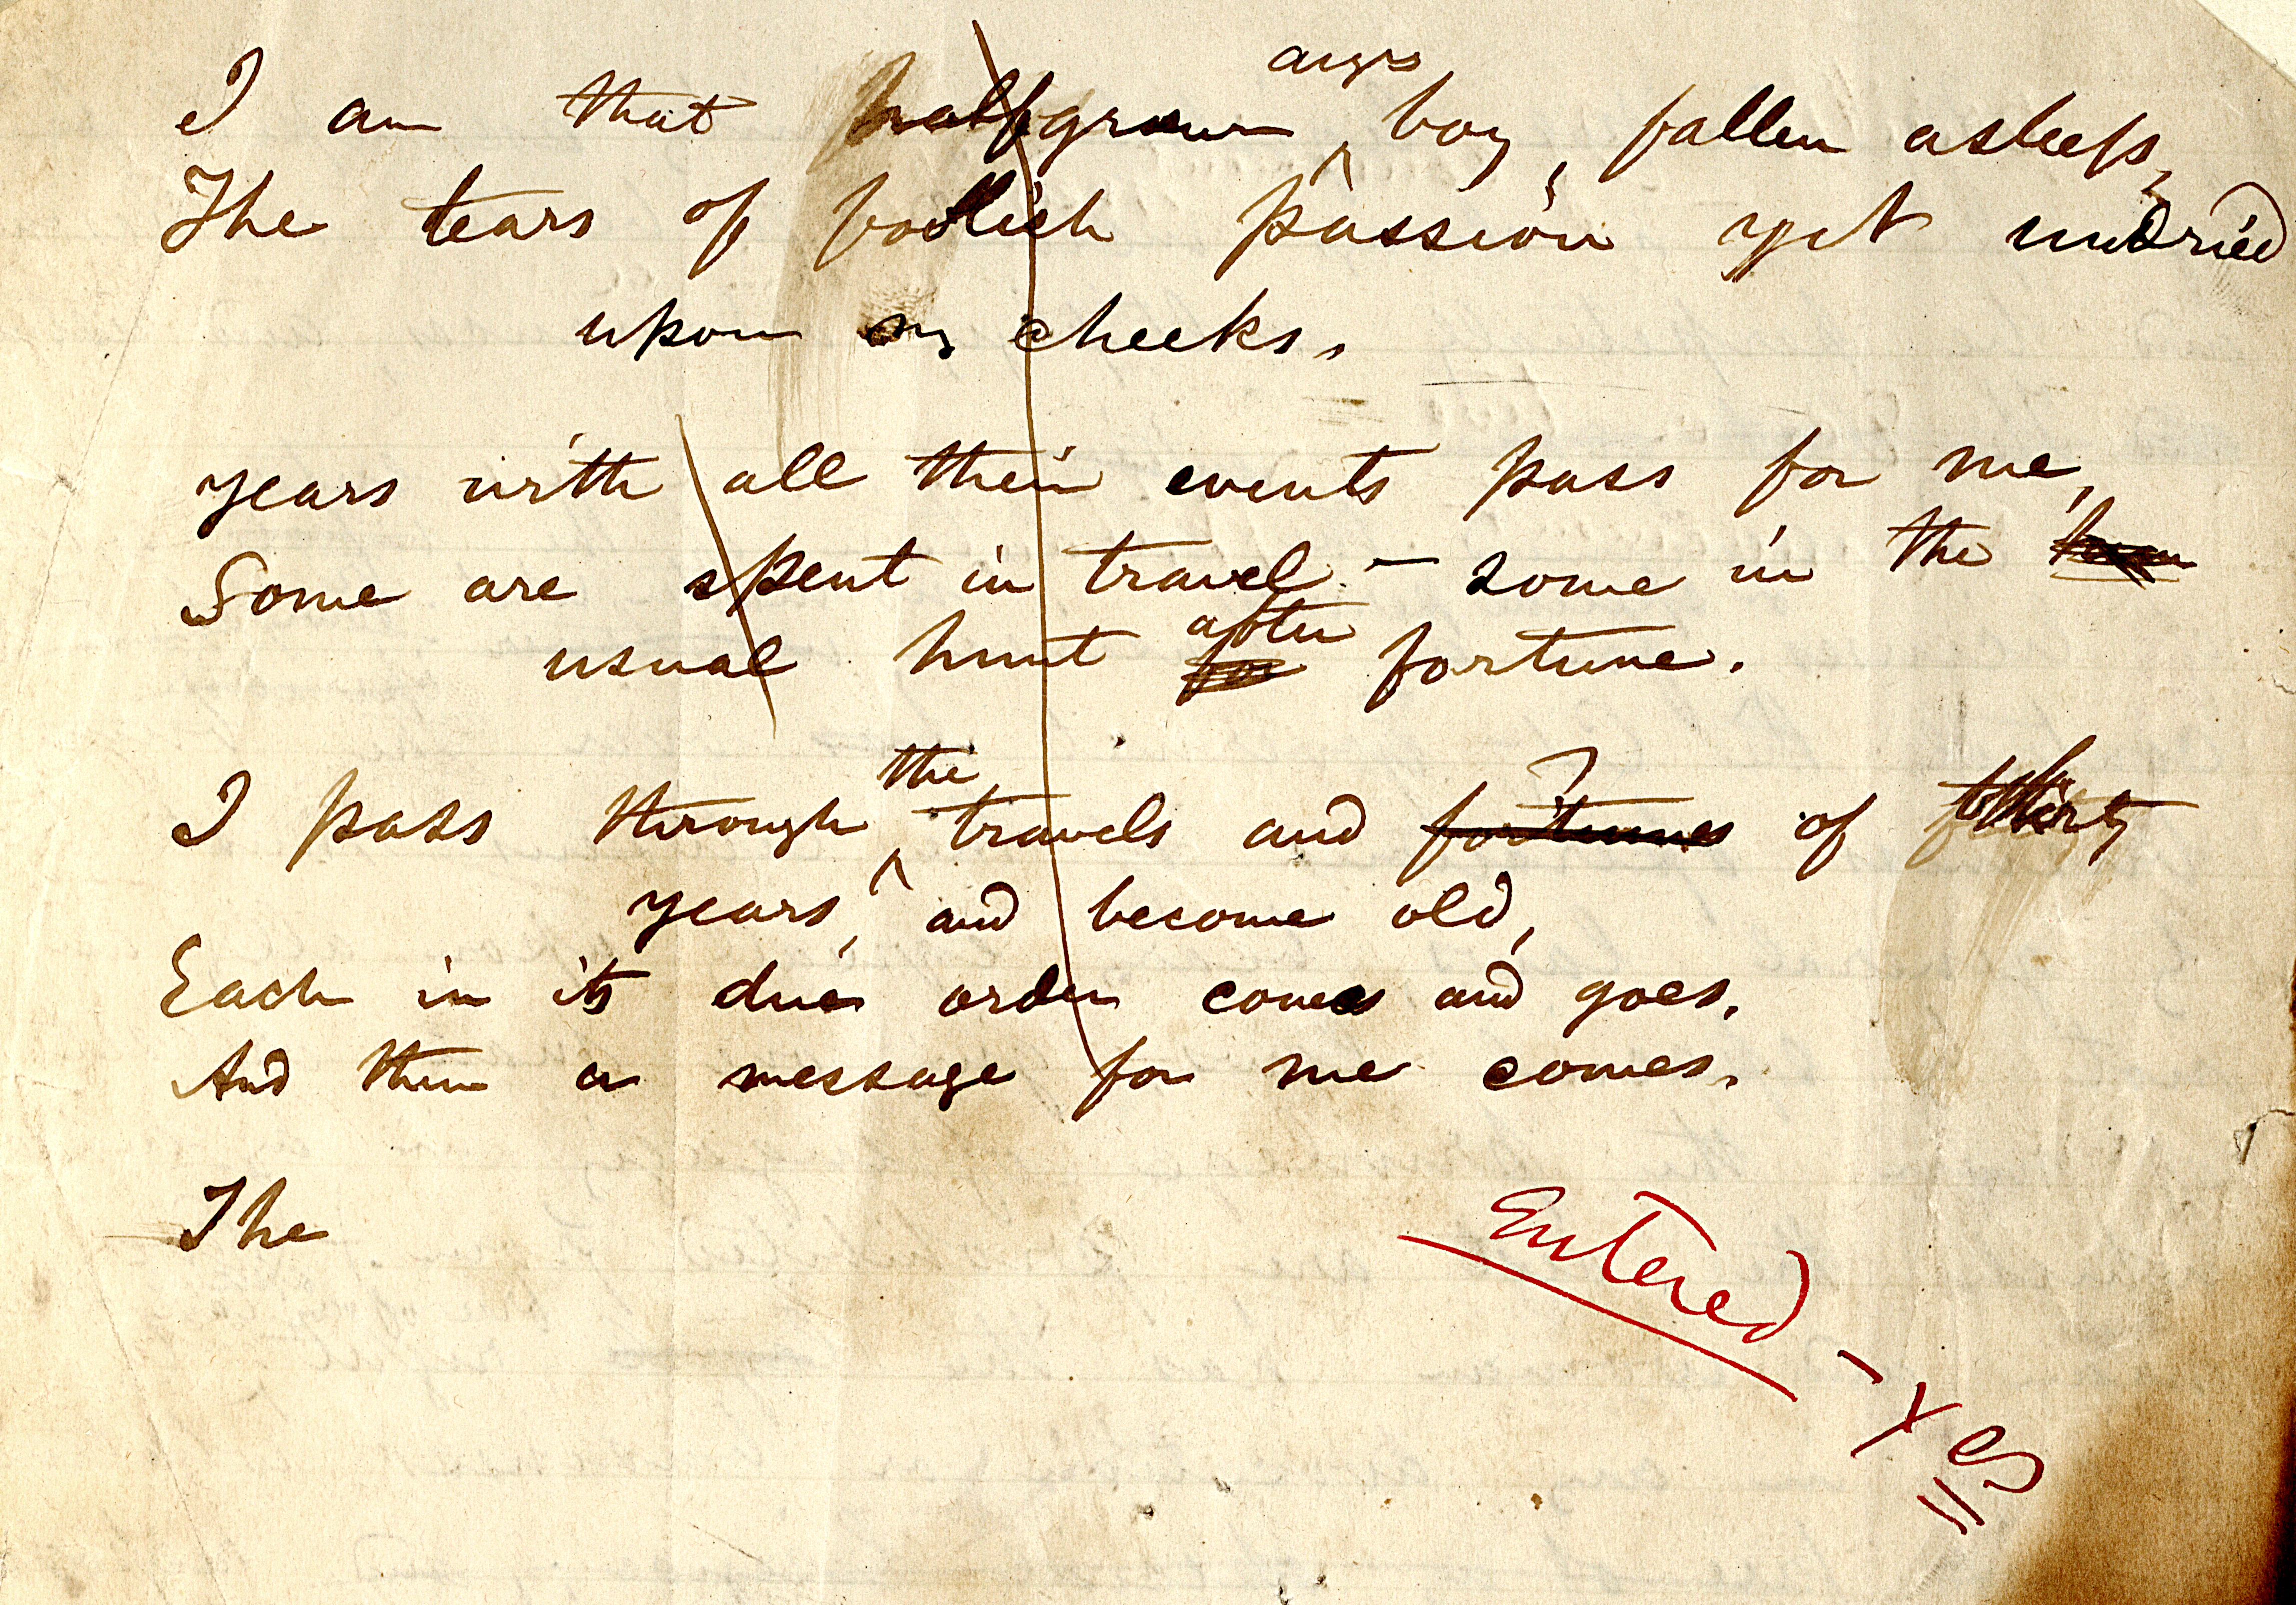
\includegraphics[width=0.7\textwidth,]{Images/whitman-02.jpg}
\caption{From "I am that halfgrown angry boy" (MS q 25), David M. Rubenstein Rare Book \& Manuscript Library, Duke University. }\end{figure}
\par
This page contains internal deletions, additions, and retracings but these are semantically quite different from the apparent ‘deletion’ signalled by the larger of the two single vertical lines, which shows that the written material has been transferred or re-used, not deleted.\par\bgroup\index{surface=<surface>|exampleindex}\index{metamark=<metamark>|exampleindex}\index{function=@function!<metamark>|exampleindex}\index{rend=@rend!<metamark>|exampleindex}\index{target=@target!<metamark>|exampleindex}\index{zone=<zone>|exampleindex}\index{line=<line>|exampleindex}\index{add=<add>|exampleindex}\index{line=<line>|exampleindex}\index{line=<line>|exampleindex}\index{line=<line>|exampleindex}\index{add=<add>|exampleindex}\index{del=<del>|exampleindex}\index{retrace=<retrace>|exampleindex}\index{line=<line>|exampleindex}\index{line=<line>|exampleindex}\index{line=<line>|exampleindex}\index{line=<line>|exampleindex}\index{metamark=<metamark>|exampleindex}\index{function=@function!<metamark>|exampleindex}\index{target=@target!<metamark>|exampleindex}\exampleFont \begin{shaded}\noindent\mbox{}{<\textbf{surface}>}\mbox{}\newline 
\hspace*{1em}{<\textbf{metamark}\hspace*{1em}{function}="{used}"\hspace*{1em}{rend}="{line}"\mbox{}\newline 
\hspace*{1em}\hspace*{1em}{target}="{\#X2}"/>}\mbox{}\newline 
\hspace*{1em}{<\textbf{zone}\hspace*{1em}{xml:id}="{X2}">}\mbox{}\newline 
\hspace*{1em}\hspace*{1em}{<\textbf{line}>}I am that halfgrown {<\textbf{add}>}angry{</\textbf{add}>} boy, fallen asleep{</\textbf{line}>}\mbox{}\newline 
\hspace*{1em}\hspace*{1em}{<\textbf{line}>}The tears of foolish passion yet undried{</\textbf{line}>}\mbox{}\newline 
\hspace*{1em}\hspace*{1em}{<\textbf{line}>}upon my cheeks.{</\textbf{line}>}\mbox{}\newline 
\textit{<!-- ... -->}\mbox{}\newline 
\hspace*{1em}\hspace*{1em}{<\textbf{line}>}I pass through {<\textbf{add}>}the{</\textbf{add}>} travels and {<\textbf{del}>}fortunes{</\textbf{del}>} of\mbox{}\newline 
\hspace*{1em}\hspace*{1em}{<\textbf{retrace}>}thirty{</\textbf{retrace}>}\mbox{}\newline 
\hspace*{1em}\hspace*{1em}{</\textbf{line}>}\mbox{}\newline 
\hspace*{1em}\hspace*{1em}{<\textbf{line}>}years and become old,{</\textbf{line}>}\mbox{}\newline 
\hspace*{1em}\hspace*{1em}{<\textbf{line}>}Each in its due order comes and goes,{</\textbf{line}>}\mbox{}\newline 
\hspace*{1em}\hspace*{1em}{<\textbf{line}>}And thus a message for me comes.{</\textbf{line}>}\mbox{}\newline 
\hspace*{1em}\hspace*{1em}{<\textbf{line}>}The{</\textbf{line}>}\mbox{}\newline 
\hspace*{1em}{</\textbf{zone}>}\mbox{}\newline 
\hspace*{1em}{<\textbf{metamark}\hspace*{1em}{function}="{used}"\hspace*{1em}{target}="{\#X2}">}Entered - Yes{</\textbf{metamark}>}\mbox{}\newline 
{</\textbf{surface}>}\end{shaded}\egroup\par \par
In this embedded transcription example, we class as metamarks both the long vertical line and the annotation ‘Entered - yes’.  Both metamarks are assumed to indicate that the whole of the written zone with identifier \texttt{X2} is marked as having been used. \hyperref[TEI.metamark]{<metamark>} can be similarly used within \hyperref[TEI.text]{<text>} to encode the same phenomenon as part of a transcription that privileges logical over physical and layout structures.
\paragraph[{Fixation and Clarification}]{Fixation and Clarification}\label{PH-fix}\par
A writer may sometimes rewrite material a second time without significant change and in the same place. We consider this a distinct activity from addition as usually defined because no new textual material results; instead the status of existing material is reaffirmed. We may distinguish two variants of this: \textit{fixation} where the first version was a tentative draft which is subsequently reaffirmed, for example by inking it over; and \textit{clarification}, where the first version was badly written and has been rewritten for clarity. The element \hyperref[TEI.retrace]{<retrace>} is provided for both cases; its {\itshape cause} attribute may be used to distinguish these or other cases. 
\begin{sansreflist}
  
\item [\textbf{<retrace>}] contains a sequence of writing which has been retraced, for example by over-inking, to clarify or fix it.
\end{sansreflist}
\par
In this simple example, taken from the papers of Henrik Ibsen, the writer wrote the word \textit{skuldren} hastily, and then returned to it to make the letter \textit{l} larger and clearer: \begin{figure}[htbp]
\noindent\noindent\includegraphics[width=400pt,]{Images/skuldren.jpg}
\caption{From autograph ms of \textit{Peer Gynt}, Collin 2869, 4°, I.1.1, the Royal Library of Copenhagen}\end{figure}
 We might transcribe this word as follows: \par\bgroup\index{retrace=<retrace>|exampleindex}\index{cause=@cause!<retrace>|exampleindex}\exampleFont \begin{shaded}\noindent\mbox{} Sku{<\textbf{retrace}\hspace*{1em}{cause}="{unclear}">}l{</\textbf{retrace}>}dren\mbox{}\newline 
\end{shaded}\egroup\par \par
A single rewrite may not be sufficient, and it may be that the document becomes almost unreadable as a result of repeated clarification. In the following example, we can distinguish at least three attempts to write the letters \textit{er} in the word \textit{bægerklang}: \begin{figure}[htbp]
\noindent\noindent\includegraphics[width=400pt,]{Images/munch01.jpg}
\caption{Detail from autograph ms \textit{Brand} in The Royal Library, Denmark (KBK Collin 262)}\end{figure}
 We might encode this by nesting the \hyperref[TEI.retrace]{<retrace>} element as follows: \par\bgroup\index{retrace=<retrace>|exampleindex}\index{cause=@cause!<retrace>|exampleindex}\index{change=@change!<retrace>|exampleindex}\index{retrace=<retrace>|exampleindex}\index{cause=@cause!<retrace>|exampleindex}\index{change=@change!<retrace>|exampleindex}\exampleFont \begin{shaded}\noindent\mbox{} ved Bæg{<\textbf{retrace}\hspace*{1em}{cause}="{unclear}"\hspace*{1em}{change}="{\#stage2}">}\mbox{}\newline 
\hspace*{1em}{<\textbf{retrace}\hspace*{1em}{cause}="{unclear}"\hspace*{1em}{change}="{\#stage1}">}er{</\textbf{retrace}>}\mbox{}\newline 
{</\textbf{retrace}>} ...\mbox{}\newline 
\end{shaded}\egroup\par \noindent  The {\itshape change} attribute used here is discussed further below (\textit{\hyperref[PH-changes]{11.7.\ Identifying Changes and Revisions}}).\par
The \hyperref[TEI.retrace]{<retrace>} element is used only for cases where text has been written multiple times. When metamarks and other markup-like strokes have been rewritten multiple times, the \hyperref[TEI.redo]{<redo>} element described in the next section should be used in preference.
\paragraph[{Confirmation, Cancellation, and Reinstatement of Modifications}]{Confirmation, Cancellation, and Reinstatement of Modifications}\label{undo}\par
 A writer may  indicate that an alteration is itself to be altered: for example, a struck-through passage may be restored via a dotted underlining, or the underlining of a passage may be deleted by a wavy line.\par
The following elements are provided to represent these situations: 
\begin{sansreflist}
  
\item [\textbf{<redo>}] indicates one or more cancelled interventions in a document which have subsequently been marked as reaffirmed or repeated.\hfil\\[-10pt]\begin{sansreflist}
    \item[@{\itshape target}]
  points to one or more elements representing the interventions which are being reasserted.
\end{sansreflist}  
\item [\textbf{<undo>}] indicates one or more marked-up interventions in a document which have subsequently been marked for cancellation.\hfil\\[-10pt]\begin{sansreflist}
    \item[@{\itshape target}]
  points to one or more elements representing the interventions which are to be reverted or undone.
\end{sansreflist}  
\end{sansreflist}
\par
The element \hyperref[TEI.restore]{<restore>} (\textit{\hyperref[PHCD]{11.3.1.6.\ Cancellation of Deletions and Other Markings}}) is provided for the comparatively simple case where a simple deletion is marked as having been subsequently cancelled. The \hyperref[TEI.undo]{<undo>} element discussed here is more widely applicable and may be used for any kind of cancellation. It points to the element or elements which are being cancelled. These components need not be contiguous, provided that the cancellation is clearly a single act; each distinct act of cancellation requires a distinct \hyperref[TEI.undo]{<undo>} element, however. Either of the attributes {\itshape target} or {\itshape spanTo} may be used to indicate the passages concerned.\par
Consider the following imaginary example: \begin{figure}[htbp]
\noindent\noindent\includegraphics[width=0.8\textwidth,]{Images/undoing1.jpg}
\caption{Imaginary example demonstrating restoring and undoing}\end{figure}
 We hypothesize that the text has gone through three states or changes, as follows: \begin{enumerate}
\item This is just some sample text, we need a real example. 
\item This is not a real example.
\item This is just some text, not a real example.
\end{enumerate}\par
This sequence of events might be encoded as follows: \par\bgroup\index{del=<del>|exampleindex}\index{change=@change!<del>|exampleindex}\index{rend=@rend!<del>|exampleindex}\index{undo=<undo>|mainexampleindex}\index{spanTo=@spanTo!<undo>|exampleindex}\index{rend=@rend!<undo>|exampleindex}\index{change=@change!<undo>|exampleindex}\index{anchor=<anchor>|exampleindex}\index{undo=<undo>|mainexampleindex}\index{spanTo=@spanTo!<undo>|exampleindex}\index{rend=@rend!<undo>|exampleindex}\index{change=@change!<undo>|exampleindex}\index{anchor=<anchor>|exampleindex}\index{add=<add>|exampleindex}\index{change=@change!<add>|exampleindex}\exampleFont \begin{shaded}\noindent\mbox{} This is {<\textbf{del}\hspace*{1em}{change}="{\#s2}"\hspace*{1em}{rend}="{overstrike}">}\mbox{}\newline 
\hspace*{1em}{<\textbf{undo}\hspace*{1em}{spanTo}="{\#Xa}"\hspace*{1em}{rend}="{dotted}"\mbox{}\newline 
\hspace*{1em}\hspace*{1em}{change}="{\#s3}"/>}just some {<\textbf{anchor}\hspace*{1em}{xml:id}="{Xa}"/>} sample {<\textbf{undo}\hspace*{1em}{spanTo}="{\#Xb}"\hspace*{1em}{rend}="{dotted}"\mbox{}\newline 
\hspace*{1em}\hspace*{1em}{change}="{\#s3}"/>}text, {<\textbf{anchor}\hspace*{1em}{xml:id}="{Xb}"/>} we need\mbox{}\newline 
{</\textbf{del}>}\mbox{}\newline 
{<\textbf{add}\hspace*{1em}{change}="{\#s2}">}not{</\textbf{add}>} a real example.\mbox{}\newline 
\end{shaded}\egroup\par \noindent  using two \hyperref[TEI.undo]{<undo>} elements, each with a {\itshape spanTo} attribute, to delimit the two parts of the deletion which were reverted at change s3. Note that in this case, since {\itshape target} is not supplied, it is the effect of the parent element (the \hyperref[TEI.del]{<del>}) which is assumed to be undone.\par
Alternatively, we might more economically use the generic \hyperref[TEI.seg]{<seg>} element to delimit the two sequences whose deletion is being reverted, and then use the {\itshape target} attribute on a single \hyperref[TEI.undo]{<undo>} element: \par\bgroup\index{del=<del>|exampleindex}\index{change=@change!<del>|exampleindex}\index{rend=@rend!<del>|exampleindex}\index{seg=<seg>|exampleindex}\index{seg=<seg>|exampleindex}\index{add=<add>|exampleindex}\index{change=@change!<add>|exampleindex}\index{undo=<undo>|mainexampleindex}\index{target=@target!<undo>|exampleindex}\index{rend=@rend!<undo>|exampleindex}\index{change=@change!<undo>|exampleindex}\exampleFont \begin{shaded}\noindent\mbox{} This is {<\textbf{del}\hspace*{1em}{change}="{\#s2}"\hspace*{1em}{rend}="{overstrike}">}\mbox{}\newline 
\hspace*{1em}{<\textbf{seg}\hspace*{1em}{xml:id}="{X-a}">}just some{</\textbf{seg}>} sample {<\textbf{seg}\hspace*{1em}{xml:id}="{X-b}">}text{</\textbf{seg}>}, we\mbox{}\newline 
 need\mbox{}\newline 
{</\textbf{del}>}\mbox{}\newline 
{<\textbf{add}\hspace*{1em}{change}="{\#s2}">}not{</\textbf{add}>} a real example.\mbox{}\newline 
\mbox{}\newline 
{<\textbf{undo}\hspace*{1em}{target}="{\#X-a \#X-b}"\hspace*{1em}{rend}="{dotted}"\mbox{}\newline 
\hspace*{1em}{change}="{\#s3}"/>}\end{shaded}\egroup\par \noindent  
\paragraph[{Transpositions}]{Transpositions}\label{transpo}\par
A \textit{transposition} occurs when metamarks are found in a document indicating that passages should be moved to a different position. Typically this may be done using arrows, asterisks or numbers, or other means. By definition the result of a transposition is not present in the document, and should not therefore be encoded, if the intention is to represent the actual appearance of the document. Instead, the following elements may be used to indicate the intended reordering: 
\begin{sansreflist}
  
\item [\textbf{<listTranspose>}] supplies a list of transpositions, each of which is indicated at some point in a document typically by means of metamarks.
\item [\textbf{<transpose>}] describes a single textual transposition as an ordered list of at least two pointers specifying the order in which the elements indicated should be re-combined.
\end{sansreflist}
\par
Consider for example, the following extract from an Ibsen manuscript \begin{figure}[htbp]
\noindent\noindent\includegraphics[width=400pt,]{Images/ibsen01.jpg}
\caption{Extract from autograph \textit{Digte} (Poems) NBO Ms. 4º 1110a}\end{figure}
 The underlined numbers 1 and 2 here indicate that, although the word \textit{bör} precedes the word \textit{hör} in the text, the order of the two words should be reversed. We may encode this as follows: \par\bgroup\index{seg=<seg>|exampleindex}\index{metamark=<metamark>|exampleindex}\index{rend=@rend!<metamark>|exampleindex}\index{function=@function!<metamark>|exampleindex}\index{target=@target!<metamark>|exampleindex}\index{place=@place!<metamark>|exampleindex}\index{seg=<seg>|exampleindex}\index{metamark=<metamark>|exampleindex}\index{rend=@rend!<metamark>|exampleindex}\index{function=@function!<metamark>|exampleindex}\index{target=@target!<metamark>|exampleindex}\index{place=@place!<metamark>|exampleindex}\index{listTranspose=<listTranspose>|exampleindex}\index{transpose=<transpose>|exampleindex}\index{ptr=<ptr>|exampleindex}\index{target=@target!<ptr>|exampleindex}\index{ptr=<ptr>|exampleindex}\index{target=@target!<ptr>|exampleindex}\exampleFont \begin{shaded}\noindent\mbox{}{<\textbf{seg}\hspace*{1em}{xml:id}="{ib01}">}bör{</\textbf{seg}>}\mbox{}\newline 
{<\textbf{metamark}\hspace*{1em}{rend}="{underline}"\mbox{}\newline 
\hspace*{1em}{function}="{transposition}"\hspace*{1em}{target}="{\#ib01}"\hspace*{1em}{place}="{above}">}2.{</\textbf{metamark}>} og \mbox{}\newline 
{<\textbf{seg}\hspace*{1em}{xml:id}="{ib02}">}hör{</\textbf{seg}>}\mbox{}\newline 
{<\textbf{metamark}\hspace*{1em}{rend}="{underline}"\mbox{}\newline 
\hspace*{1em}{function}="{transposition}"\hspace*{1em}{target}="{\#ib02}"\hspace*{1em}{place}="{above}">}1.{</\textbf{metamark}>}\mbox{}\newline 
\textit{<!-- either nearby or elsewhere, typically inside <profileDesc> or <standOff>: -->}\mbox{}\newline 
{<\textbf{listTranspose}>}\mbox{}\newline 
\hspace*{1em}{<\textbf{transpose}>}\mbox{}\newline 
\hspace*{1em}\hspace*{1em}{<\textbf{ptr}\hspace*{1em}{target}="{\#ib02}"/>}\mbox{}\newline 
\hspace*{1em}\hspace*{1em}{<\textbf{ptr}\hspace*{1em}{target}="{\#ib01}"/>}\mbox{}\newline 
\hspace*{1em}{</\textbf{transpose}>}\mbox{}\newline 
{</\textbf{listTranspose}>}\end{shaded}\egroup\par \par
Note the use of the generic \hyperref[TEI.seg]{<seg>} element to identify the sections of text being transposed. The following example uses an embedded transcription approach, which typically identifies lines of writing with the \hyperref[TEI.line]{<line>} element. This makes it trivial to refer to the transposed line, but when encoding transposition within \hyperref[TEI.text]{<text>} the encoder will need to find a way to identify the line with another element, such as \hyperref[TEI.seg]{<seg>}.\begin{figure}[htbp]
\noindent\noindent\includegraphics[width=600pt,]{Images/ibsen04.jpg}
\caption{Detail from autograph ms of \textit{Den episke Brand} (KBK Collin 2869)}\end{figure}
 \par\bgroup\index{line=<line>|exampleindex}\index{metamark=<metamark>|exampleindex}\index{function=@function!<metamark>|exampleindex}\index{place=@place!<metamark>|exampleindex}\index{line=<line>|exampleindex}\index{metamark=<metamark>|exampleindex}\index{function=@function!<metamark>|exampleindex}\index{place=@place!<metamark>|exampleindex}\index{listTranspose=<listTranspose>|exampleindex}\index{transpose=<transpose>|exampleindex}\index{ptr=<ptr>|exampleindex}\index{target=@target!<ptr>|exampleindex}\index{ptr=<ptr>|exampleindex}\index{target=@target!<ptr>|exampleindex}\exampleFont \begin{shaded}\noindent\mbox{}{<\textbf{line}\hspace*{1em}{xml:id}="{ib3}">}\mbox{}\newline 
\hspace*{1em}{<\textbf{metamark}\hspace*{1em}{function}="{transposition}"\mbox{}\newline 
\hspace*{1em}\hspace*{1em}{place}="{margin-left}">}2.){</\textbf{metamark}>} thi da er du med Himmelen i Pagt; — \mbox{}\newline 
{</\textbf{line}>}\mbox{}\newline 
{<\textbf{line}\hspace*{1em}{xml:id}="{ib4}">}\mbox{}\newline 
\hspace*{1em}{<\textbf{metamark}\hspace*{1em}{function}="{transposition}"\mbox{}\newline 
\hspace*{1em}\hspace*{1em}{place}="{margin-left}">}1.){</\textbf{metamark}>} da kan du\mbox{}\newline 
 Folkets Jøkelhjerter tine;\mbox{}\newline 
{</\textbf{line}>}\mbox{}\newline 
\textit{<!-- either nearby or elsewhere, typically inside <profileDesc> or <standOff>: -->}\mbox{}\newline 
{<\textbf{listTranspose}>}\mbox{}\newline 
\hspace*{1em}{<\textbf{transpose}>}\mbox{}\newline 
\hspace*{1em}\hspace*{1em}{<\textbf{ptr}\hspace*{1em}{target}="{\#ib4}"/>}\mbox{}\newline 
\hspace*{1em}\hspace*{1em}{<\textbf{ptr}\hspace*{1em}{target}="{\#ib3}"/>}\mbox{}\newline 
\hspace*{1em}{</\textbf{transpose}>}\mbox{}\newline 
{</\textbf{listTranspose}>}\end{shaded}\egroup\par \noindent  When transposition is made, the whole element indicated is understood to be moved, not just its contents. In the above example, the metamarks are thus understood to be moved along with the lines to which they apply.\par
One or more \hyperref[TEI.listTranspose]{<listTranspose>} elements may be supplied either embedded within the text, in the \hyperref[TEI.profileDesc]{<profileDesc>} of the header, or in a \hyperref[TEI.standOff]{<standOff>} depending on local preference. Each \hyperref[TEI.listTranspose]{<listTranspose>} can contain one or more \hyperref[TEI.transpose]{<transpose>} elements, each of which defines a single transposition.
\paragraph[{Alternative Readings}]{Alternative Readings}\label{alter}\par
\begin{figure}[htbp]
\noindent\noindent\includegraphics[width=400pt,]{Images/moore04.png}
\caption{Detail from autograph manuscript of the second version of \textit{Lalla Rookh}, Pierpont Morgan MA 310}\end{figure}
 In this example two alternative readings are provided, but no preference is indicated. While the author apparently first composed the line ‘Alone before his native river -’, at some later point, he entertained the possibility of using the word \textit{beside} instead of \textit{before}. The manuscript supplies no indication of which word Moore favours at this point, although in fact, in the first printed edition of \textit{Lalla Rookh} the word \textit{beside} was chosen.\par
The element \hyperref[TEI.alt]{<alt>} provided by the \textsf{linking} module gives a simple way of encoding the state of this manuscript, as follows: \par\bgroup\index{seg=<seg>|exampleindex}\index{add=<add>|exampleindex}\index{place=@place!<add>|exampleindex}\index{alt=<alt>|exampleindex}\index{target=@target!<alt>|exampleindex}\index{mode=@mode!<alt>|exampleindex}\index{weights=@weights!<alt>|exampleindex}\exampleFont \begin{shaded}\noindent\mbox{}Alone {<\textbf{seg}\hspace*{1em}{xml:id}="{alt1}">}before{</\textbf{seg}>}\mbox{}\newline 
{<\textbf{add}\hspace*{1em}{place}="{above}"\hspace*{1em}{xml:id}="{alt2}">}beside{</\textbf{add}>} his native river ­—\mbox{}\newline 
\mbox{}\newline 
{<\textbf{alt}\hspace*{1em}{target}="{\#alt1 \#alt2}"\hspace*{1em}{mode}="{excl}"\mbox{}\newline 
\hspace*{1em}{weights}="{0 1}"/>}\end{shaded}\egroup\par \par
The {\itshape mode} attribute here indicates that the two possible readings indicated by the {\itshape target} attribute are mutually exclusive. The {\itshape weights} attribute indicates the relative importance or preference to be attached to the two readings on a scale running from zero (most improbable) to one (most probable). In this case, we have a very strong preference for the second reading because this is the one that appears in the published version of the poem. The \hyperref[TEI.alt]{<alt>} element is further discussed in section \textit{\hyperref[SAAT]{16.8.\ Alternation}}.
\paragraph[{Instant Corrections}]{Instant Corrections}\label{instantcorr}\par
The use of elements such as \hyperref[TEI.del]{<del>} and \hyperref[TEI.add]{<add>} necessarily implies that the modifications they indicate were made at some time after the original writing. An exception to this is where a false start or ‘instant’ correction has been identified: the author starts to write, and then immediately corrects what has been written.\par
The {\itshape instant} attribute defined by this module may be used on any element which is a member of the \textsf{att.editLike} class to modify this default assumption. When the value of {\itshape instant} is set to true, the addition or deletion is considered to belong to the same change as its parent element, while \texttt{false} means some change later than that of its parent.\par
An example of false start or instant correction can be seen in the following line: \begin{figure}[htbp]
\noindent\noindent\includegraphics[width=0.7\textwidth,]{Images/whitman03a.jpg}
\caption{Detail fron \textit{[I am a curse]}, one of the drafts for Whitman's \textit{Song of Myself}}\end{figure}
 in which we can detect the following sequence of events: \begin{enumerate}
\item The letter T is written and then immediately deleted
\item The word The is written, deleted, and replaced by the word His
\item The added word His is then deleted
\item The initial letter i of the words \textit{iron necklace} is overwritten with a capital I
\end{enumerate} To indicate that the first of these acts must have taken place during the main act of writing, before the other deletion and additions, we might encode this revision campaign as follows: \par\bgroup\index{del=<del>|exampleindex}\index{instant=@instant!<del>|exampleindex}\index{mod=<mod>|exampleindex}\index{type=@type!<mod>|exampleindex}\index{del=<del>|exampleindex}\index{add=<add>|exampleindex}\index{place=@place!<add>|exampleindex}\index{del=<del>|exampleindex}\index{rend=@rend!<del>|exampleindex}\index{mod=<mod>|exampleindex}\index{type=@type!<mod>|exampleindex}\index{del=<del>|exampleindex}\index{rend=@rend!<del>|exampleindex}\index{add=<add>|exampleindex}\index{place=@place!<add>|exampleindex}\exampleFont \begin{shaded}\noindent\mbox{}{<\textbf{del}\hspace*{1em}{instant}="{true}">}T{</\textbf{del}>}\mbox{}\newline 
{<\textbf{mod}\hspace*{1em}{type}="{subst}">}\mbox{}\newline 
\hspace*{1em}{<\textbf{del}>}The{</\textbf{del}>}\mbox{}\newline 
\hspace*{1em}{<\textbf{add}\hspace*{1em}{place}="{above}">}\mbox{}\newline 
\hspace*{1em}\hspace*{1em}{<\textbf{del}\hspace*{1em}{rend}="{overstrike}">}His{</\textbf{del}>}\mbox{}\newline 
\hspace*{1em}{</\textbf{add}>}\mbox{}\newline 
{</\textbf{mod}>}\mbox{}\newline 
{<\textbf{mod}\hspace*{1em}{type}="{subst}">}\mbox{}\newline 
\hspace*{1em}{<\textbf{del}\hspace*{1em}{rend}="{overwritten}">}i{</\textbf{del}>}\mbox{}\newline 
\hspace*{1em}{<\textbf{add}\hspace*{1em}{place}="{superimposed}">}I{</\textbf{add}>}\mbox{}\newline 
{</\textbf{mod}>}ron necklace\mbox{}\newline 
\end{shaded}\egroup\par 
\subsection[{Aspects of Layout}]{Aspects of Layout}\label{PHLAY}\par
The following methods are available to capture general aspects of the layout of material on a page where this is considered important. Within the \hyperref[TEI.sourceDoc]{<sourceDoc>} element, as already indicated, the element \hyperref[TEI.surface]{<surface>} and \hyperref[TEI.surfaceGrp]{<surfaceGrp>} enable the encoder to represent directly the structure of a codex as gatherings or quires, leaves, and surfaces, as in the following example: \par\bgroup\index{sourceDoc=<sourceDoc>|exampleindex}\index{surfaceGrp=<surfaceGrp>|exampleindex}\index{type=@type!<surfaceGrp>|exampleindex}\index{n=@n!<surfaceGrp>|exampleindex}\index{surfaceGrp=<surfaceGrp>|exampleindex}\index{type=@type!<surfaceGrp>|exampleindex}\index{n=@n!<surfaceGrp>|exampleindex}\index{surface=<surface>|exampleindex}\index{type=@type!<surface>|exampleindex}\index{n=@n!<surface>|exampleindex}\index{surface=<surface>|exampleindex}\index{type=@type!<surface>|exampleindex}\index{n=@n!<surface>|exampleindex}\index{surfaceGrp=<surfaceGrp>|exampleindex}\index{type=@type!<surfaceGrp>|exampleindex}\index{n=@n!<surfaceGrp>|exampleindex}\index{surface=<surface>|exampleindex}\index{type=@type!<surface>|exampleindex}\index{n=@n!<surface>|exampleindex}\index{surface=<surface>|exampleindex}\index{type=@type!<surface>|exampleindex}\index{n=@n!<surface>|exampleindex}\exampleFont \begin{shaded}\noindent\mbox{}{<\textbf{sourceDoc}>}\mbox{}\newline 
\hspace*{1em}{<\textbf{surfaceGrp}\hspace*{1em}{type}="{quire}"\hspace*{1em}{n}="{1}">}\mbox{}\newline 
\hspace*{1em}\hspace*{1em}{<\textbf{surfaceGrp}\hspace*{1em}{type}="{leaf}"\hspace*{1em}{n}="{1}">}\mbox{}\newline 
\hspace*{1em}\hspace*{1em}\hspace*{1em}{<\textbf{surface}\hspace*{1em}{type}="{recto}"\hspace*{1em}{n}="{1r}">}\mbox{}\newline 
\textit{<!-- ... -->}\mbox{}\newline 
\hspace*{1em}\hspace*{1em}\hspace*{1em}{</\textbf{surface}>}\mbox{}\newline 
\hspace*{1em}\hspace*{1em}\hspace*{1em}{<\textbf{surface}\hspace*{1em}{type}="{verso}"\hspace*{1em}{n}="{1v}">}\mbox{}\newline 
\textit{<!-- ... -->}\mbox{}\newline 
\hspace*{1em}\hspace*{1em}\hspace*{1em}{</\textbf{surface}>}\mbox{}\newline 
\hspace*{1em}\hspace*{1em}{</\textbf{surfaceGrp}>}\mbox{}\newline 
\hspace*{1em}\hspace*{1em}{<\textbf{surfaceGrp}\hspace*{1em}{type}="{leaf}"\hspace*{1em}{n}="{2}">}\mbox{}\newline 
\hspace*{1em}\hspace*{1em}\hspace*{1em}{<\textbf{surface}\hspace*{1em}{type}="{recto}"\hspace*{1em}{n}="{2r}">}\mbox{}\newline 
\textit{<!-- ... -->}\mbox{}\newline 
\hspace*{1em}\hspace*{1em}\hspace*{1em}{</\textbf{surface}>}\mbox{}\newline 
\hspace*{1em}\hspace*{1em}\hspace*{1em}{<\textbf{surface}\hspace*{1em}{type}="{verso}"\hspace*{1em}{n}="{2v}">}\mbox{}\newline 
\textit{<!-- ... -->}\mbox{}\newline 
\hspace*{1em}\hspace*{1em}\hspace*{1em}{</\textbf{surface}>}\mbox{}\newline 
\hspace*{1em}\hspace*{1em}{</\textbf{surfaceGrp}>}\mbox{}\newline 
\textit{<!-- other leaves in first quire -->}\mbox{}\newline 
\hspace*{1em}{</\textbf{surfaceGrp}>}\mbox{}\newline 
\textit{<!-- other quires here -->}\mbox{}\newline 
{</\textbf{sourceDoc}>}\end{shaded}\egroup\par \par
In some cases, it may be preferable to define \hyperref[TEI.surface]{<surface>}s corresponding with each two page opening, for example where it is clear that the writer regarded each such opening as a single writing surface, with written zones or other features crossing the page divide. An example is shown here: \begin{figure}[htbp]
\noindent\noindent\includegraphics[width=0.8\textwidth,]{Images/proust-42v.png}
\caption{Opening from autograph ms of Proust's \textit{A la recherche du temps perdu} (f 42v-43r)}\end{figure}
\par
The coloured lines added to this image indicate a number of zones of writing, colour coded to indicate the order in which they were written (purple, then green, then red). For example, the zone marked in red on the left contains a note referring to the purple zone on the right. \par
This approach assumes that the transcription will primarily be organized in the same way as the physical layout of the source, using embedded transcription elements. Alternatively, where the a non-embedded transcription has been provided, using the \hyperref[TEI.text]{<text>} element, it is still possible to record gathering breaks, page breaks, column breaks, line breaks etc in the source, using the elements described in section \textit{\hyperref[CORS]{3.11.\ Reference Systems}}. Detailed metadata about the physical make-up of a source will usually be summarized by the \hyperref[TEI.physDesc]{<physDesc>} component of an \hyperref[TEI.msDesc]{<msDesc>} element discussed in \textit{\hyperref[msph]{10.7.\ Physical Description}}.
\subsubsection[{Space}]{Space}\label{PHSP}\par
The author or scribe may have left space for a word, or for an initial capital, and for some reason the word or capital was never supplied and the space left empty. The presence of significant space in the text being transcribed may be indicated by the \hyperref[TEI.space]{<space>} element. 
\begin{sansreflist}
  
\item [\textbf{<space>}] (space) indicates the location of a significant space in the text.\hfil\\[-10pt]\begin{sansreflist}
    \item[@{\itshape resp}]
  (responsible party) (responsible party) indicates the individual responsible for identifying and measuring the space
\end{sansreflist}  
\end{sansreflist}
 Note that this element should not be used to mark normal inter-word space or the like.\par
In line 694 of Chaucer's \textit{Wife of Bath's Prologue} in the Holkham manuscript the scribe has left a space for a word where other manuscripts read \textit{preestes}: \par\bgroup\index{space=<space>|exampleindex}\index{quantity=@quantity!<space>|exampleindex}\index{unit=@unit!<space>|exampleindex}\exampleFont \begin{shaded}\noindent\mbox{}By\mbox{}\newline 
 god if wommen had writen storyes As {<\textbf{space}\hspace*{1em}{quantity}="{7}"\hspace*{1em}{unit}="{chars}"/>} han within her\mbox{}\newline 
 oratoryes\end{shaded}\egroup\par \noindent  The \hyperref[TEI.supplied]{<supplied>} element discussed in the previous section may be used to supply the text presumed missing: \par\bgroup\index{supplied=<supplied>|exampleindex}\index{reason=@reason!<supplied>|exampleindex}\index{resp=@resp!<supplied>|exampleindex}\index{source=@source!<supplied>|exampleindex}\exampleFont \begin{shaded}\noindent\mbox{}By god if wommen had writen storyes As\mbox{}\newline 
{<\textbf{supplied}\hspace*{1em}{reason}="{space}"\hspace*{1em}{resp}="{\#ETD}"\mbox{}\newline 
\hspace*{1em}{source}="{\#Hg}">}preestes{</\textbf{supplied}>} han within\mbox{}\newline 
 her oratoryes\end{shaded}\egroup\par \noindent  Here, the fact of the space within the manuscript is indicated by the value of the {\itshape reason} attribute. The source of the supplied text is shown by the value of the {\itshape source} attribute as the Hengwrt manuscript; the transcriber responsible for supplying the text is ES.
\subsubsection[{Lines}]{Lines}\label{PHLN}\par
One of the more common forms of modification encountered in written documents of any kind is the presence of lines written under, beside, or through the text. Such lines may be of various types: they may be solid, dashed or dotted, doubled or tripled, wavy or straight, or a combination of these and other renderings. The line may be used for emphasis, or to mark a foreign or technical term, or to signal a quotation or a title, etc.: the elements \hyperref[TEI.emph]{<emph>}, \hyperref[TEI.foreign]{<foreign>}, \hyperref[TEI.term]{<term>}, \hyperref[TEI.mentioned]{<mentioned>}, or \hyperref[TEI.title]{<title>} may be used for these. Where the line has a clear paratextual function the \hyperref[TEI.metamark]{<metamark>} element may be considered more appropriate. Frequently, a scholar may judge that a line is used to delete text: the \hyperref[TEI.del]{<del>} element is available to indicate this. In all these cases, the {\itshape rend} attribute may be used to supply further details concerning the style of the line. Thus, Lawrence's deletion by strike-through of \textit{my} in the autograph of \textit{Eloi, Eloi, lama sabachthani} may be encoded: \par\bgroup\index{del=<del>|exampleindex}\index{rend=@rend!<del>|exampleindex}\index{hand=@hand!<del>|exampleindex}\exampleFont \begin{shaded}\noindent\mbox{}For I hate this {<\textbf{del}\hspace*{1em}{rend}="{strikethrough}"\hspace*{1em}{hand}="{\#dhl}">}my{</\textbf{del}>} body, which is so\mbox{}\newline 
 dear to me\end{shaded}\egroup\par \par
There will be instances, however, where a scholar wishes only to register the occurrence of lines in the text, without making any judgement as to what the lines signify. In these cases the \hyperref[TEI.hi]{<hi>} element may be used, with the {\itshape rend} attribute to mark the style of line. In the manuscript of a letter by Robert Browning to George Moulton-Barrett the underlining of the phrase \textit{had obtained all the letters to Mr Boyd} may be marked-up as follows: \par\bgroup\index{hi=<hi>|exampleindex}\index{rend=@rend!<hi>|exampleindex}\exampleFont \begin{shaded}\noindent\mbox{}I have once — by\mbox{}\newline 
 declaring I would prosecute by law — hindered a man's proceedings who {<\textbf{hi}\hspace*{1em}{rend}="{underline}">}had obtained all the letters to Mr Boyd{</\textbf{hi}>}\end{shaded}\egroup\par \par
The above examples presume the common case where a single word or phrase is marked by a line, with no doubt as to where the marking begins or ends and with no overlapping of the area of text with other marked areas of text. Where there is doubt, the \hyperref[TEI.certainty]{<certainty>} element may be used to record the doubt. In the Browning example cited above the underlining actually begins half-way under \textit{who}, and this uncertainty could be remarked as follows: \par\bgroup\index{hi=<hi>|exampleindex}\index{rend=@rend!<hi>|exampleindex}\index{certainty=<certainty>|exampleindex}\index{target=@target!<certainty>|exampleindex}\index{locus=@locus!<certainty>|exampleindex}\index{degree=@degree!<certainty>|exampleindex}\index{desc=<desc>|exampleindex}\exampleFont \begin{shaded}\noindent\mbox{}I have once — by declaring I would prosecute\mbox{}\newline 
 by law — hindered a man's proceedings who {<\textbf{hi}\hspace*{1em}{xml:id}="{cstart1}"\hspace*{1em}{rend}="{underline}">}had\mbox{}\newline 
 obtained all the letters to Mr Boyd{</\textbf{hi}>}\mbox{}\newline 
\textit{<!-- ... -->}\mbox{}\newline 
{<\textbf{certainty}\hspace*{1em}{target}="{\#cstart1}"\hspace*{1em}{locus}="{start}"\mbox{}\newline 
\hspace*{1em}{degree}="{0.70}">}\mbox{}\newline 
\hspace*{1em}{<\textbf{desc}>}may begin with previous word{</\textbf{desc}>}\mbox{}\newline 
{</\textbf{certainty}>}\end{shaded}\egroup\par \par
Where the area of text marked overlaps other areas of text, for example crossing a structural division, one of the spanning mechanisms mentioned above must be used; for example where the line is thought to mark a deletion, the \hyperref[TEI.delSpan]{<delSpan>} element may be used. Where it is desired simply to record the marking of a span of text in circumstances where it is not possible to surround the text with a \hyperref[TEI.hi]{<hi>} element, the \hyperref[TEI.span]{<span>} element may be used with the {\itshape rend} or {\itshape type} attribute indicating the style of line-marking.\par
More work needs to be done on clarifying the treatment of other textual features marked by lines which might so overlap or nest. For example, in many Middle English manuscripts (e.g. the Jesus and Digby verse collections), marginal sidebars may indicate metrical structure: couplets may be linked in pairs, with the pairs themselves linked into stanzas. Or, marginal sidebars may indicate emphasis, or may point out a region of text on which there is some annotation: in many manuscripts of Chaucer's \textit{Wife of Bath's Prologue} lines 655–8 are marked with nesting parentheses against which the scribe has written \textit{nota}.\par
Such features could be captured by use of the \hyperref[TEI.note]{<note>} element, containing a prose description of the manuscript at this point, enhanced by a link to a visual representation (or facsimile) of the feature in question. For example, in the Chaucer example just cited, one may wish to record that the \textit{nota} is written in the Hengwrt manuscript in the right margin against a single large left parenthesis bracketing the four lines, with two right parentheses in the right margin bracketing two overlapping pairs of lines: the first and third, the second and fourth. The \hyperref[TEI.note]{<note>} element allows us to record that the scribe wrote \textit{nota}, but is not well-adapted to show that the \textit{nota} points both at all four lines and at two pairs of lines within the four lines. The \hyperref[TEI.metamark]{<metamark>} element discussed in section \textit{\hyperref[PH-meta]{11.3.4.2.\ Metamarks}} above provides better facilities for this kind of complex annotation.
\subsection[{Transcription and Ruby}]{Transcription and Ruby}\label{PHRB}\par
These Guidelines also provide special elements to support the encoding of ruby annotations, which are common in East Asian textual traditions. These elements provide a method of capturing a specific type of annotation, in addition to the generic methods like the \hyperref[TEI.note]{<note>} or \hyperref[TEI.interp]{<interp>} elements. Both the specific and general methods should integrate well with the transcriptional elements described above, allowing authorial and scribal features to be captured in conjunction with ruby base text and annotations. See \textit{\hyperref[COHTGRB]{3.4.2.\ Ruby Annotations}} for more information about these elements.
\subsection[{Headers, Footers, and Similar Matter}]{Headers, Footers, and Similar Matter}\label{PHSK}\par
Such information as page numbers, signatures, or catchwords may be recorded in a specialized \hyperref[TEI.fw]{<fw>} element provided for that purpose. Although the name derives from the term \textit{forme work}, used in description of early printed documents (the ‘forme’ being the block used to hold movable type), the \hyperref[TEI.fw]{<fw>} element may be used for such features of any document, written or printed. Note that the purpose of this element is to record page numbers etc. \textit{actually present} in the document being encoded, not necessarily to provide a complete or accurate pagination of it.\par
Information about pagination etc. may also be provided using the {\itshape n} attribute of the \hyperref[TEI.pb]{<pb>} or \hyperref[TEI.gb]{<gb>} elements, or by other appropriate \hyperref[TEI.milestone]{<milestone>} elements, as further discussed in section \textit{\hyperref[CORS]{3.11.\ Reference Systems}}: since this information is usually provided by the encoder, it is not subject to the constraint that it should be present only if textually present in the source being encoded. In text-critical situations it may be useful to provide both a normalized version of the pagination and a representation of the catch-word or numbering, especially when the latter presents a variant reading, or is significant for compositor identification. 
\begin{sansreflist}
  
\item [\textbf{<fw>}] (forme work) contains a running head (e.g. a header, footer), catchword, or similar material appearing on the current page.
\end{sansreflist}
 The \hyperref[TEI.fw]{<fw>} element may be used to encode any of the unchanging portions of a page forme, such as: \begin{itemize}
\item running heads (whether repeated or changing on every page, or alternating pages)
\item running footers
\item page numbers
\item catch-words
\item other material repeated from page to page, which falls outside the stream of the text
\end{itemize}  It should not be used for marginal glosses, annotations, or textual variants, which should be tagged using \hyperref[TEI.gloss]{<gloss>}, \hyperref[TEI.note]{<note>}, or the text-critical tags described in chapter \textit{\hyperref[TC]{12.\ Critical Apparatus}}, respectively.\par
For example: \par\bgroup\index{fw=<fw>|exampleindex}\index{type=@type!<fw>|exampleindex}\index{place=@place!<fw>|exampleindex}\index{fw=<fw>|exampleindex}\index{type=@type!<fw>|exampleindex}\index{place=@place!<fw>|exampleindex}\index{fw=<fw>|exampleindex}\index{type=@type!<fw>|exampleindex}\index{place=@place!<fw>|exampleindex}\index{fw=<fw>|exampleindex}\index{type=@type!<fw>|exampleindex}\index{place=@place!<fw>|exampleindex}\exampleFont \begin{shaded}\noindent\mbox{}{<\textbf{fw}\hspace*{1em}{type}="{head}"\hspace*{1em}{place}="{top-centre}">}Poëms.{</\textbf{fw}>}\mbox{}\newline 
{<\textbf{fw}\hspace*{1em}{type}="{pageNum}"\hspace*{1em}{place}="{top-right}">}29{</\textbf{fw}>}\mbox{}\newline 
{<\textbf{fw}\hspace*{1em}{type}="{sig}"\hspace*{1em}{place}="{bot-centre}">}E3{</\textbf{fw}>}\mbox{}\newline 
{<\textbf{fw}\hspace*{1em}{type}="{catch}"\hspace*{1em}{place}="{bot-right}">}TEMPLE{</\textbf{fw}>}\end{shaded}\egroup\par \noindent    
\subsection[{Identifying Changes and Revisions}]{Identifying Changes and Revisions}\label{PH-changes}\par
A major purpose of genetic editing is the identification of ‘revision campaigns’ or, more generally, \textit{changes}. An editor may wish to regard a particular set of alterations (deletions, additions, substitutions, transpositions, etc.) or any other act of writing as a single object for which we use the general term \textit{change}, to indicate both that one or more of such phenomena preceded or followed another and also to indicate that they are related in some way, for example that one is a consequence of the other. They might also wish to group together certain revisions, regardless of when they might have occurred, based on a variety of other shared characteristics (e.g., corrections of factual errors or revisions that incorporate suggestions made by a given reader). To document this we need: \begin{itemize}
\item a system to assign phenomena to a particular ‘change’ as defined above
\item a way to characterize each such change, in itself and in relation to others.
\end{itemize} \par
The element \hyperref[TEI.creation]{<creation>} (within the TEI header profile description) contains all information relating to the genesis or production of a text. It may contain a \hyperref[TEI.listChange]{<listChange>} element which contains a number of \hyperref[TEI.change]{<change>} elements, one for each set of alterations identified: 
\begin{sansreflist}
  
\item [\textbf{<listChange>}] groups a number of change descriptions associated with either the creation of a source text or the revision of an encoded text.\hfil\\[-10pt]\begin{sansreflist}
    \item[@{\itshape ordered}]
  indicates whether the ordering of its child \hyperref[TEI.change]{<change>} elements is to be considered significant or not
\end{sansreflist}  
\item [\textbf{<change>}] (change) documents a change or set of changes made during the production of a source document, or during the revision of an electronic file.
\end{sansreflist}
\par
In the following example an editor has identified four distinct sets of alterations:\par\bgroup\index{profileDesc=<profileDesc>|exampleindex}\index{creation=<creation>|exampleindex}\index{listChange=<listChange>|exampleindex}\index{ordered=@ordered!<listChange>|exampleindex}\index{change=<change>|exampleindex}\index{change=<change>|exampleindex}\index{change=<change>|exampleindex}\index{change=<change>|exampleindex}\exampleFont \begin{shaded}\noindent\mbox{}{<\textbf{profileDesc}>}\mbox{}\newline 
\hspace*{1em}{<\textbf{creation}>}\mbox{}\newline 
\hspace*{1em}\hspace*{1em}{<\textbf{listChange}\hspace*{1em}{ordered}="{true}">}\mbox{}\newline 
\hspace*{1em}\hspace*{1em}\hspace*{1em}{<\textbf{change}\hspace*{1em}{xml:id}="{ST-1}">}First stage, written in ink {</\textbf{change}>}\mbox{}\newline 
\hspace*{1em}\hspace*{1em}\hspace*{1em}{<\textbf{change}\hspace*{1em}{xml:id}="{ST-2}">}Second stage, with revisions written in the author's hand\mbox{}\newline 
\hspace*{1em}\hspace*{1em}\hspace*{1em}\hspace*{1em}\hspace*{1em}\hspace*{1em} using pencil{</\textbf{change}>}\mbox{}\newline 
\hspace*{1em}\hspace*{1em}\hspace*{1em}{<\textbf{change}\hspace*{1em}{xml:id}="{ST-3}">}Fixation of the pencilled revisions together with further\mbox{}\newline 
\hspace*{1em}\hspace*{1em}\hspace*{1em}\hspace*{1em}\hspace*{1em}\hspace*{1em} revisions in the author's hand using ink{</\textbf{change}>}\mbox{}\newline 
\hspace*{1em}\hspace*{1em}\hspace*{1em}{<\textbf{change}\hspace*{1em}{xml:id}="{ST-4}">}Additions in a different hand, probably at a later\mbox{}\newline 
\hspace*{1em}\hspace*{1em}\hspace*{1em}\hspace*{1em}\hspace*{1em}\hspace*{1em} stage{</\textbf{change}>}\mbox{}\newline 
\hspace*{1em}\hspace*{1em}{</\textbf{listChange}>}\mbox{}\newline 
\hspace*{1em}{</\textbf{creation}>}\mbox{}\newline 
{</\textbf{profileDesc}>}\end{shaded}\egroup\par \par
The \hyperref[TEI.listChange]{<listChange>} element carries an attribute {\itshape ordered}, which can take the values \texttt{true} or \texttt{false} (the default). The attribute specifies whether the order of child elements signifies a temporal order for the revision campaigns which they document. In the example above, the editor has asserted that the four sets distinguished are ordered chronologically according to the order of the \hyperref[TEI.change]{<change>} elements.  If necessary, \hyperref[TEI.listChange]{<listChange>} elements can be nested hierarchically. This may be helpful in two cases. Firstly one can build up hypotheses about related revisions step-by-step, starting with \hyperref[TEI.change]{<change>} elements of smaller coverage, whose members are certainly related, and then in a subsequent pass grouping these in turn, thereby extending their reach.\par\bgroup\index{profileDesc=<profileDesc>|exampleindex}\index{creation=<creation>|exampleindex}\index{listChange=<listChange>|exampleindex}\index{change=<change>|exampleindex}\index{listChange=<listChange>|exampleindex}\index{change=<change>|exampleindex}\index{change=<change>|exampleindex}\index{change=<change>|exampleindex}\exampleFont \begin{shaded}\noindent\mbox{}{<\textbf{profileDesc}>}\mbox{}\newline 
\hspace*{1em}{<\textbf{creation}>}\mbox{}\newline 
\hspace*{1em}\hspace*{1em}{<\textbf{listChange}>}\mbox{}\newline 
\hspace*{1em}\hspace*{1em}\hspace*{1em}{<\textbf{change}\hspace*{1em}{xml:id}="{o}">}An unrelated change note{</\textbf{change}>}\mbox{}\newline 
\hspace*{1em}\hspace*{1em}\hspace*{1em}{<\textbf{listChange}\hspace*{1em}{xml:id}="{m}">}\mbox{}\newline 
\hspace*{1em}\hspace*{1em}\hspace*{1em}\hspace*{1em}{<\textbf{change}\hspace*{1em}{xml:id}="{m1}">}Alterations on one manuscript page, certainly\mbox{}\newline 
\hspace*{1em}\hspace*{1em}\hspace*{1em}\hspace*{1em}\hspace*{1em}\hspace*{1em}\hspace*{1em}\hspace*{1em} related{</\textbf{change}>}\mbox{}\newline 
\hspace*{1em}\hspace*{1em}\hspace*{1em}\hspace*{1em}{<\textbf{change}\hspace*{1em}{xml:id}="{m2}">}Alterations on another manuscript page, certainly\mbox{}\newline 
\hspace*{1em}\hspace*{1em}\hspace*{1em}\hspace*{1em}\hspace*{1em}\hspace*{1em}\hspace*{1em}\hspace*{1em} related{</\textbf{change}>}\mbox{}\newline 
\hspace*{1em}\hspace*{1em}\hspace*{1em}{</\textbf{listChange}>}\mbox{}\newline 
\hspace*{1em}\hspace*{1em}\hspace*{1em}{<\textbf{change}\hspace*{1em}{xml:id}="{p}">}Another unrelated change note{</\textbf{change}>}\mbox{}\newline 
\hspace*{1em}\hspace*{1em}{</\textbf{listChange}>}\mbox{}\newline 
\hspace*{1em}{</\textbf{creation}>}\mbox{}\newline 
{</\textbf{profileDesc}>}\end{shaded}\egroup\par \par
A nested \hyperref[TEI.listChange]{<listChange>} element is also useful to indicate a \textit{partial} ordering of \hyperref[TEI.change]{<change>} elements.\par\bgroup\index{listChange=<listChange>|exampleindex}\index{ordered=@ordered!<listChange>|exampleindex}\index{change=<change>|exampleindex}\index{listChange=<listChange>|exampleindex}\index{ordered=@ordered!<listChange>|exampleindex}\index{change=<change>|exampleindex}\index{change=<change>|exampleindex}\index{change=<change>|exampleindex}\exampleFont \begin{shaded}\noindent\mbox{}{<\textbf{listChange}\hspace*{1em}{ordered}="{true}">}\mbox{}\newline 
\hspace*{1em}{<\textbf{change}\hspace*{1em}{xml:id}="{ST1}">}The first stage{</\textbf{change}>}\mbox{}\newline 
\hspace*{1em}{<\textbf{listChange}\hspace*{1em}{ordered}="{false}">}\mbox{}\newline 
\textit{<!-- We have no information about the order of these changes, except\newline
     that they both followed ST1 and preceded STX  -->}\mbox{}\newline 
\hspace*{1em}\hspace*{1em}{<\textbf{change}\hspace*{1em}{xml:id}="{ST-rev1}">}A revision of the first stage{</\textbf{change}>}\mbox{}\newline 
\hspace*{1em}\hspace*{1em}{<\textbf{change}\hspace*{1em}{xml:id}="{ST-rev2}">}Another revision of the first stage{</\textbf{change}>}\mbox{}\newline 
\hspace*{1em}{</\textbf{listChange}>}\mbox{}\newline 
\hspace*{1em}{<\textbf{change}\hspace*{1em}{xml:id}="{STX}">}The last stage{</\textbf{change}>}\mbox{}\newline 
{</\textbf{listChange}>}\end{shaded}\egroup\par \par
In addition to the possibility of being ordered by their sequence within a \hyperref[TEI.listChange]{<listChange>} element, \hyperref[TEI.change]{<change>} elements may carry a number of attributes from the \textsf{att.datable} class ({\itshape period}, {\itshape when}, {\itshape notBefore}, {\itshape notAfter}, {\itshape from}, and {\itshape to}) which allow each element to be dated as exactly or inexactly as necessary, in the same way as is currently possible for the TEI \hyperref[TEI.date]{<date>} element.\par\bgroup\index{profileDesc=<profileDesc>|exampleindex}\index{creation=<creation>|exampleindex}\index{date=<date>|exampleindex}\index{notAfter=@notAfter!<date>|exampleindex}\index{listChange=<listChange>|exampleindex}\index{ordered=@ordered!<listChange>|exampleindex}\index{change=<change>|exampleindex}\index{when=@when!<change>|exampleindex}\index{title=<title>|exampleindex}\index{date=<date>|exampleindex}\index{q=<q>|exampleindex}\index{ref=<ref>|exampleindex}\index{target=@target!<ref>|exampleindex}\index{change=<change>|exampleindex}\index{notBefore=@notBefore!<change>|exampleindex}\index{date=<date>|exampleindex}\index{ref=<ref>|exampleindex}\index{target=@target!<ref>|exampleindex}\index{ref=<ref>|exampleindex}\index{target=@target!<ref>|exampleindex}\index{date=<date>|exampleindex}\index{ref=<ref>|exampleindex}\index{target=@target!<ref>|exampleindex}\index{date=<date>|exampleindex}\index{ref=<ref>|exampleindex}\index{target=@target!<ref>|exampleindex}\index{change=<change>|exampleindex}\index{notBefore=@notBefore!<change>|exampleindex}\index{date=<date>|exampleindex}\exampleFont \begin{shaded}\noindent\mbox{}{<\textbf{profileDesc}>}\mbox{}\newline 
\hspace*{1em}{<\textbf{creation}>}\mbox{}\newline 
\hspace*{1em}\hspace*{1em}{<\textbf{date}\hspace*{1em}{notAfter}="{1816-07-18}"/>}\mbox{}\newline 
\hspace*{1em}\hspace*{1em}{<\textbf{listChange}\hspace*{1em}{ordered}="{true}">}\mbox{}\newline 
\hspace*{1em}\hspace*{1em}\hspace*{1em}{<\textbf{change}\hspace*{1em}{xml:id}="{mod1}"\hspace*{1em}{when}="{1816-07-16}">}The first draft of\mbox{}\newline 
\hspace*{1em}\hspace*{1em}\hspace*{1em}{<\textbf{title}>}Persuasion{</\textbf{title}>}, completed by the date {<\textbf{date}>}July 16 1816{</\textbf{date}>}\mbox{}\newline 
\hspace*{1em}\hspace*{1em}\hspace*{1em}\hspace*{1em}\hspace*{1em}\hspace*{1em} which is written after the word {<\textbf{q}>}Finis{</\textbf{q}>} at {<\textbf{ref}\hspace*{1em}{target}="{\#pers-30}">}page\mbox{}\newline 
\hspace*{1em}\hspace*{1em}\hspace*{1em}\hspace*{1em}\hspace*{1em}\hspace*{1em}\hspace*{1em}\hspace*{1em} 30{</\textbf{ref}>}.{</\textbf{change}>}\mbox{}\newline 
\hspace*{1em}\hspace*{1em}\hspace*{1em}{<\textbf{change}\hspace*{1em}{xml:id}="{mod2}"\mbox{}\newline 
\hspace*{1em}\hspace*{1em}\hspace*{1em}\hspace*{1em}{notBefore}="{1816-07-16}">}After the {<\textbf{date}>}16th of July{</\textbf{date}>}\mbox{}\newline 
\hspace*{1em}\hspace*{1em}\hspace*{1em}\hspace*{1em}\hspace*{1em}\hspace*{1em} Austen starts revision of the two final chapters, by rewriting the end and\mbox{}\newline 
\hspace*{1em}\hspace*{1em}\hspace*{1em}\hspace*{1em}\hspace*{1em}\hspace*{1em} adding a new zone ({<\textbf{ref}\hspace*{1em}{target}="{\#transp-1}">}pages 32-35{</\textbf{ref}>}) to be inserted at\mbox{}\newline 
\hspace*{1em}\hspace*{1em}\hspace*{1em}{<\textbf{ref}\hspace*{1em}{target}="{\#insertion-p1}">}page 19{</\textbf{ref}>}. This stage is documented by the\mbox{}\newline 
\hspace*{1em}\hspace*{1em}\hspace*{1em}\hspace*{1em}\hspace*{1em}\hspace*{1em} deletion of the date ({<\textbf{date}>}July 16 1816{</\textbf{date}>}) at {<\textbf{ref}\hspace*{1em}{target}="{\#pers-30}">}page\mbox{}\newline 
\hspace*{1em}\hspace*{1em}\hspace*{1em}\hspace*{1em}\hspace*{1em}\hspace*{1em}\hspace*{1em}\hspace*{1em} 30{</\textbf{ref}>}, and the addition of more text and of a new date ({<\textbf{date}>}July 18.\mbox{}\newline 
\hspace*{1em}\hspace*{1em}\hspace*{1em}\hspace*{1em}\hspace*{1em}\hspace*{1em}\hspace*{1em}\hspace*{1em} 1816{</\textbf{date}>}) at {<\textbf{ref}\hspace*{1em}{target}="{\#pers-31}">}page 31{</\textbf{ref}>}\mbox{}\newline 
\hspace*{1em}\hspace*{1em}\hspace*{1em}{</\textbf{change}>}\mbox{}\newline 
\hspace*{1em}\hspace*{1em}\hspace*{1em}{<\textbf{change}\hspace*{1em}{notBefore}="{1816-07-18}">}Before publication, after {<\textbf{date}>}July 18th,\mbox{}\newline 
\hspace*{1em}\hspace*{1em}\hspace*{1em}\hspace*{1em}\hspace*{1em}\hspace*{1em}\hspace*{1em}\hspace*{1em} 1816{</\textbf{date}>} chapters 10-11 were broken into three chapters, 10, 11, 12, as\mbox{}\newline 
\hspace*{1em}\hspace*{1em}\hspace*{1em}\hspace*{1em}\hspace*{1em}\hspace*{1em} witnessed by the print.{</\textbf{change}>}\mbox{}\newline 
\hspace*{1em}\hspace*{1em}{</\textbf{listChange}>}\mbox{}\newline 
\hspace*{1em}{</\textbf{creation}>}\mbox{}\newline 
{</\textbf{profileDesc}>}\end{shaded}\egroup\par \par
Each \hyperref[TEI.change]{<change>} element, apart from declaring a distinct moment or phase in the creation of the document, may also contain references to other annotations contained within the \hyperref[TEI.teiHeader]{<teiHeader>} or in the document (as shown in the previous example). Such references, along with the textual content, are purely documentary. The association between a textual component and a \hyperref[TEI.change]{<change>} element is always made explicitly, either by using the {\itshape target} attribute on the \hyperref[TEI.change]{<change>} element to point to one or more textual elements, or by pointing from the element or elements concerned to the \hyperref[TEI.change]{<change>} element by means of their {\itshape change} attribute. If a \hyperref[TEI.change]{<change>} element is associated with some element, it is also associated with all of that element's children, unless otherwise indicated, for example by a new value for the {\itshape change} attribute.\par
In the following simple example, the text at one stage read ‘This is a mouse’, and at the next ‘This is a house mouse’: \par\bgroup\index{line=<line>|exampleindex}\index{change=@change!<line>|exampleindex}\index{add=<add>|exampleindex}\index{change=@change!<add>|exampleindex}\exampleFont \begin{shaded}\noindent\mbox{}{<\textbf{line}\hspace*{1em}{change}="{\#firstStage}">}This is a {<\textbf{add}\hspace*{1em}{change}="{\#secondStage}">}house{</\textbf{add}>}\mbox{}\newline 
 mouse.{</\textbf{line}>}\end{shaded}\egroup\par \par
In this example, however, the text originally read ‘This is a house’, and subsequently ‘This is a mouse’: \par\bgroup\index{line=<line>|exampleindex}\index{change=@change!<line>|exampleindex}\index{mod=<mod>|exampleindex}\index{type=@type!<mod>|exampleindex}\index{change=@change!<mod>|exampleindex}\index{del=<del>|exampleindex}\index{add=<add>|exampleindex}\exampleFont \begin{shaded}\noindent\mbox{}{<\textbf{line}\hspace*{1em}{change}="{\#firstStage}">}This is a {<\textbf{mod}\hspace*{1em}{type}="{subst}"\hspace*{1em}{change}="{\#secondStage}">}\mbox{}\newline 
\hspace*{1em}\hspace*{1em}{<\textbf{del}>}house{</\textbf{del}>}\mbox{}\newline 
\hspace*{1em}\hspace*{1em}{<\textbf{add}>}mouse{</\textbf{add}>}\mbox{}\newline 
\hspace*{1em}{</\textbf{mod}>}.{</\textbf{line}>}\end{shaded}\egroup\par \noindent  Note that in this case both the deletion and the addition are associated with the second \hyperref[TEI.change]{<change>} element. The word ‘house’, because its deletion forms part of this second set of alterations, must have been present originally, whereas the word ‘mouse’ must have been added during the second set of alterations.\par
Elements such as \hyperref[TEI.add]{<add>} and \hyperref[TEI.del]{<del>} and the like carry an implied semantics concerning the order in which events in the writing of a document was carried out: something which is deleted must have been written before it was deleted; something which is added must have been added at a later stage of the writing. Even when a combination of such elements is used, the chronology can usually be inferred (see further \textit{\hyperref[PHCOMB]{11.3.3.2.\ Use of the gap, del, damage, unclear, and supplied Elements in Combination}}). Explicit indication of the set of alterations to which some modification belongs is mostly useful in situations where all the alterations identified in a document are to be grouped, for example chronologically.\par
The interpretation of \hyperref[TEI.change]{<change>} elements with respect to a particular text passage is based on a number of implicit assumptions and constraints which have the effect of minimizing the amount of tagging necessary. The system is also flexible enough to support an explicit distinction between acts of writing and textual alterations, since either of these can be associated with changes described in the encoding. The following example shows an encoding in which the same passage is transcribed twice, once from a documentary perspective, and once from a textual one: \par\bgroup\index{profileDesc=<profileDesc>|exampleindex}\index{creation=<creation>|exampleindex}\index{listChange=<listChange>|exampleindex}\index{ordered=@ordered!<listChange>|exampleindex}\index{change=<change>|exampleindex}\index{target=@target!<change>|exampleindex}\index{change=<change>|exampleindex}\index{target=@target!<change>|exampleindex}\index{change=<change>|exampleindex}\index{target=@target!<change>|exampleindex}\index{sourceDoc=<sourceDoc>|exampleindex}\index{surface=<surface>|exampleindex}\index{zone=<zone>|exampleindex}\index{line=<line>|exampleindex}\index{handShift=<handShift>|exampleindex}\index{new=@new!<handShift>|exampleindex}\index{retrace=<retrace>|exampleindex}\index{hand=@hand!<retrace>|exampleindex}\index{line=<line>|exampleindex}\index{handShift=<handShift>|exampleindex}\index{new=@new!<handShift>|exampleindex}\index{line=<line>|exampleindex}\index{handShift=<handShift>|exampleindex}\index{new=@new!<handShift>|exampleindex}\index{retrace=<retrace>|exampleindex}\index{hand=@hand!<retrace>|exampleindex}\index{line=<line>|exampleindex}\index{text=<text>|exampleindex}\index{body=<body>|exampleindex}\index{l=<l>|exampleindex}\index{n=@n!<l>|exampleindex}\index{subst=<subst>|exampleindex}\index{del=<del>|exampleindex}\index{add=<add>|exampleindex}\index{l=<l>|exampleindex}\index{n=@n!<l>|exampleindex}\index{subst=<subst>|exampleindex}\index{del=<del>|exampleindex}\index{add=<add>|exampleindex}\exampleFont \begin{shaded}\noindent\mbox{}{<\textbf{profileDesc}>}\mbox{}\newline 
\hspace*{1em}{<\textbf{creation}>}\mbox{}\newline 
\hspace*{1em}\hspace*{1em}{<\textbf{listChange}\hspace*{1em}{ordered}="{true}">}\mbox{}\newline 
\hspace*{1em}\hspace*{1em}\hspace*{1em}{<\textbf{change}\hspace*{1em}{target}="{\#zone\textunderscore 1 \#subst\textunderscore 3}">}First stage, written in ink by a\mbox{}\newline 
\hspace*{1em}\hspace*{1em}\hspace*{1em}\hspace*{1em}\hspace*{1em}\hspace*{1em} scribe{</\textbf{change}>}\mbox{}\newline 
\hspace*{1em}\hspace*{1em}\hspace*{1em}{<\textbf{change}\hspace*{1em}{target}="{\#zone\textunderscore 2 \#mod\textunderscore 1 \#line\textunderscore 1 \#line\textunderscore 2 \#subst\textunderscore 1 \#subst\textunderscore 2 \#subst\textunderscore 4 \#delSpan\textunderscore 1}">}Revised by Goethe using pencil{</\textbf{change}>}\mbox{}\newline 
\hspace*{1em}\hspace*{1em}\hspace*{1em}{<\textbf{change}\hspace*{1em}{target}="{\#redo\textunderscore 1 \#redo\textunderscore 2 \#redo\textunderscore 3 \#subst\textunderscore 1 \#subst\textunderscore 2 \#delSpan\textunderscore 1 \#add\textunderscore 1}">}Fixation of the revised passages and further revisions by Goethe using\mbox{}\newline 
\hspace*{1em}\hspace*{1em}\hspace*{1em}\hspace*{1em}\hspace*{1em}\hspace*{1em} ink{</\textbf{change}>}\mbox{}\newline 
\hspace*{1em}\hspace*{1em}{</\textbf{listChange}>}\mbox{}\newline 
\hspace*{1em}{</\textbf{creation}>}\mbox{}\newline 
{</\textbf{profileDesc}>}\mbox{}\newline 
{<\textbf{sourceDoc}>}\mbox{}\newline 
\hspace*{1em}{<\textbf{surface}>}\mbox{}\newline 
\hspace*{1em}\hspace*{1em}{<\textbf{zone}\hspace*{1em}{xml:id}="{zone\textunderscore 1}">}\mbox{}\newline 
\hspace*{1em}\hspace*{1em}\hspace*{1em}{<\textbf{line}\hspace*{1em}{xml:id}="{line\textunderscore 1}">}\mbox{}\newline 
\hspace*{1em}\hspace*{1em}\hspace*{1em}\hspace*{1em}{<\textbf{handShift}\hspace*{1em}{new}="{\#g\textunderscore bl}"/>}\mbox{}\newline 
\hspace*{1em}\hspace*{1em}\hspace*{1em}\hspace*{1em}{<\textbf{retrace}\hspace*{1em}{hand}="{\#g\textunderscore t}"\hspace*{1em}{xml:id}="{redo\textunderscore 1}">}Nun{</\textbf{retrace}>}\mbox{}\newline 
\hspace*{1em}\hspace*{1em}\hspace*{1em}{</\textbf{line}>}\mbox{}\newline 
\hspace*{1em}\hspace*{1em}\hspace*{1em}{<\textbf{line}>}\mbox{}\newline 
\hspace*{1em}\hspace*{1em}\hspace*{1em}\hspace*{1em}{<\textbf{handShift}\hspace*{1em}{new}="{\#jo\textunderscore t}"/>}Ihr wanſtige Schuften mit den Feuerbacken{</\textbf{line}>}\mbox{}\newline 
\hspace*{1em}\hspace*{1em}\hspace*{1em}{<\textbf{line}\hspace*{1em}{xml:id}="{line\textunderscore 2}">}\mbox{}\newline 
\hspace*{1em}\hspace*{1em}\hspace*{1em}\hspace*{1em}{<\textbf{handShift}\hspace*{1em}{new}="{\#g\textunderscore bl}"/>}\mbox{}\newline 
\hspace*{1em}\hspace*{1em}\hspace*{1em}\hspace*{1em}{<\textbf{retrace}\hspace*{1em}{hand}="{\#g\textunderscore t}"\hspace*{1em}{xml:id}="{redo\textunderscore 2}">}feiſt{</\textbf{retrace}>}\mbox{}\newline 
\hspace*{1em}\hspace*{1em}\hspace*{1em}{</\textbf{line}>}\mbox{}\newline 
\hspace*{1em}\hspace*{1em}\hspace*{1em}{<\textbf{line}>}Ihr glüht ſo recht vom Höllen Schwefel ſatt.{</\textbf{line}>} [...] {</\textbf{zone}>}\mbox{}\newline 
\hspace*{1em}{</\textbf{surface}>}\mbox{}\newline 
{</\textbf{sourceDoc}>}\mbox{}\newline 
{<\textbf{text}>}\mbox{}\newline 
\hspace*{1em}{<\textbf{body}>}\mbox{}\newline 
\hspace*{1em}\hspace*{1em}{<\textbf{l}\hspace*{1em}{n}="{11656}">}\mbox{}\newline 
\hspace*{1em}\hspace*{1em}\hspace*{1em}{<\textbf{subst}\hspace*{1em}{xml:id}="{subst\textunderscore 1}">}\mbox{}\newline 
\hspace*{1em}\hspace*{1em}\hspace*{1em}\hspace*{1em}{<\textbf{del}>}Ihr{</\textbf{del}>}\mbox{}\newline 
\hspace*{1em}\hspace*{1em}\hspace*{1em}\hspace*{1em}{<\textbf{add}>}Nun{</\textbf{add}>}\mbox{}\newline 
\hspace*{1em}\hspace*{1em}\hspace*{1em}{</\textbf{subst}>} wanſtige Schuften mit den Feuerbacken{</\textbf{l}>}\mbox{}\newline 
\hspace*{1em}\hspace*{1em}{<\textbf{l}\hspace*{1em}{n}="{11657}">}Ihr glüht ſo recht vom Höllen Schwefel {<\textbf{subst}\hspace*{1em}{xml:id}="{subst\textunderscore 2}">}\mbox{}\newline 
\hspace*{1em}\hspace*{1em}\hspace*{1em}\hspace*{1em}{<\textbf{del}>}ſatt{</\textbf{del}>}\mbox{}\newline 
\hspace*{1em}\hspace*{1em}\hspace*{1em}\hspace*{1em}{<\textbf{add}>}feiſt{</\textbf{add}>}\mbox{}\newline 
\hspace*{1em}\hspace*{1em}\hspace*{1em}{</\textbf{subst}>}.{</\textbf{l}>}\mbox{}\newline 
\hspace*{1em}{</\textbf{body}>}\mbox{}\newline 
{</\textbf{text}>}\end{shaded}\egroup\par \par
The documentary transcription stresses the writing process, while the textual transcription emphasizes textual alterations. In either case, the change of writing activity associated with a particular feature in the transcript is explicitly indicated. From the documentary perspective, by assigning particular modifications to a specific \hyperref[TEI.change]{<change>} element, we describe the writing process, in that they specify which segment has been written when . From the textual perspective, the markup concentrates simply on the existence of textual alterations and makes no explicit claims about the order of writing. 
\subsection[{Other Primary Source Features not Covered in these Guidelines}]{Other Primary Source Features not Covered in these Guidelines}\label{PHTRXX}\par
We repeat the advice given at the beginning of this chapter, that these recommendations are not intended to meet every transcriptional circumstance ever likely to be faced by any scholar. They are intended rather as a base to enable encoding of the most common phenomena found in the course of scholarly transcription of primary source materials. These guidelines particularly do not address the encoding of physical description of textual witnesses: the materials of the carrier, the medium of the inscribing implement, the organisation of the carrier materials themselves (as quiring, collation, etc.), and authorial instructions or scribal markup, except insofar as these are involved in the broader question of manuscript description, as addressed by the \textsf{msdescription} module described in chapter \textit{\hyperref[MS]{10.\ Manuscript Description}}.
\subsection[{Module for Transcription of Primary Sources}]{Module for Transcription of Primary Sources}\par
The module described in this chapter makes available the following components: \begin{description}

\item[{Module transcr: Transcription of primary sources}]\hspace{1em}\hfill\linebreak
\mbox{}\\[-10pt] \begin{itemize}
\item {\itshape Elements defined}: \hyperref[TEI.addSpan]{addSpan} \hyperref[TEI.am]{am} \hyperref[TEI.damage]{damage} \hyperref[TEI.damageSpan]{damageSpan} \hyperref[TEI.delSpan]{delSpan} \hyperref[TEI.ex]{ex} \hyperref[TEI.facsimile]{facsimile} \hyperref[TEI.fw]{fw} \hyperref[TEI.handNotes]{handNotes} \hyperref[TEI.handShift]{handShift} \hyperref[TEI.line]{line} \hyperref[TEI.listTranspose]{listTranspose} \hyperref[TEI.metamark]{metamark} \hyperref[TEI.mod]{mod} \hyperref[TEI.path]{path} \hyperref[TEI.redo]{redo} \hyperref[TEI.restore]{restore} \hyperref[TEI.retrace]{retrace} \hyperref[TEI.secl]{secl} \hyperref[TEI.sourceDoc]{sourceDoc} \hyperref[TEI.space]{space} \hyperref[TEI.subst]{subst} \hyperref[TEI.substJoin]{substJoin} \hyperref[TEI.supplied]{supplied} \hyperref[TEI.surface]{surface} \hyperref[TEI.surfaceGrp]{surfaceGrp} \hyperref[TEI.surplus]{surplus} \hyperref[TEI.transpose]{transpose} \hyperref[TEI.undo]{undo} \hyperref[TEI.zone]{zone}
\item {\itshape Classes defined}: \hyperref[TEI.att.coordinated]{att.coordinated} \hyperref[TEI.att.global.change]{att.global.change} \hyperref[TEI.att.global.facs]{att.global.facs}
\end{itemize} 
\end{description}   The selection and combination of modules to form a TEI schema is described in \textit{\hyperref[STIN]{1.2.\ Defining a TEI Schema}}.